\newcommand{\DoNotLoadEpstopdf}{}
\documentclass[11pt]{article}
\pdftrailerid{}
\usepackage[T1]{fontenc}
\usepackage{lmodern}
\usepackage[margin=1.08in]{geometry}
\usepackage{amsmath,amssymb,amsthm,mathtools,mathrsfs}
\usepackage{microtype,enumitem}
\usepackage{tikz}
\usetikzlibrary{arrows.meta,positioning}
\usepackage[hidelinks]{hyperref}
\usepackage[capitalise,noabbrev]{cleveref}
\numberwithin{equation}{section}
\newtheorem{theorem}{Theorem}[section]
\newtheorem{proposition}[theorem]{Proposition}
\newtheorem{lemma}[theorem]{Lemma}
\newtheorem{corollary}[theorem]{Corollary}
\theoremstyle{definition}
\newtheorem{definition}[theorem]{Definition}
\theoremstyle{remark}
\newtheorem{remark}[theorem]{Remark}
\AddToHook{env/theorem/begin}{\crefalias{theorem}{theorem}}
\AddToHook{env/proposition/begin}{\crefalias{theorem}{proposition}}
\AddToHook{env/lemma/begin}{\crefalias{theorem}{lemma}}
\AddToHook{env/corollary/begin}{\crefalias{theorem}{corollary}}
\AddToHook{env/definition/begin}{\crefalias{theorem}{definition}}
\AddToHook{env/remark/begin}{\crefalias{theorem}{remark}}
\newcommand{\N}{\mathbb N}
\newcommand{\Z}{\mathbb Z}
\newcommand{\R}{\mathbb R}
\newcommand{\C}{\mathbb C}
\newcommand{\T}{\mathbb R/\mathbb Z}
\newcommand{\E}{\mathbb E}
\newcommand{\Pbb}{\mathbb P}
\newcommand{\1}{\mathbf 1}
\newcommand{\eps}{\varepsilon}
\DeclareMathOperator{\RePart}{Re}
\setlist{itemsep=3pt,topsep=5pt}
\setlength{\emergencystretch}{1.5em}
\title{Ordinary two-point correlations of multiplicative functions}
\author{OpenAI}
\hypersetup{
  pdftitle={Ordinary two-point correlations of multiplicative functions},
  pdfauthor={OpenAI}
}
\date{September 24, 2026}
\begin{document}
\maketitle
\begin{abstract}
We prove the ordinary two-point Chowla conjecture. For every fixed pair
of nonproportional affine forms, the Liouville correlation has a
power-of-logarithm saving at every cutoff, with an absolute exponent.
We also prove the binary corrected Elliott conjecture for ordinary
averages of complex multiplicative functions of modulus at most one,
under uniform nonpretentiousness of at least one original factor.
This qualitative conclusion holds in fixed residue classes and for
fixed nonproportional affine forms.
\end{abstract}
\tableofcontents
\section{Introduction}\label{sec:introduction}

For \(n\ge1\), let \(\Omega(n)\) be the number of prime factors of \(n\),
counted with multiplicity, and let \(\lambda(n)=(-1)^{\Omega(n)}\).
We study ordinary two-point averages: each integer up to the given
cutoff has weight one. Thus the correlation measures whether the two prime-factor counts
have the same parity more often than different parities on the full
initial interval.
The distinction from a logarithmic average is the distinction between
\[
 \frac1X\sum_{n\le X}a(n)
 \qquad\text{and}\qquad
 \frac1{\log X}\sum_{n\le X}\frac{a(n)}n.
\]
Logarithmic weighting combines information from many multiplicative
scales; an ordinary estimate must control the terminal scale itself.
Our quantitative conclusion concerns every fixed pair of
nonproportional affine forms.

\begin{theorem}[A logarithmic saving for affine Liouville correlations]
\label{thm:q-affine}
There is an absolute constant \(c>0\) such that, for every fixed choice
of integers \(a_1,a_2\ge1\) and \(b_1,b_2\ge0\) with
\(a_1b_2-a_2b_1\ne0\), there is a constant
\(C_{a_1,a_2,b_1,b_2}\) for which
\[
 \left|\sum_{1\le n\le X}
       \lambda(a_1n+b_1)\lambda(a_2n+b_2)\right|
 \le C_{a_1,a_2,b_1,b_2}\frac{X}{(\log X)^c}
 \qquad(X\ge3).
\]
The cutoff \(X\) may be any real number. No coprimality condition is
imposed on the coefficients.
\end{theorem}

For $a_1=a_2=1$ and $b_1=0$, $b_2=h>0$, this resolves the
ordinary two-point Chowla conjecture, with a logarithmic saving.
The exponent is independent of the forms. The implied constants need
not be effective, and no uniformity for coefficients growing with \(X\)
is asserted. The proof first obtains the same saving for
\(\lambda(n)\lambda(n+h)\) in each fixed residue class modulo each fixed
positive integer, including nonunit and zero classes. Complete
multiplicativity then gives the affine conclusion.

We also prove a qualitative statement for general multiplicative
functions. Let \(\mathbb D=\{z\in\C:|z|\le1\}\). A function
\(f:\N\to\mathbb D\) is multiplicative when
\(f(mn)=f(m)f(n)\) for coprime positive integers \(m,n\).
For a Dirichlet character \(\chi\), a real number \(t\), and \(X\ge2\),
define the nonnegative distance \(D\) by
\begin{equation}\label{eq:distance}
 D(f,\chi n^{it};X)^2
 =\sum_{p\le X}\frac{1-\operatorname{Re}
       (f(p)\overline{\chi(p)p^{it}})}p.
\end{equation}
All sums indexed by \(p\) are over primes. We call \(f\)
\emph{uniformly nonpretentious} if, for every fixed Dirichlet character,
\begin{equation}\label{eq:unp}
 \inf_{|t|\le N}D(f,\chi n^{it};N)\longrightarrow\infty
 \qquad(N\longrightarrow\infty).
\end{equation}
The prime cutoff and the height bound are the same \(N\).

\begin{theorem}[Binary corrected Elliott]\label{thm:elliott}
Let \(f_1,f_2:\N\to\mathbb D\) be multiplicative, and suppose that
at least one satisfies \eqref{eq:unp}. For every fixed pair of distinct
nonnegative integers \(h_1,h_2\),
\[
 \frac1N\sum_{n=1}^N f_1(n+h_1)f_2(n+h_2)\longrightarrow0
 \qquad(N\longrightarrow\infty,\ N\in\N).
\]
\end{theorem}

This proves the binary corrected Elliott conjecture for ordinary
averages. The functions may be complex, need not have modulus one,
and need not be completely multiplicative. There is no conjugation
in the displayed product; the conjugated version follows because
\eqref{eq:unp} is preserved by conjugation. We make no quantitative
rate claim for this class of functions.

\begin{corollary}[Affine correlations]\label{cor:affine}
Let \(f_1,f_2:\N\to\mathbb D\) be multiplicative, with at least one
satisfying \eqref{eq:unp}. For all fixed integers \(a_1,a_2\ge1\) and
\(b_1,b_2\ge0\) with \(a_1b_2-a_2b_1\ne0\),
\[
 \frac1N\sum_{n=1}^N f_1(a_1n+b_1)f_2(a_2n+b_2)
 \longrightarrow0.
\]
\end{corollary}

Every fixed progression restriction is also permitted in
\Cref{thm:elliott}; \Cref{prop:affine-progression} gives the precise
statement through all real cutoffs and for every residue class.
These conclusions use the hypothesis on an original factor \(f_j\).
The finite local changes needed for dilations and residue restrictions
preserve that hypothesis. In particular, Liouville satisfies the exact
condition \eqref{eq:unp}; a quantitative distance bound is proved in
\Cref{lem:affine-liouville-unp}.

\subsection{Historical context and prior work}

Chowla's conjecture predicts vanishing Liouville correlations at every
fixed collection of distinct shifts \cite{Chowla65,MRT15}. Its binary
case asks whether the parities of the numbers of prime factors of
\(n\) and \(n+h\) become uncorrelated for each fixed \(h\ge1\).
Partial summation transfers ordinary cancellation to logarithmic
cancellation. An ordinary estimate at every cutoff requires more
than this implication.

Elliott extended the correlation problem to bounded multiplicative
functions \cite{Elliott92}. The obstruction presented by the twists
\(n^{it}\) is already central to Hal\'asz's theory of one-point mean
values \cite{Halasz71}; see also the treatment of Granville, Harper,
and Soundararajan \cite{GHS19}. The distance in \eqref{eq:distance}
belongs to the pretentious approach developed by Granville and
Soundararajan \cite[Section~3]{GS07}. Matom\"aki, Radziwi\l\l, and Tao
showed why Elliott's original condition needs correction for complex
functions: a function can imitate different twists at successive
scales without imitating any one fixed twist globally. Their
corrected condition is equivalent to \eqref{eq:unp}; see
\cite[Section~1.1 and Appendix~B]{MRT15}.

Matom\"aki and Radziwi\l\l\ proved that most short means of a real
bounded multiplicative function approximate its long mean
\cite[Theorem~1]{MR16}. They also obtained a nontrivial bound for each
fixed-shift Liouville correlation: the normalized absolute value is
at most \(1-\delta(h)\), for some \(\delta(h)>0\), at all sufficiently
large cutoffs \cite[Corollary~2]{MR16}. Matom\"aki, Radziwi\l\l, and
Tao then established cancellation averaged over arbitrarily slowly
growing windows of shifts. Their exponential-sum extension to
complex multiplicative functions supplies the short-interval
estimates used here \cite[Theorems~1.1, 1.3, and~1.7]{MRT15}.

Tao proved the logarithmically averaged binary corrected Elliott
theorem for nonproportional affine forms
\cite[Theorem~1.3 and Corollary~1.5]{Tao16}.
For the logarithmically weighted Liouville sum, Helfgott and
Radziwi\l\l\ obtained
\[
 \left|\sum_{n\le x}\frac{\lambda(n)\lambda(n+1)}n\right|
 \ll \frac{\log x}{\sqrt{\log\log x}}
\]
by divisibility-graph expansion \cite[Corollary~1.5]{HR21}.
Pilatte improved this bound to \((\log x)^{1-c_0}\) for an absolute
\(c_0>0\) \cite[Theorem~1.1]{Pilatte26}.
These estimates retain the logarithmic weight.

The graph method of Helfgott and Radziwi\l\l\ uses high traces,
recurrence constraints, and cancellation at primes occurring only
once \cite[Sections~2--7]{HR21}. They also proposed composite steps
and nonbacktracking operators \cite[Sections~9.1--9.2]{HR21}.
Pilatte develops these directions through products of centered prime
factors, prohibited sequences, triangular arithmetic constraints,
and a rank-truncated intersection sieve
\cite[Sections~2--13 and Appendix~B]{Pilatte26}.
Our two graph arguments adapt these constructions to different
weights and orders of limits. Their trace estimates, local
expansions, and transfers to ordinary averages are proved below.

For ordinary averages,
Tao and Ter\"av\"ainen obtained binary cancellation outside
a set of scales of logarithmic density zero, under the same
condition \eqref{eq:unp} on one factor
\cite[Corollary~1.13]{TT19}. Klurman, Mangerel, and Ter\"av\"ainen
relaxed the hypothesis to nonpretentiousness against each fixed
\(\chi(n)n^{it}\),
obtaining cancellation along a set of scales of full upper logarithmic
density \cite[Theorem~1.2]{KMT23}. The later quantitative progression
estimates of Tao and Ter\"av\"ainen
give logarithmic savings for affine Liouville correlations,
with coefficients allowed to grow slowly, outside a quantitatively
controlled exceptional set of scales
\cite[Theorem~3.1 and Remarks~3.2]{TT26}. The results here concern
every cutoff, with the affine forms fixed.

The quantitative route also uses bounded independence for Boolean
circuits. This subject developed from the work of Linial and Nisan
\cite{LinialNisan90}, through Bazzi's depth-two theorem and
Razborov's simpler proof \cite{Bazzi09,Razborov08}, to Braverman's
theorem for every fixed depth \cite{Braverman10}. In applying that theorem, the
encoded residue law is first corrected to exact bounded independence.
The local Fourier calculation is a form of the almost-to-exact
independence construction of Alon, Goldreich, and Mansour
\cite[Theorem~2.1 and Section~3.1]{AGM03}.

\subsection{Main ideas}

Both arguments begin with multiplicative dilations. For a fixed
shift $h\ge1$, comparison of the correlations at $n,n+h$ and at
$dn,d(n+h)$ leads to a graph on the integers with edge displacement
$hd$. Short-interval Fourier estimates control the change in the
correlation when selected divisibility indicators are replaced by
signed expressions. Estimates for closed walks then bound the resulting
graph operator. The two proofs use different vertex weights, and their
cancellation mechanisms must be matched to those weights.

In the quantitative argument, a step contains one prime from each of
$J$ disjoint supplies, each with reciprocal mass comparable to a large
fixed constant $W$. These primes contribute the factors
$\1_{p\mid n}-1/p$, which have mean zero under uniform residues.
An additional squarefree padding divisor uses a disjoint set of primes.
The centered supplies provide reciprocal mass at least $W^J$, while
their contribution to the operator bound is only $(C\sqrt W)^J$, with
an absolute $C$. Padding controls the concentration
of divisor weight in short multiplicative intervals. Writing $L$ for
a small fixed power of $\log X$, the edge normalization gives a factor
$1/L$ in the estimate for each interval, compensating for the factor
$L$ in the number of intervals. The remaining losses are exponential
in $J$ with absolute bases. Choosing $W$ large enough therefore gives
exponential decay in $J$; since $J$ grows proportionally to
$\log\log X$, this is a power-of-logarithm saving.

Two issues underlie this comparison. First, the prime supplies grow
with $X$, so averaging over their full joint period would not give
a useful finite-scale estimate. We instead compare the residue tests
used in the proof with independent residues, correcting their encoded
bit law to exact bounded independence before applying Braverman's
theorem \cite{Braverman10}. Second, repeated primes constrain the
closed walks. Many independent arithmetic relations give a direct
saving. When few remain, a forest encodes the possible patterns of
repetition. Its pattern count is uniform over all padding values,
allowing the padding weights to be summed afterward in one common
residue environment. These steps preserve the absolute constants
needed for the choice of $W$.

For general multiplicative functions, the short-interval input
contains the nonpretentiousness distance, whose divergence has no
prescribed rate. We therefore fix the graph before taking the long
average. At an auxiliary scale $B$, squarefree divisors are formed from
two bands of primes at most $e^B$. Primes in the higher band receive a
fixed weight greater than one, and those in the lower band receive
weight one; the weight of a divisor is the product of its prime weights.
After dividing the ordinary divisor average by the total reciprocal
weight of these divisors, a biased correlation subsequence produces a
raw average of size at least a constant times $B^{-1}$ in one short
multiplicative interval. The analytic centering error is $o(B^{-1})$,
and the graph estimate gives $O(B^{-1-c_* /2})$ for a fixed absolute
$c_*>0$. Taking the long limit with $B$ fixed, and then increasing $B$,
contradicts the bias.

The higher prime band, called the core band, supplies decay through
restrictions on divisor size and on the number of core primes at a
vertex. The lower, center band provides the additional power saving
needed to beat the $B^{-1}$ scale. Its signed factor is
$\1_{p\mid n}-\theta/p$, with
$\theta$ chosen to match the vertex normalization; it is not itself
mean zero under uniform residues. For suitable primes appearing on
only one edge, the normalization factors at the two endpoints in the
closed-walk product make the leading divisibility contribution match
the subtracted constant term.
To retain this cancellation,
we organize a walk by the tree of its first visits and expand the
vertex-deletion conditions while leaving these center-prime residues
unconditioned. Their signed averages are taken before absolute values.
This yields the qualitative theorem without a Liouville-specific rate.

\subsection{Organization}

Part~I proves the quantitative progression estimate and then
\Cref{thm:q-affine}.
\Cref{q:setup,q:finite-law-section} construct its prime supplies and
establish the finite residue comparison; \Cref{q:analytic} bounds
centering and deletion errors. \Cref{q:paths-trace} introduces the
graph moment, and \Cref{q:rank-witness-section,q:forest-section} prove
it through arithmetic constraints and pattern counting.
\Cref{q:sec-spectral} returns to ordinary correlations, while
\Cref{q:affine-transfer} gives the affine deduction.

Part~II proves \Cref{thm:elliott} with new parameters and prime sets.
\Cref{sec:graph-setup,sec:analytic-transfer,sec:analytic-centering}
state the graph estimate and prove the analytic reduction to it.
\Cref{sec:paths,sec:thinning} establish the geometry of retained walks;
\Cref{sec:cylinder-sieve,sec:trace-count} control their conditional
averages and sum the trace. \Cref{sec:localization} transfers that
estimate to long integer intervals and completes the theorem.
Part~III uses finite local expansions to prove the progression and
affine consequences for general functions, and verifies their
Liouville and M\"obius specializations.

\part{A logarithmic saving for Liouville correlations}
\section{Prime supplies and the quantitative target}\label{q:setup}

Fix integers \(h,l\ge1\) and \(b\in\Z\). Throughout Part~I, constants
in estimates may depend on these fixed data unless declared absolute.
We will prove the following intermediate statement.

\begin{proposition}[Quantitative correlations in every progression]
\label{q:progression}
There is one absolute \(c>0\) such that, for every fixed \(h,l\ge1\)
and \(b\in\Z\),
\[
 F(X):=\frac1X\sum_{1\le n\le X}
   \1_{n\equiv b\pmod l}\lambda(n)\lambda(n+h)
 \ll_{h,l}(\log X)^{-c}\qquad(X\ge3).
\]
The estimate holds for every real \(X\), with no condition on
\(\gcd(b,l)\).
\end{proposition}

There are only \(l\) residue classes, so the implied constant can be
chosen independently of the representative \(b\).
It suffices to work above a threshold depending on the fixed data:
bounded \(X\) can be absorbed into that constant.
Our first task is to find many divisors in short multiplicative intervals,
retaining a fixed positive fraction of their total reciprocal weight.
The construction separates primes used for centering from primes used
to supply those divisors.

The proof uses two absolute constants. First choose \(A\ge1000\)
large enough for the finite-law comparison in
\Cref{q:finite-law}. Later choose \(W\ge10\) after the absolute
graph constants have been established. Set
\begin{equation}\label{q:parameters}
 \begin{gathered}
 L=(\log X)^{1/A},\qquad \delta=\frac1{200},\qquad
 J=\left\lfloor\frac{\delta\log L}{6W}\right\rfloor,\\
 Y_i=L^{1-\delta}e^{6Wi}\quad(0\le i\le J),\qquad
 H_0=e^{L^{1-\delta}},\qquad
 \eta=e^{-J},\qquad K=e^{4J}.
 \end{gathered}
\end{equation}
We may assume \(J\ge1\). Since \(6WJ\le\delta\log L\), one has
\(Y_J\le L\).

\subsection{Centered primes and padding primes}

For \(1\le i\le J\), let
\[
 P_i=\{p:p\equiv1\pmod5,\quad Y_{i-1}\le\log p<Y_i,\quad
                              p\nmid lh\}.
\]
Let \(P=\bigcup_iP_i\), and let
\[
 Q=\{p:p\not\equiv1\pmod5,\quad p\le e^L,\quad p\nmid lh\}.
\]
These sets are disjoint, and every prime in \(P\) is at least \(H_0\).
Write
\[
 V_i=\sum_{p\in P_i}\frac1p,\qquad V_*=\prod_{i=1}^J V_i,\qquad
 \mathcal D=\left\{\prod_{i=1}^J p_i:p_i\in P_i\right\}.
\]
A label \(d\in\mathcal D\) determines its ordered tuple of primes,
because the supplies are disjoint.

The prime number theorem for the fixed modulus \(5\)
\cite[Theorem~12.1]{Koukoulopoulos19}, followed by removal of the
finitely many primes dividing \(lh\), gives
\begin{equation}\label{q:pnt}
 \sum_{\substack{p\le x\\p\in\mathcal R}}\log p
 =\alpha_{\mathcal R}x+
 O_{h,l}\!\left(xe^{-c_1\sqrt{\log x}}\right),
\end{equation}
where \(\mathcal R\) is either the primes congruent to \(1\pmod5\)
or the primes not congruent to \(1\pmod5\), in either case excluding
prime divisors of \(lh\), and
\(\alpha_{\mathcal R}=1/4\) or \(3/4\), respectively.
Here \(c_1>0\) is absolute; the threshold and the implied constant
may depend on \(h,l\). In the second selection the possible prime
\(5\) contributes only a bounded term.

Partial summation on the logarithmic interval
\([Y_{i-1},Y_i)\) gives
\[
 V_i=\frac14\log\frac{Y_i}{Y_{i-1}}+o(1)
     =\frac32W+o(1),
\]
uniformly for \(1\le i\le J\). Indeed all these intervals begin at
least at \(L^{1-\delta}\), so their accumulated endpoint and
integrated error in \eqref{q:pnt} tends to zero uniformly.
Consequently, for sufficiently large \(X\),
\begin{equation}\label{q:prime-masses}
 W\le V_i\le2W,\qquad
 \log d\le\sum_{i=1}^JY_i
 \le \frac{L}{1-e^{-6W}}<2L\quad(d\in\mathcal D).
\end{equation}

Let \(\mathcal Q\) be the squarefree products of primes in \(Q\),
including \(1\), and put
\begin{equation}\label{q:padding-weights}
 u(q)=4^{\omega(q)},\qquad
 S=\sum_{q\in\mathcal Q}\frac{u(q)}q
   =\prod_{p\in Q}(1+4/p),\qquad
 w(n)=\sum_{\substack{q\in\mathcal Q\\q\mid n}}u(q)
   =5^{\omega_Q(n)}.
\end{equation}
Here \(\omega\) counts distinct prime factors. For any finite prime
set \(\mathcal R\), write
\(\omega_{\mathcal R}(n)=\#\{p\in\mathcal R:p\mid n\}\). The factor \(q\) will be
called the padding factor. All sums over these finite prime sets
are finite, however large their cardinalities.

\subsection{Short multiplicative intervals}

For every integer \(j\ge0\) with \(j\eta\le100L\), define
\begin{equation}\label{q:bins}
 \mathcal S_j=
 \{(d,q)\in\mathcal D\times\mathcal Q:
    \omega(q)\le100\log L,\quad
    j\eta\le\log(dq)<(j+1)\eta\},
 \qquad T_j=Xe^{j\eta}.
\end{equation}
There are \(O(L/\eta)\) such intervals. Define their total harmonic
mass by
\[
 S_0=\sum_j\sum_{(d,q)\in\mathcal S_j}\frac{u(q)}{dq}.
\]
\begin{lemma}[Mass retained in the intervals]\label{q:bin-mass}
For sufficiently large \(X\),
\[
 \frac12SV_*\le S_0\le SV_*.
\]
\end{lemma}
\begin{proof}
Under the law \(u(q)/(qS)\), primes in \(Q\) are independently
included with probabilities \(4/(p+4)\).
Equation \eqref{q:pnt} and partial summation give
\[
 \mathbb E_q\log q\le4L,\qquad
 \mathbb E_q\omega(q)\le4\log L
\]
for large \(L\). Markov's inequality therefore excludes
\(\log q>98L\) with probability at most \(4/98\), and excludes
\(\omega(q)>100\log L\) with probability at most \(4/100\).
Every remaining \(q\), together with every \(d\in\mathcal D\),
satisfies \(\log(dq)\le100L\) by \eqref{q:prime-masses}, and so lies
in one of the intervals \eqref{q:bins}. Their probability exceeds
\(1/2\). Summing the independent harmonic weights of \(d\), whose
total is \(V_*\), proves the lower bound. Dropping both restrictions
proves the upper bound.
\end{proof}

\subsection{Centered divisor sums}

The bins let us compare dilated correlations at essentially the same
cutoff. For each bin define
\begin{equation}\label{q:centered-average}
\begin{split}
 C_j={}&\frac1{T_j}\sum_{1\le n\le T_j}
 \sum_{(d,q)\in\mathcal S_j}
 u(q)\1_{q\mid n}\1_{n\equiv bqd\pmod l}\\
 &\hspace{13mm}\cdot
 \prod_{p\mid d}\left(\1_{p\mid n}-\frac1p\right)
 \lambda(n)\lambda(n+hqd).
\end{split}
\end{equation}
For a fixed pair $(d,q)$, the term retaining every divisibility indicator
in this expansion forces $qd\mid n$. The substitution $n=qdm$ turns it into
\[
 \frac{u(q)}{qd}F\left(\frac{T_j}{qd}\right),
 \qquad Xe^{-\eta}<\frac{T_j}{qd}\le X.
\]
Here $qd$ is coprime to $l$, and complete multiplicativity cancels
$\lambda(qd)^2=1$. Since the summands defining $F$ are bounded by one,
$F(T_j/(qd))=F(X)+O(\eta+X^{-1})$. Summing the weights and using
$S_0\le SV_*$, the full-divisibility contribution is therefore
\begin{equation}\label{q:full-divisibility}
 S_0F(X)+O(SV_*(\eta+X^{-1})).
\end{equation}
\Cref{q:center} will bound the remaining terms. We will then estimate
the centered sums themselves by the graph argument, after removing
summands of small total absolute weight.

\subsection{The independent residue space}

The factor $\1_{p\mid n}-1/p$ has mean zero for a uniform residue
modulo $p$. To use this cancellation simultaneously at many primes,
we introduce the auxiliary product law with one independent uniform
residue modulo each $p\in P\cup Q$, and one independent uniform residue
modulo $l$. The latter is a single coordinate, even if $l$ is not
squarefree; for $l=1$ it is deterministic. The selected primes are all
coprime to $l$. Write $\E$ and $\Pbb$ for expectation and probability
under this law. A translated site $n+a$ uses these same coordinates
shifted by $a$, so divisibility, progression tests, and $w(n+a)$ are
defined without a common integer $n$.

At each site $\E w=S$. The prime sets grow with $X$, so this model
must be compared with finite integer averages before it can be used to
estimate deletion costs and graph moments. The next section supplies
that comparison for the residue tests and truncated weights used below.

\section{Comparing finite integer averages with independent residues}
\label{q:finite-law-section}

The auxiliary law makes the prime residue coordinates independent,
but the prime sets grow with $X$.  Averaging over their full joint
period would therefore give no useful error at the required scale.
We instead compare the particular residue tests used in the proof.
The comparison rests on bounded independence for Boolean circuits;
we give the reduction from integer residues, including the small
correction needed to make all sufficiently small bit marginals exactly uniform.

For a consecutive interval $I$ of integers, write $\E_I$ for the
average obtained by choosing the origin uniformly in $I$.
The symbol $\E$ continues to denote the independent residue law,
and $R_s$ denotes its coordinate modulo $s$.
A translated residue test at offset $a$ means
$R_s\equiv-a\pmod s$, using the same coordinate $R_s$ at every
translate.  Different sites do not receive independent new coordinates.
A Boolean circuit here uses unbounded-fan-in AND and OR gates and
negations.  Its depth counts AND and OR levels; for its size we count
both gates and input occurrences.  An event is represented by a circuit
whose input bits are residue equalities.

\begin{lemma}[Finite residue comparison]\label{q:finite-law}
There is an absolute constant $C_1$ with the following property.
Choose $A>C_1+20$.  Let $l\ge1$ be fixed, and let $\mathcal R$ be any
set of primes at most $e^L$, none dividing $l$.  On the coordinates
modulo $p\in\mathcal R$ and modulo $l$, let $\mu$ be the product of
the uniform laws; the modulus-one coordinate can be omitted.
Suppose that an event $\mathcal E$ is represented by a circuit of
depth at most $20$ and size at most $\exp(L^6)$ in these residue
equalities.  For every consecutive integer interval $I$ with
$|I|\ge\exp(L^A/2)$,
\begin{equation}\label{q:finite-law-bound}
 \bigl|\E_I\1_{\mathcal E}-\mu(\mathcal E)\bigr|
       \le e^{-L^{10}}
\end{equation}
for sufficiently large $L$ depending on $l$.
The bound is uniform in the position of $I$ and in all offsets used
by the tests.  The modulus $l$ need not be squarefree.
\end{lemma}

\begin{proof}
We use Braverman's bounded-independence theorem
\cite[Corollary~2]{Braverman10}: for a fixed depth $d_0$, every
$t$-wise uniform distribution on Boolean bits fools circuits of
size $m$ to error $\varepsilon$ when
$t\ge(\log(m/\varepsilon))^{C(d_0)}$, with a suitable constant
depending only on the depth.  Being $t$-wise uniform means that every
set of at most $t$ bits has exactly the uniform joint distribution.
We first encode the residue tests by bits, then correct the small
failure of exact independence in the integer average.

Under the integer-residue law, $R_s$ denotes the residue of the
uniformly chosen origin modulo $s$; under $\mu$ it is the independent
uniform coordinate. In both cases represent $R_s$ by an integer in
$\{0,\ldots,s-1\}$. Put $B=\lceil L^{15}\rceil$. Independently at each modulus $s$,
adjoin a uniform random variable $U_s\in[0,1)$, independent also of
the origin, and take the first $B$ binary digits of
\[
                   Z_s=\frac{R_s+U_s}{s}.
\]
Under $\mu$, all these bits are independent and unbiased.  Decode
$R_s$ from its bits whenever their dyadic interval lies inside one
interval $[r/s,(r+1)/s)$; on ambiguous intervals make any fixed choice.
Conditional on any value of $R_s$, the probability of a decoding
error is at most $2s2^{-B}$, since only the two boundary cells can
cause an error.  This bound holds under either origin law.  Therefore
the probability of any error is at most
\begin{equation}\label{q:decoding-error}
 2^{1-B}\left(l+\sum_{p\in\mathcal R}p\right)
                 \le e^{3L}2^{-B}
\end{equation}
for large $L$.  Correct decoding of one coordinate makes all its
translated equality tests correct simultaneously.

A decoded equality is a Boolean function of $B$ bits.  Its
truth-table disjunctive normal form has at most $2^B$ conjunctions,
each containing at most $B$ literals.  Substituting these forms into
the original circuit gives depth at most $22$ and size at most
$\exp(L^{17})$ for large $L$.

Fix any set of at most $t$ encoded bits.  It involves at most $t$
residue coordinates, whose moduli are pairwise coprime.  Their
product $D$ satisfies $D\le l e^{tL}$.  If $N=|I|$, each residue
modulo $D$ occurs either $\lfloor N/D\rfloor$ or $\lceil N/D\rceil$
times in $I$.  Thus its distribution has total variation distance
at most $D/N$ from uniform.  Here total variation is one half of
the $\ell^1$ distance between probability masses.  Adding independent
jitters and projecting to the selected bits cannot increase this
distance.  Their marginal consequently differs from uniform by at
most
\begin{equation}\label{q:crt-bits}
 \Delta\le \exp(2tL-L^A/2)
\end{equation}
for sufficiently large $L$.  The only use of $l$ is as one modulus
coprime to the selected primes, so repeated prime factors in $l$
cause no change.

There are at most $n_{\mathrm{bit}}\le e^{2L}$ bits in all.
Let $f$ be the density of their integer-origin law relative to
uniform measure on this finite Boolean cube.  For a set $S$ of bit
indices, let $\chi_S$ be the product of the signs $(-1)^{x_i}$ over
$i\in S$, and write $\widehat f(S)=\E_{\mathrm{unif}}f\chi_S$.
By \eqref{q:crt-bits},
\[
                  |\widehat f(S)|\le2\Delta
       \qquad(1\le |S|\le t).
\]
Set $t=\lceil L^{C_1}\rceil$.  The total absolute value of these
coefficients is bounded by
\begin{equation}\label{q:small-fourier-mass}
 q:=\sum_{1\le|S|\le t}|\widehat f(S)|
 \le 2\Delta(t+1)n_{\mathrm{bit}}^t
 \le e^{-L^{11}},
\end{equation}
provided $A>C_1+20$ and $L$ is large.

The estimate \eqref{q:small-fourier-mass} allows a correction that
preserves nonnegativity, even where $f$ vanishes.  This is a direct
Fourier form of the almost-to-exact independence argument of Alon,
Goldreich, and Mansour \cite[Theorem~2.1 and Section~3.1]{AGM03}.
We give the calculation with the error budget needed here.
Put $a=e^{-L^{11}}$
and define
\[
 H=\sum_{1\le|S|\le t}\widehat f(S)\chi_S,
 \qquad g=\frac{f-H+a}{1+a}.
\]
Since $|H|\le q\le a$, the function $g$ is nonnegative.  Its integral
is one, and every nonconstant Fourier coefficient of order at most
$t$ vanishes.  Fourier inversion on each marginal shows that the
law with density $g$ is exactly $t$-wise uniform.  Moreover,
\begin{equation}\label{q:fourier-correction-tv}
 d_{\mathrm{TV}}(f,g)
 \le\frac{q+a\E_{\mathrm{unif}}|1-f|}{2(1+a)}
 \le\frac{3a}{2}.
\end{equation}

Choose the absolute constant $C_1$ large enough for Braverman's
theorem at depth $22$, size $e^{L^{17}}$, and error $e^{-L^{11}}$.
Then choose $A>C_1+20$. Applying Braverman's theorem to $g$ gives
error at most $a=e^{-L^{11}}$. Under either the integer-residue or
product-residue law, the original and encoded tests can disagree only
on the decoding event. The total comparison error is therefore at most
\[
 2e^{3L}2^{-B}+d_{\mathrm{TV}}(f,g)+a
 \le 2e^{3L}2^{-B}+\tfrac52e^{-L^{11}}
 \le e^{-L^{10}}
\]
for sufficiently large $L$. This proves \eqref{q:finite-law-bound}.
All choices are absolute; the threshold may depend on the fixed modulus
$l$.
\end{proof}

\begin{corollary}[Scalar expansions]\label{q:finite-expansion}
Under the hypotheses of \Cref{q:finite-law}, write $\E$ for
expectation under $\mu$.  Suppose
$\Phi=\sum_\alpha c_\alpha\1_{\mathcal E_\alpha}$, where every event
has the stated circuit bounds and
$\sum_\alpha|c_\alpha|\le\exp(C L^5)$ for a fixed constant $C$.
Then, for sufficiently large $L$,
\begin{equation}\label{q:scalar-comparison}
                 |\E_I\Phi-\E\Phi|\le e^{-L^9}.
\end{equation}
This also applies to the sum of errors for a family of such expansions
when the same bound holds for their total absolute coefficient sum.
\end{corollary}

\begin{proof}
Apply \eqref{q:finite-law-bound} term by term and sum
$|c_\alpha|e^{-L^{10}}$.  This argument preserves the signs of the
coefficients until after taking each expectation.
\end{proof}

\subsection{Low-degree residue states and truncated weights}

To apply \Cref{q:finite-expansion} to weights, we first specify the
set of $Q$ primes dividing a site. When this set has bounded size,
its possible values give a manageable expansion into residue events.

For an offset $a$, its \emph{active $Q$-set} is
\[
             Q_a=\{p\in Q:R_p+a\equiv0\pmod p\}.
\]
Write $m_Q=\lfloor400\log L\rfloor$.  There are at most
\begin{equation}\label{q:q-state-count}
 \sum_{u=0}^{m_Q}\binom{|Q|}{u}
       \le(m_Q+1)(|Q|+1)^{m_Q}
       =\exp(O(L\log L))
\end{equation}
possible active sets with $|Q_a|\le m_Q$.  Specifying one exactly
is a conjunction testing every prime in $Q$ as present or absent.
On this event $w(n+a)=5^{|Q_a|}$, with $n$ denoting the random
origin as in the auxiliary model.  Every prescribed function or predicate
of this active set is then a scalar or a fixed decision.  In
particular, any sum over squarefree divisors of the product of the
active primes can be evaluated at this stage; there is no restriction
on how many such divisors are used in defining that scalar.

The event $|Q_a|>m_Q$ is also a small circuit: take the disjunction
over $(m_Q+1)$-element subsets of $Q$ of the conjunction asserting
that all their primes divide the site.  Define $\omega_P(n+a)=\#\{p\in P:R_p+a\equiv0\pmod p\}$.
The same construction applies
to the condition $\omega_P(n+a)>6WJ$, since
$6WJ\le\delta\log L$.  These circuits have size
$\exp(O(L\log L))$ and depth two.

The restriction $|Q_a|\le m_Q$ must precede an arbitrary predicate
of the active set. It reduces that predicate to a decision on each of
the states counted in \eqref{q:q-state-count}. We will apply this
representation to the padding cutoffs and weight denominators when
they arise. Its simplest consequence is the following weight bound.

\begin{corollary}[Truncated weight average]\label{q:truncated-weight}
For every offset $a$ and every interval $I$ allowed in
\Cref{q:finite-law},
\begin{equation}\label{q:truncated-weight-average}
 \E_I\bigl[w(n+a)\1_{\omega_Q(n+a)\le400\log L}\bigr]
                    \le S+e^{-L^9}\le2S
\end{equation}
for sufficiently large $L$.  The analogous sum over $M$ fixed offsets
is at most $2MS$.
\end{corollary}

\begin{proof}
Expand by exact active sets of size at most $m_Q$, with scalar
coefficient $5^{|Q_a|}$.  The total coefficient sum is
$\exp(O(L\log L))$, so \Cref{q:finite-expansion} applies.
The product-law expectation is at most $\E w=S$, by independence
of the prime coordinates.  Finally $S\ge1$.  The bound is uniform
in the offset, and summing it proves the last assertion.
\end{proof}

The comparison has now supplied the required passage to long integer
intervals for bounded residue tests and their explicit scalar
expansions.  Moments of the unrestricted weight will be used only
inside the auxiliary product law; the integer averages use the
truncated weight in \Cref{q:truncated-weight}.

\section{Centering and deleting a small edge mass}\label{q:analytic}

We first compare the progression correlation with a sum whose prime
factors have mean zero in the independent residue model.  The short
Fourier estimate controls the terms introduced by this centering.
We then show that restrictions on padding mass and prime degrees, together
with any suitably rare residue event, remove only a small total mass.
These two estimates prepare the correlation for the graph argument.

\subsection{Centering the prime divisibility conditions}

We first bound the terms other than full divisibility in the expansion
of $C_j$ from \eqref{q:centered-average}. Each such term leaves a
nonempty product of primes to be averaged as a shift. Our target is
an error that remains small after summing over all $O(L/\eta)$ bins.

\begin{lemma}[Centering estimate]\label{q:center}
With the parameters and prime supplies fixed above, for every sufficiently
large real $X$ one has
\begin{equation}\label{q:center-estimate}
 \left|\sum_j C_j-S_0F(X)\right|
 \ll_{h,l}SV_*\left(
   \eta+X^{-1}+\eta^{-1}2^JL^{-1/20}\right).
\end{equation}
\end{lemma}

We prove this estimate after two Fourier bounds. The first concerns
rough integers; the second combines it with the short exponential-sum
theorem of Matom\"aki, Radziwi\l\l, and Tao. The resulting shift
average saves more than $L^{-1}$, which pays for the number of bins.
The fourth-moment treatment of the divisor exponential sum follows
\cite[Appendix~C]{Pilatte26}; we include the rough-number estimates and
their finite counting errors. Write $\mathrm e(t)=\exp(2\pi i t)$.

\begin{lemma}[Fourier bounds for rough integers]\label{q:rough-fourier}
Let $L$ be sufficiently large, let $h\ge1$ be an integer, and suppose
\[
 \tfrac12\exp(L^{0.995})\le D\le\exp(2L).
\]
Let $\mathcal Z\subset[D,2D)$ consist of integers with no prime factor
at most $\exp(L^{0.99})$. For
\[
 B(\theta)=\sum_{z\in\mathcal Z}\frac{\mathrm e(hz\theta)}z
 \qquad(\theta\in\mathbb R/\mathbb Z)
\]
one has, with absolute implied constants,
\begin{equation}\label{q:rough-bounds}
 \|B\|_\infty\ll L^{-0.99},\qquad
 \int_0^1|B(\theta)|^4\,d\theta\ll D^{-1}L^{-3.96}.
\end{equation}
\end{lemma}

\begin{proof}
Put $y=\exp(L^{0.99})$. We need upper bounds for the number of integers
in $[D,2D)$ avoiding every prime at most $y$, and for the number of triples
in $[D,2D)^3$ for which all four forms
\[
 x_1,\quad x_2,\quad x_3,\quad x_1+x_2-x_3
\]
avoid those primes. The last form is positive throughout this integer box.
In the first case put $m=1$, and in the second put $m=4$. For each prime $p$,
the proportion $\nu_m(p)$ of residue vectors where at least one form
vanishes satisfies
\begin{equation}\label{q:sieve-local-density}
 \nu_m(p)=\frac mp+O(p^{-2}).
\end{equation}
For the four forms, every pair of defining hyperplanes is independent over
every prime field, including the field with two elements. Inclusion and
exclusion of pairs proves \eqref{q:sieve-local-density}. Moreover
$\nu_m(p)<1$ for every $p$: the residue $1$ in the first case and the vector
$(1,1,1)$ in the second avoid all the forms.

For completeness, a finite inclusion--exclusion argument suffices here.
Let $r_0=2\lceil500\log L\rceil$ and truncate inclusion--exclusion of the
bad-prime events at this even order. This gives an upper bound for the
proportion avoiding all the events. For any selected prime set of product
$r$, the Chinese remainder theorem gives residue density
$\prod_{p\mid r}\nu_m(p)$. Its normalized count in the interval or box
differs from this density by $O(r/D)$ when $r\le D$. Indeed, each residue
coordinate occurs $D/r+O(1)$ times; summing the product of these counts over
at most $r$ or $r^3$ residue vectors proves the assertion.
There are at most
$(r_0+1)(1+\pi(y))^{r_0}$ terms, each with $r\le y^{r_0}$.
The total boundary error is therefore at most
\begin{equation}\label{q:sieve-boundary-error}
 \frac1D\exp\bigl(O(L^{0.99}\log L)\bigr),
\end{equation}
which is smaller than every fixed negative power of $L$, by the lower bound
on $D$.

In the independent residue model the difference between the even truncated
sum and the full product is at most the next elementary symmetric sum.
Partial summation of the prime number theorem and
\eqref{q:sieve-local-density} give
\[
 \sum_{p\le y}\nu_m(p)\le(4+o(1))\log L.
\]
Thus that difference is at most
\[
 \frac{\bigl(\sum_{p\le y}\nu_m(p)\bigr)^{r_0+1}}{(r_0+1)!}
 \le
 \left(\frac{e\sum_{p\le y}\nu_m(p)}{r_0+1}\right)^{r_0+1}
 \ll L^{-100}.
\]
The full product satisfies
\[
 \prod_{p\le y}(1-\nu_m(p))\ll(\log y)^{-m}=L^{-0.99m};
\]
the finitely many small primes contribute a positive constant, and the
remaining factors follow by taking logarithms in
\eqref{q:sieve-local-density}. Together with
\eqref{q:sieve-boundary-error}, this proves the respective counts
$O(DL^{-0.99})$ and $O(D^3L^{-3.96})$.

The first count bounds $\sum_{z\in\mathcal Z}1/z$ and hence
$\|B\|_\infty$. Orthogonality expresses the fourth moment as the sum of
$(z_1z_2z_3z_4)^{-1}$ over
$z_1+z_2=z_3+z_4$ with all four variables in $\mathcal Z$.
The factor $h$ does not change this equality. Each triple determines $z_4$,
and each weight is at most $D^{-4}$. The second count proves the fourth
moment bound.
\end{proof}

The analytic input keeps the frequency fixed while averaging the starting
point of a short interval.

\begin{theorem}[Matom\"aki--Radziwi\l\l--Tao,
\cite{MRT15}, Theorem~1.3]\label{q:MRT-short}
For every pair of real numbers $10\le H\le Z$,
\[
 \sup_{\alpha\in\mathbb R}
 \int_0^Z
 \left|\sum_{x\le n\le x+H}\lambda(n)\mathrm e(\alpha n)\right|\,dx
 \ll HZ\left(\frac{\log\log H}{\log H}
                  +(\log Z)^{-1/700}\right),
\]
with an absolute implied constant. The supremum is outside the integral.
\end{theorem}

We next combine this theorem with Lemma~\ref{q:rough-fourier}. The conclusion
is uniform over arbitrary subsets of the rough integers, so it permits all
the bin and prime-supply restrictions imposed in
\eqref{q:centered-average}.

\begin{lemma}[Correlation averaged over rough shifts]\label{q:rough-shifts}
Fix integers $h,l\ge1$ and $b_0\in\mathbb Z$. Let $A\ge1000$, let $L$ be
sufficiently large, and suppose $Y\ge\exp(L^A/2)$. Let $D$ be a positive
integer and let $\mathcal Z\subset[D,2D)$ satisfy the assumptions of
Lemma~\ref{q:rough-fourier}. Then
\begin{equation}\label{q:rough-correlation}
 \left|\frac1Y\sum_{1\le v\le Y}
       \sum_{z\in\mathcal Z}\frac1z
       \1_{v\equiv b_0\pmod l}\lambda(v)\lambda(v+hz)\right|
 \ll_{h,l}L^{-21/20}.
\end{equation}
\end{lemma}

\begin{proof}
For each integer $1\le v\le Y$ define
\begin{align*}
 F_v(\theta)&=\sum_{m=1}^D
  \lambda(v+m)\1_{v+m\equiv b_0\pmod l}\mathrm e(\theta m),\\
 G_v(\theta)&=\sum_{a=1}^{(2h+1)D}
  \lambda(v+a)\mathrm e(-\theta a).
\end{align*}
We first claim that, uniformly in $\theta$,
\begin{equation}\label{q:progression-short-sum}
 \sum_{1\le v\le Y}|F_v(\theta)|\ll YD L^{-0.8}.
\end{equation}
For integer $D$, every $x\in(v,v+1)$ has precisely
$v+1,\ldots,v+D$ as the integers in $[x,x+D]$.
Apply Theorem~\ref{q:MRT-short} with $H=D$ and
$Z=\lfloor Y\rfloor+1$, discarding the unused initial unit interval.
The restriction to the residue class follows from
\[
 \1_{n\equiv b_0\pmod l}
   =\frac1l\sum_{a=0}^{l-1}\mathrm e\left(\frac{a(n-b_0)}l\right).
\]
Its coefficients have total absolute value one. After the unimodular
factor arising from $n=v+m$ is removed, this applies the same theorem to
the frequencies $\theta+a/l$. In particular, no assumption that $b_0$ is
coprime to $l$ is needed. The scale hypotheses imply $10\le D\le Z$ and
\[
 \frac{\log\log D}{\log D}+(\log Z)^{-1/700}
 \ll L^{-0.8},
\]
which proves \eqref{q:progression-short-sum}.

Average the sum on the left of \eqref{q:rough-correlation}, before taking
its absolute value, over translations by $m=1,\ldots,D$. Each translation
changes at most $2m$ prefix terms for each $z$. By
Lemma~\ref{q:rough-fourier}, the normalized endpoint error is at most
\[
 O\left(\frac D Y\sum_{z\in\mathcal Z}\frac1z\right)=O(D/Y).
\]
Let $B$ be the polynomial in Lemma~\ref{q:rough-fourier}. Orthogonality now
expresses the translated average as
\begin{equation}\label{q:short-convolution}
 \frac1{YD}\sum_{1\le v\le Y}
   \int_0^1B(\theta)F_v(\theta)G_v(\theta)\,d\theta.
\end{equation}
Indeed, expanding the integral imposes $a=m+hz$. Since
$1\le m\le D$ and $D\le z<2D$, this value of $a$ lies in the full range
used to define $G_v$.

On the set where $|B|\le L^{-1.05}$, Parseval and Cauchy--Schwarz give
\[
 \int_0^1|F_vG_v|\le\|F_v\|_2\|G_v\|_2
 \le\sqrt{D}\sqrt{(2h+1)D}\ll_h D.
\]
Its contribution to \eqref{q:short-convolution} is therefore
$O_h(L^{-1.05})$. The complementary set, denoted by $\mathcal E$, satisfies
\[
 |\mathcal E|\le L^{4.2}\int_0^1|B|^4
 \ll D^{-1}L^{0.24}.
\]
On this set use $\|B\|_\infty\ll L^{-0.99}$,
$|G_v|\le(2h+1)D$, and \eqref{q:progression-short-sum}. Its contribution is
at most
\[
 \frac1{YD}|\mathcal E|\,L^{-0.99}(2h+1)D\,(YDL^{-0.8})
 \ll_h L^{0.24-0.99-0.8}=L^{-1.55}.
\]
Finally $D/Y\le\exp(2L-L^A/2)$ is negligible. This proves
\eqref{q:rough-correlation}.
\end{proof}

\begin{proof}[Proof of \Cref{q:center}]
The full-divisibility contribution is \eqref{q:full-divisibility}.
For every other term in the expansion of \eqref{q:centered-average},
let $I\subset\{1,\ldots,J\}$ be the nonempty set of
prime supplies whose factors have been replaced by $-1/p$. Put
\[
 z=\prod_{i\in I}p_i,\qquad d'=d/z.
\]
For fixed $q,d',j$, substitute $n=qd'v$ and put $Y=T_j/(qd')$.
After extracting the sign $(-1)^{|I|}$ and the factor $u(q)/(qd')$, the
remaining expression is
\begin{equation}\label{q:partial-centering}
 \frac1Y\sum_{1\le v\le Y}\sum_z\frac1z
    \1_{v\equiv bz\pmod l}\lambda(v)\lambda(v+hz),
\end{equation}
where $z$ ranges over the products from the supplies indexed by $I$ that
also satisfy the bin condition. This substitution is valid in every
residue class, since $qd'$ is invertible modulo $l$.

The allowed $z$ lie in an interval of logarithmic width $\eta<\log2$.
Split them by residue modulo $l$ and by the at most two dyadic intervals
$[D,2D)$ that meet this interval. In each resulting piece the residue
$bz\pmod l$ is constant. Unique prime factorization and the disjointness
of the supplies show that each integer $z$ occurs at most once. Since
$I$ is nonempty, all its prime factors are at least
$H_0=\exp(L^{0.995})$, and
\[
 D\ge H_0/2,\qquad D\le\exp(2L).
\]
Furthermore, if the piece is nonempty, its bin condition implies
$Y>Xe^{-\eta}z$, so $\log Y\ge L^A/2$ for large $L$.
Lemma~\ref{q:rough-shifts} therefore bounds
\eqref{q:partial-centering} by $O_{h,l}(L^{-21/20})$.

For each fixed $I$ and bin, the sum of the extraction weights is at most
\[
 \sum_q\frac{u(q)}q\sum_{d'}\frac1{d'}
 \le S\prod_{i\notin I}V_i\le SV_*,
\]
where the last inequality uses $V_i>1$. There are
$O(L/\eta)$ bins and fewer than $2^J$ nonempty sets $I$. Hence the total
contribution of the partial centering terms is
\[
 O_{h,l}\bigl(SV_*\,2^J\eta^{-1}L^{-1/20}\bigr).
\]
Together with the full divisibility term this proves
\eqref{q:center-estimate}.
\end{proof}

\subsection{The distribution of padding divisors}

The centered averages still have occasional sites at which many padding
choices contribute to one bin.  We next prove that deleting such sites
has small total cost.  For a site $n$, a label $d\in\mathcal D$, and one of
the bin indices $j$, define
\begin{equation}\label{q:rho}
 \rho_j(n,d)=\frac1{w(n)}
   \sum_{\substack{q\in\mathcal Q,\ q\mid n\\
          j\eta\le\log(qd)<(j+1)\eta}}u(q).
\end{equation}
Here the sum includes all squarefree padding divisors in the bin, without
the restriction on $\omega(q)$ imposed in $\mathcal S_j$.
The denominator is positive because the divisor $1$ is always present.
Thus $0\le\rho_j\le1$ and $\sum_j\rho_j\le1$.
All these definitions also make sense in the auxiliary residue model.
At a translated site $n+a$, divisibility by $p$ means
$R_p+a\equiv0\pmod p$, using the same residue coordinate at every site.

Define the tilted expectation at a single site by
\[
 \E^* H=\frac{\E(w(n)H)}S.
\]
This is a probability expectation since
\[
 \E w(n)=\prod_{r\in Q}(1+4/r)=S.
\]
The tilt preserves independence of the $Q$ coordinates and changes the
probability of $r\mid n$ from $1/r$ to $5/(r+4)$.

\begin{lemma}[Padding anti-concentration]\label{q:padding}
For every $d\in\mathcal D$ and the bin width $\eta=e^{-J}$,
\begin{equation}\label{q:padding-square}
 \E^*\sum_j\rho_j(n,d)^2\ll_{h,l}L^{-1}.
\end{equation}
The constant is independent of $d$, $W$, and the location of the bins.
\end{lemma}

\begin{proof}
Conditionally on the primes of $Q$ dividing $n$, choose $q_1,q_2$
independently with probabilities
\[
 \Pbb(q_a=q\mid n)=\frac{u(q)\1_{q\mid n}}{w(n)}
 \qquad(a=1,2).
\]
Each available prime is selected with probability $4/5$.  Under the
combined tilted law let $Z=\log(q_1/q_2)$.  A prime $r$ contributes
$+\log r$ or $-\log r$ with probability $4/[5(r+4)]$ each, and contributes
zero otherwise.  The contributions are independent, so its characteristic
function, with angular frequency $t$, is
\begin{equation}\label{q:padding-characteristic}
 \phi(t)=\E^*e^{itZ}
 =\prod_{r\in Q}\left(1-\frac8{5(r+4)}
                              (1-\cos(t\log r))\right).
\end{equation}
Every factor is nonnegative: even at $r=2$ it is at least $7/15$.
The inequality $1-x\le e^{-x}$ therefore gives
\[
 0\le\phi(t)\le
 \exp\left(-\frac85\sum_{r\in Q}
                     \frac{1-\cos(t\log r)}{r+4}\right).
\]
Replacing $r+4$ by $r$ changes the exponent by $O(1)$, uniformly in $t$.
For $|t|\le2$, partial summation of the fixed-modulus prime number theorem
in \eqref{q:pnt} gives
\begin{align}
 \sum_{r\in Q}\frac{1-\cos(t\log r)}r
 &=\frac34\int_{\log2}^L\frac{1-\cos(ty)}y\,dy+O_{h,l}(1)
       \notag\\
 &=\frac34\log(1+L|t|)+O_{h,l}(1).\label{q:padding-pnt}
\end{align}
For completeness, in the partial summation the derivative of
$(1-\cos(t\log x))/(x\log x)$ is $O(1/(x^2\log x))$ uniformly for
$|t|\le2$.  Its product with the prime-number-theorem error is integrable
on $[2,\infty)$.  Deleting the finitely many prime divisors of $lh$ also
costs $O_{h,l}(1)$.  To verify the second equality, set $u=|t|y$.
The integral over $u\le1$ is bounded, and integration by parts bounds
$\int_1^U\cos u\,du/u$ uniformly in $U\ge1$.  The lower endpoint
$|t|\log2$ stays bounded.  These observations also cover $t=0$.
It follows that
\begin{equation}\label{q:padding-decay}
 0\le\phi(t)\ll_{h,l}(1+L|t|)^{-6/5}\qquad(|t|\le2).
\end{equation}

Conditionally on $n$, the probability that both divisors lie in the
$j$th bin is $\rho_j(n,d)^2$. Divisors in the same bin have
$|Z|\le\eta\le1$. Consequently the left side of
\eqref{q:padding-square} is at most
$\Pbb^*(|Z|\le1)$.  The function
$\kappa(x)=(\sin x/x)^2$, with $\kappa(0)=1$, satisfies
\[
 \1_{[-1,1]}(x)\le\frac{\kappa(x)}{\sin^2 1},\qquad
 \kappa(x)=\frac14\int_{-2}^2(2-|t|)e^{itx}\,dt.
\]
Taking expectations, using \eqref{q:padding-decay}, and integrating gives
\[
 \Pbb^*(|Z|\le1)
 \ll_{h,l}\int_{-2}^2(1+L|t|)^{-6/5}\,dt
 \ll_{h,l}L^{-1}.
\]
The common translation $\log d$ of the two padding logarithms disappeared
from $Z$, which proves the asserted uniformity.
\end{proof}

\subsection{Deleting large degrees and prescribed rare sites}

We formulate the deletion step with an explicit input for a family of rare
sites.  The following section will construct that family from short
paths.  For each bin $j$, choose a Boolean predicate of the residue coordinates
and write $n\in\mathcal B_j$ when it holds at site $n$.  Translation
covariance means that $n+a\in\mathcal B_j$ is obtained from the same
predicate by adding $a$ to every residue coordinate.  We assume
\begin{equation}\label{q:rare-input}
 \Pbb(n\in\mathcal B_j)\le
           \exp\bigl(-\tfrac12L^{1-\delta}\bigr),
\end{equation}
and that the event is represented by an AND--OR--NOT circuit of depth at
most $6$ and size at most $\exp(L^3)$, whose inputs are equalities in the
prime residue coordinates and the coordinate modulo $l$.
The event uses no value of the Liouville function.  Define
$\sigma_j(n)=\1_{n\notin\mathcal B_j}$.  For any prime set $R$,
write $\omega_R(n)=\#\{p\in R:p\mid n\}$.  Define
\begin{align}
 \tau_j(n,d)&=
 \1_{\omega_Q(n)\le400\log L}\,
 \1_{\rho_j(n,d)\le K/L}\,\sigma_j(n),\notag\\
 \chi_j(n,d)&=
 \tau_j(n,d)\,\1_{\omega_P(n)\le6WJ}.
 \label{q:tau}
\end{align}
The function $\tau_j$ omits the $P$-degree cut: the graph argument will
integrate the centered $P$ coordinates before applying that restriction
as a projection. At present we impose all four cuts at
both ends of each summand, defining
\begin{align}
 C_j^\circ={}&\frac1{T_j}\sum_{1\le n\le T_j}
 \sum_{(d,q)\in\mathcal S_j}
 u(q)\1_{q\mid n}\1_{n\equiv bqd\pmod l}
 \prod_{p\mid d}\left(\1_{p\mid n}-\frac1p\right)
 \lambda(n)\lambda(n+hqd)\notag\\[-2pt]
 &\hspace{35mm}\cdot\chi_j(n,d)\chi_j(n+hqd,d).
 \label{q:cut-averages}
\end{align}

\begin{lemma}[Deletion cost]\label{q:cuts}
Suppose the family $\mathcal B_j$ satisfies the covariance, probability,
and circuit hypotheses just stated.  Then
\begin{equation}\label{q:cuts-bound}
 \frac1{SV_*}\sum_j|C_j-C_j^\circ|
 \ll_{h,l}
 2^J\bigl(K^{-1}+L^{-100}+e^{-2WJ}\bigr)
       +\exp(-L^{0.9}).
\end{equation}
This estimate holds for the integer averages defining $C_j$ and
$C_j^\circ$, for every sufficiently large real $X$.
\end{lemma}

\begin{proof}
We first bound the deletion costs in the auxiliary product model, after
dropping the Liouville factors and the progression indicator, and replacing
the absolute centered product by
\[
 a_d^+(n)=\prod_{p\mid d}\left(\1_{p\mid n}+\frac1p\right).
\]
At the end of the proof we transfer precisely these nonnegative costs
to integer averages by Lemma~\ref{q:finite-law}.  No assertion about
untruncated integer moments of $w$ is needed.

\paragraph{Either endpoint.}
For a fixed numerical pair $(d,q)$, translation by $hqd$ preserves the
auxiliary product law.  Moreover divisibility by $q$ and by each prime
of $d$ is unchanged by this translation.  Thus an upper-endpoint failure
has the same bound as a lower-endpoint failure.  This argument does not
assert that the full weight $w$ is constant across an edge.  It suffices
to analyze one endpoint and multiply the resulting bound by $2$.

\paragraph{The two padding cuts.}
The $P$ coordinates are independent of the $Q$ coordinates and
$\E a_d^+=2^J/d$.  Enlarge the eligible padding divisors to all divisors
in their respective bins.  The total costs of the first two cuts, at
one endpoint and summed over bins, are at most
\begin{equation}\label{q:padding-deletion}
 2^JS\sum_{d\in\mathcal D}\frac1d
 \left\{\Pbb^*(\omega_Q>400\log L)
       +\E^*\sum_j\rho_j(n,d)
                    \1_{\rho_j(n,d)>K/L}\right\}.
\end{equation}
Indeed the sum of padding weights in a bin is $w(n)\rho_j(n,d)$,
and $\sum_j\rho_j\le1$.  Under the tilted law the mean of $\omega_Q$
is at most $4\log L$ for large $L$.  Independence and exponential Markov
therefore give
\[
 \Pbb^*(\omega_Q>400\log L)
 \le\exp\bigl((-400+4(e-1))\log L\bigr)\ll L^{-100}.
\]
Also $x\1_{x>K/L}\le(L/K)x^2$ for $x\ge0$.  Applying
Lemma~\ref{q:padding} bounds the second term in braces by
$O_{h,l}(K^{-1})$.  Since $\sum_d1/d=V_*$, this gives the first two
terms of \eqref{q:cuts-bound}.

\paragraph{The $P$-degree cut.}
For fixed $d$, tilt the $P$ coordinates by $a_d^+$ divided by its mean
$2^J/d$.  Primes outside $d$ retain their independent Bernoulli laws,
whereas the selected $J$ primes contribute at most $J$ to the count.
As $\sum_{p\in P}1/p=\sum_iV_i\le2WJ$, exponential Markov gives
\[
 \Pbb_{d,+}(\omega_P>6WJ)
 \le\exp\bigl(-6WJ+J+2(e-1)WJ\bigr)
 \le e^{-2WJ}\qquad(W\ge10).
\]
The padding coordinates remain independent.  Summing their weights
$u(q)/q$ over all eligible pairs and bins is at most $S$ for each $d$.
Thus this deletion costs at most $2^JSV_*e^{-2WJ}$ per endpoint.

\paragraph{The rare sites.}
For one bin, the entire absolute row weight is bounded by
\[
 B(n)=w(n)\prod_{i=1}^J(\omega_{P_i}(n)+V_i).
\]
To see this, sum all padding divisors for each $d$, and then sum each
prime slot separately.  Independence gives
\[
 \E B(n)^2
 \le\prod_{r\in Q}(1+24/r)
       \prod_{i=1}^J(4V_i^2+V_i)
 \le C_{h,l}L^{C}(18W^2)^J
 \le C_{h,l}L^{C'}.
\]
Here $C,C'$ are absolute: the first product is polynomial in $L$ by
partial summation, and
$J\log(18W^2)\le\delta\log L\,\log(18W^2)/(6W)$ is bounded by an
absolute multiple of $\log L$ for $W\ge10$.
Cauchy--Schwarz and \eqref{q:rare-input} therefore bound a single-bin
rare-site cost by
\[
 C_{h,l}L^{C'/2}\exp\bigl(-\tfrac14L^{1-\delta}\bigr).
\]
There are $O(L/\eta)$ bins, and $SV_*\ge1$.
Their total contribution is at most $\exp(-L^{0.9})$ for sufficiently
large $L$.

\paragraph{Transfer to integer averages.}
We now justify applying Lemma~\ref{q:finite-law} to the preceding costs.
This also ensures that no independence claim is being made for arbitrary
integer functions.  Use a union bound for the two endpoints, and for
the following four failures at either endpoint:
\[
 \omega_Q>400\log L;\qquad
 \omega_Q\le400\log L\text{ and }\rho_j>K/L;\qquad
 n\in\mathcal B_j;\qquad \omega_P>6WJ.
\]
This is the same deletion event, with the padding-mass failure tested
only after the low-$Q$ cut passes.  In the product model its cost is
bounded by the estimates already proved, since dropping the extra
low-$Q$ condition can only increase a nonnegative cost.

Fix a numerical $j,d,q$ and expand $a_d^+$ as a sum of divisibility
indicators.  There are $2^J$ terms, with coefficients at most $1$.
The factor $\1_{q\mid n}$ is a conjunction of its prime divisibilities.
Each degree failure is an OR over subsets of primes of the required
cardinality, testing that all their residues vanish.  Since there are
at most $e^L$ available primes, the low-$Q$ degree test has size
$\exp(O(L\log L))$.  The $P$ threshold has the same bound, using
$6WJ\le\delta\log L$.

For the padding-mass failure with low $Q$ degree, list all possible exact
sets of at most $400\log L$ primes of $Q$ dividing the site.  For each
set, a conjunction asserts both the indicated presences and all other
absences.  On that state, both $w$ and $\rho_j$ are fixed numbers; retain
the state precisely when $\rho_j>K/L$.  There are
$\exp(O(L\log L))$ such states, each specified by at most $e^L$ tests.
The remaining event $\mathcal B_j$ has the circuit representation assumed
in the statement.  Intersecting any of these events with the indicated
prime divisibilities has depth at most $10$ and size at most
$\exp(L^4)$ for large $L$.  Translation to an upper endpoint changes
only the tested residues, not these bounds.

Finally, the numerical pairs satisfy $dq\le\exp(100L+\eta)$.
The disjoint prime supports of $d$ and $q$ determine both from their
product, so there are $\exp(O(L))$ eligible pairs in all bins.  Also
$u(q)\le4^{100\log L}$, and the expansion of $a_d^+$ has total
coefficient mass at most $2^J$.  The total absolute coefficients in all
these comparisons are therefore at most $\exp(O(L^4))$; even the looser
bound permits all listed state expansions.  The averaging interval has
length $\lfloor T_j\rfloor\ge\exp(\tfrac12L^A)$.
Lemma~\ref{q:finite-law} makes the aggregate comparison error at most
$\exp(-L^9)$.  Replacing the integer-length normalization by $T_j$ costs
at most $T_j^{-1}\exp(O(L^4))$, which is smaller still.
Together with the product estimates, these errors prove
\eqref{q:cuts-bound}.
\end{proof}

\section{Prohibited paths and centered traces}\label{q:paths-trace}

We now construct the sparse sets used in \Cref{q:cuts}.  Their
removal will impose enough structure on closed walks to control a
matrix moment.  Throughout this section the bin index $j$ is fixed,
and
\[
 s=\lfloor L^{1/10}\rfloor,\qquad k=\lfloor L\rfloor.
\]
All assertions are for sufficiently large $L$, with the fixed integers
$h,l$ and the absolute parameters $A,W$ held fixed.

The centered graph and high-trace strategy was developed by Helfgott
and Radziwi\l\l\ \cite[Sections~2--7]{HR21}.
Pilatte developed its composite-label and nonbacktracking form
\cite[Sections~2--9]{Pilatte26}.  Here each step carries a prime tuple
and a padding divisor; the trace expansion keeps the padding weights
and the common residue coordinates explicit.

\subsection{Positive paths and prohibited words}

A signed step is a displacement
$D_i=\varepsilon_i hq_i d_i$, where $\varepsilon_i\in\{-1,1\}$
and $(d_i,q_i)\in\mathcal S_j$.
A word of $m$ steps, starting at $x$, visits the sites
$x+\sum_{a<i}D_a$ for $1\le i\le m+1$.
It is \emph{positive} if $q_id_i$ divides its departure site for
every $i$.  This condition also holds at its arrival site, so
positivity survives restriction and reversal.  These definitions
apply in the auxiliary residue model as well: divisibility then means
the prescribed equality in the corresponding residue coordinate.
A path need not remain inside any finite interval.

The next definition separates an equality pattern from an arithmetic
condition on its labels.  Within the pattern, a tuple prime may persist for
several consecutive steps, but cannot return after disappearing.
The additional condition is a divisibility relation on a suffix.

\begin{definition}\label{q:prohibited}
A numerical word is \emph{forward prohibited} if it has length
$3\le m\le s$ and satisfies
three conditions:
\begin{enumerate}
\item Consecutive whole tuples $d_i,d_{i+1}$ are unequal.
\item For every prime in $P$, its indices of appearance among
$d_1,\ldots,d_m$ form an interval, if nonempty.
\item Some prime $p\mid d_1$, absent from $d_m$, satisfies
\begin{equation}\label{q:prohibited-relation}
 p\mid\sum_{i=a}^m D_i\qquad\text{for some }1<a<m.
\end{equation}
\end{enumerate}
A forward prohibited word is \emph{minimal} if no shorter contiguous
subword is forward prohibited in either orientation.  A \emph{witness}
is a positive path realizing a minimal forward prohibited word.
Let $\mathcal B_j$ be the set of sites at which a witness
starts, and set
$\sigma_j(n)=\1_{n\notin\mathcal B_j}$.
\end{definition}

Thus we specialize the event and indicator used in
\Cref{q:tau,q:cuts}.  Minimality is a condition on the numerical word,
whereas positivity is a condition on the residue coordinates at its
starting site.  Any positive prohibited word
contains a witness starting at one of its vertices: repeatedly choose
a shorter prohibited subword, reversing when necessary.  Length
strictly decreases, while positivity is preserved.
The structural use of this deletion appears in
\Cref{q:block-intervals}: on surviving positive paths of length at most
$s$, with unequal consecutive tuples, every tuple prime has consecutive
occurrences and no nonempty subinterval has zero displacement.

We first give two elementary counting facts, including the order of
summation needed later.  A prime slot is an occurrence of a prime in
one of the tuples or paddings.  An equality pattern partitions these
slots into classes, each class representing one prime variable; tuple
classes also record their column $P_i$.

\begin{lemma}[Reciprocal counting and elimination]\label{q:crude-count}
Consider at most $R\le4L$ signed steps together with additional
records having at most $L^{O(1)}$ choices per prime slot.  Then the number of
equality patterns and such records is at most
$\exp(O(R\log^2L))$.  With one reciprocal for every distinct prime,
the sum over their numerical values has the same bound, also after
multiplication by $Lu(q_i)$ for each step.

Suppose, with the padding values fixed, that a recorded relation in
the tuple primes is
\[
 az+c\equiv0\pmod p,\qquad a\not\equiv0\pmod p,
\]
where $a,c,p$ are independent of the selected prime variable $z$.
Its reciprocal sum costs at most $(1+L)/H_0$ in place of an
unrestricted prime sum.  Such savings multiply when selected variables
are ordered so that each relation uses only its own variable, earlier
selected variables, and nonselected variables.
\end{lemma}

\begin{proof}
There are $O(R\log L)$ slots, since each tuple has $J=O(\log L)$
factors and every eligible padding has at most $100\log L$ factors.
A partition of $N$ slots has at most $N^N$ descriptions.  Signs,
factor counts and all recorded indices therefore cost
$\exp(O(R\log^2L))$.  Each numerical class has reciprocal mass
$O(\log L)$, by the prime harmonic bounds, and
$Lu(q_i)\le L^{1+100\log4}$.  This proves the first assertion.
Dropping bin or numerical distinctness restrictions enlarges these
positive sums.  If distinct abstract classes are assigned the same
numerical prime in such an enlargement, they retain their separate
reciprocal factors.

For the second assertion the coefficient is invertible modulo $p$,
so $z$ lies in one residue class.  Enlarge from primes to integers and
compare the reciprocal sum along that progression with its integral:
\[
 \sum_{\substack{H_0\le n\le e^L\\n\equiv c'\!\!\pmod p}}\frac1n
 \le\frac1{H_0}+\frac Lp\le\frac{1+L}{H_0}.
\]
Fix the nonselected variables and sum the selected ones in reverse
order.  Every remaining earlier relation is independent of the
variable currently being summed.  Its own coefficient test is retained;
if this test fails, the admissible inner sum is zero.  The displayed
bound is uniform in the remaining variables, and backward induction
proves multiplication of the savings.  After these sums, the other
prime variables are bounded by the first assertion.
\end{proof}

\begin{lemma}[Density and complexity of the deleted event]\label{q:bad}
The event in \Cref{q:prohibited} is translation covariant and satisfies
\[
 \Pbb(n\in\mathcal B_j)
 \le\exp\bigl(-\tfrac12L^{1-\delta}\bigr).
\]
As a function of the residue equalities it has a Boolean circuit of
depth two and size at most $\exp(L^3)$ for sufficiently large $L$.
\end{lemma}

\begin{proof}
We may count all forward prohibited positive words, without requiring
minimality.  For a fixed numerical word, positivity either gives
inconsistent residue conditions or fixes one residue at each distinct
prime in its steps.  Its probability is accordingly zero or the product
of their reciprocals.

At the last transition choose a column whose prime changes.  Its last
prime $z$ occurs nowhere earlier, by the interval condition.  In
\eqref{q:prohibited-relation}, the contribution involving $z$ is
exactly the last step.  Thus its coefficient is
$\varepsilon_m hq_m d_m/z$.  The controlling prime $p$ is absent from
$d_m$, from $h$ and from every padding, so this coefficient is a unit
modulo $p$.  It is independent of $z$.  Fixing the equality pattern,
padding and other tuple values, \Cref{q:crude-count} supplies one
saving $(1+L)/H_0$.  The remaining count, summed over $3\le m\le s$,
is at most
\[
 \frac{1+L}{H_0}\exp(O(s\log^2L))
 \le\exp\bigl(-\tfrac12L^{1-\delta}\bigr).
\]
This proves the probability bound.

Each eligible numerical pair satisfies $dq\le\exp(100L+1)$.
The disjoint prime supports recover $d$ and $q$ uniquely from their
product.  Thus the number of numerical words of length at most $s$
is $\exp(O(sL))$.  Preselect those satisfying the numerical prohibition
and minimality conditions.  Positivity of one such word is a conjunction
of $O(s\log L)$ residue equalities, one per prime occurrence.  Taking their
disjunction gives the stated depth and size bounds.  Translation merely
shifts the same residue coordinates.  This verifies all the hypotheses
on the deleted events in \Cref{q:cuts}.
\end{proof}

\subsection{The matrices and their closed words}

We use the cutoff $\tau_j(n,d)$ of \Cref{q:tau}: it includes the
$Q$-degree cutoff, the bound on $\rho_j$, and $\sigma_j$, but omits
the $P$-degree cutoff.  Let
\[
 M=\lceil e^{103L}\rceil,
\]
and consider the sites $t+1,\ldots,t+M$.  For each $d\in\mathcal D$
define a real symmetric matrix $A_d$.  For an increasing edge
$n'=n+hqd$ within the block, $(d,q)\in\mathcal S_j$, its entry is
\begin{equation}\label{q:matrix-entry}
 A_d(n,n')=
 \frac{Lu(q)\tau_j(n,d)\tau_j(n',d)}{\sqrt{w(n)w(n')}}
 \1_{q\mid n}\1_{n\equiv bqd\!\!\pmod l}
 \prod_{p\mid d}\left(\1_{p\mid n}-\frac1p\right).
\end{equation}
Set $A_d(n',n)=A_d(n,n')$, and set all other entries to zero.
The increasing edge determines $q$ uniquely.  Let $E$ be the
orthogonal coordinate projection to sites satisfying
$\omega_P(n)\le6WJ$.
Multiplying a row entry by $\sqrt{w(n')}/\sqrt{w(n)}$ changes its
padding weight to $Lu(q)/w(n)$; in each fixed orientation, the sum of
these padding weights, with their divisibility and bin conditions,
is at most $L\rho_j(n,d)\le K$ at a retained site.
On positive integer blocks, testing an increasing edge against $\sqrt w\,\lambda$
cancels both square-root weights, and imposing $E$ at both endpoints
recovers $L$ times the retained centered edge weight in
\eqref{q:cut-averages}.
On the direct sum of the $d$-indexed copies
of the block space define
\[
 H_{d,d'}=\1_{d\ne d'}A_{d'}.
\]
This matrix need not be self-adjoint.  Its powers record paths with
unequal consecutive whole tuples, even if their paddings differ.

\begin{theorem}[The nonbacktracking moment]\label{q:trace}
There is an absolute constant $C_2$ such that
\begin{equation}\label{q:trace-bound}
 \E\|H^k\|_{\mathrm{HS}}^2
 \le\bigl[K(C_2\sqrt W)^J\bigr]^{2k}.
\end{equation}
The norm is the unnormalized Hilbert--Schmidt norm.  The same estimate,
after increasing $C_2$ absolutely, holds when block origins are averaged
over any integer interval of length at least $\exp(\tfrac12L^A)$.
The threshold for $L$ may depend on the fixed data.
\end{theorem}

We reduce this statement to positive counts of closed words in the
rest of this section.  The next two sections dispose of words with
many arithmetic restrictions and count the remaining patterns.

An entry of $H^k$ expands over successive copy labels
$d_0,\ldots,d_k$ with $d_{i-1}\ne d_i$ and the corresponding products
of matrix entries.  Squaring and summing joins two site paths with
common endpoints.  Reverse the second using symmetry of $A_d$.
The result is a closed word of $2k$ steps, with unequal consecutive
tuples within each half.  No such condition is needed across either
join.  Taking absolute values after each word's expectation bounds
the moment by the resulting sum.  The external copy indices and initial
site cost at most
\begin{equation}\label{q:external-dimension}
 |\mathcal D|^2M\le\exp(107L+O(1)).
\end{equation}
Indeed $d\le e^{2L}$.  Once the word is recorded, there is no copy-index
choice at each step beyond its recorded tuple.

The finite-origin comparison is applied to this signed expansion,
before taking absolute values of word expectations. Fix a numerical
word, its initial block index, and its external copy indices. All
visited sites are then fixed translates of the block origin. At each
site only $Q$-divisor sets of size at most $m_Q=\lfloor400\log L\rfloor$
survive. By \eqref{q:q-state-count}, enumerating the exact sets at all
$2k$ departures costs at most $\exp(O(kL\log L))$ states. These events
specify absence of all other $Q$ primes, so the weight denominators and
the $Q$-dependent cutoffs become scalars. Some state conjunctions may
be inconsistent; their probability is then zero. No independence
between different sites is used.

Expand the at most $2kJ$ centered factors into indicators and scalars,
retaining their signs. This gives at most $2^{2kJ}$ terms with
coefficient magnitudes at most one. Only prime occurrences in the main
word enter this expansion; no complete $P$-divisibility state is listed.
Every other scalar factor per step has magnitude at most $Lu(q)$,
since $w\ge1$ and the cutoffs are at most one. As
$u(q)\le L^{100\log4}$, the product of these factors is
$\exp(O(k\log L))$.

The remaining events are prime divisibility tests, progression tests,
the exact $Q$ states, and absence of the prohibited paths from
\Cref{q:bad}. The latter events have depth two before complementation
and size at most $\exp(L^3)$. Conjoining the tests at all $2k$ sites
adds a single AND level, so their combined depth is at most $20$ and
size at most $\exp(L^6)$ for large $L$. The $Q$-degree and
$\rho_j$ cutoffs are already decisions on the exact states. Block
restrictions are numerical conditions and add no circuit levels.

Each eligible pair has $dq<e^{100L+\eta}\le e^{101L}$, and disjointness
of $P$ and $Q$ recovers $(d,q)$ from this product. The number of signed
numerical words of length at most $2k$ is therefore at most
$(2k+1)(2e^{101L})^{2k}$. The initial block index and two external
copy indices contribute the factor $M|\mathcal D|^2=\exp(O(L))$.
Combining these counts, the total absolute coefficient sum in all the
indicator expansions is at most
\begin{equation}\label{q:word-comparison-budget}
 \exp(O(kL\log L))=\exp(O(L^2\log L))
 \le\exp(O(L^5)).
\end{equation}
Thus \Cref{q:finite-expansion} compares the entire signed sum with
total error at most $\exp(-L^9)$. We may then take the absolute values
of its product-law word expectations. It suffices to prove the
auxiliary-product estimate; the integer estimate follows with this
negligible error. The comparison uses the truncated $Q$ states,
without requiring an integer mean for the full weight $w^2$.

\subsection{Integrating the centered prime coordinates}

Fix a numerical closed word and write
\[
 x+\xi_i\quad\text{for its departures},\qquad
 \xi_i=\sum_{a<i}D_a\quad(1\le i\le2k).
\]
Its contribution has the form
\begin{equation}\label{q:word-product}
 R\,G\prod_{i=1}^{2k}\prod_{p\mid d_i}
       \left(\1_{p\mid x+\xi_i}-\frac1p\right),
 \qquad G=\prod_{i=1}^{2k}\sigma_j(x+\xi_i).
\end{equation}
Here $R\ge0$ is independent of all $P$-residue draws.  Its weight part
is exactly
\begin{equation}\label{q:departure-weights}
 \prod_{i=1}^{2k}
 \frac{Lu(q_i)}{w(x+\xi_i)}\1_{q_i\mid x+\xi_i},
\end{equation}
multiplied by the $Q$-degree and $\rho_j$ cutoffs at incident endpoints,
the orientation-dependent progression tests, and block restrictions.
The denominator identity follows from closure, counting every visit
with multiplicity.  Each centered factor agrees at the two endpoints
of its edge.  For a reversed edge its progression test is still read
at the lower endpoint, and remains in $R$.
Although $R$ can depend on the numerical $P$ labels, it does not depend
on their residue draws.  This is why the $P$-degree projection has not
yet been imposed on the matrices.

Call a $P$ prime appearing at exactly one step of the word a
\emph{singleton}.  Let $\mathcal U$ be their set and $S_1=|\mathcal U|$.
If $G$ were independent of one singleton coordinate, centering in that
coordinate would make the word expectation zero.  We retain this
cancellation while accounting for the dependence introduced by the
vertex deletions.

At every occurrence
of a nonsingleton expand the centered factor into its indicator and
its scalar $-1/p$.  Call these choices \emph{lit} and \emph{unlit},
respectively, and let $U$ be the number of unlit occurrences.
An unlit choice imposes no nondivisibility condition.
For a prime $p$, write $\ell_p,u_p$ for its lit and unlit counts.
Lit consistency means that all its lit departure offsets are congruent
modulo $p$.  Define
\[
 b_{\mathcal L}=
 \prod_{p\ \mathrm{singleton}}\frac1p
 \prod_{p\ \mathrm{nonsingleton}}p^{-u_p-\1_{\ell_p>0}}.
\]

If lit consistency fails, the designated term vanishes; set
$\Delta G=0$ in this case.  Otherwise, starting from one common draw
of the prime residues, overwrite every
nonsingleton with a lit occurrence by its forced residue.  For each
$H\subseteq\mathcal U$, also overwrite the singleton coordinates in
$H$ by the residues forced at their sole occurrences, leaving the
other singleton coordinates at their original values.  Call the
resulting configuration a \emph{hybrid}, and let $G_H$ be the value of
$G$ there.  The mixed difference, forced minus original in each
singleton coordinate, is
\[
 \Delta G=\sum_{H\subseteq\mathcal U}(-1)^{S_1-|H|}G_H.
\]

\begin{lemma}[Exact centering before absolute values]\label{q:mixed-difference}
The absolute expectation of a designated term of
\eqref{q:word-product} is at most
\begin{equation}\label{q:mixed-majorant}
 \1_{\mathrm{lit\ consistency}}\,b_{\mathcal L}
       \E\bigl[R|\Delta G|\bigr].
\end{equation}
In particular $|\Delta G|\le2^{S_1}$.
\end{lemma}

\begin{proof}
For a uniform residue $Z$ modulo $p$, a fixed residue $a$, and any
function $F$ of that coordinate,
\[
 \E\left[\left(\1_{Z=a}-\frac1p\right)F(Z)\right]
 =\frac1p\E\bigl[F(a)-F(Z)\bigr].
\]
Apply this identity successively to the independent singleton
coordinates.  At a nonsingleton, incompatible lit tests give zero;
otherwise they force one residue and supply $1/p$, while every unlit
choice supplies the scalar $-1/p$.  These operations produce exactly
the factor $b_{\mathcal L}$ and the mixed difference, up to the signs
of the unlit scalars.  The factor $R$ is unchanged in every operation.
Taking the absolute value after these integrations proves the bound.
The final assertion follows because $G$ takes values in $\{0,1\}$.
\end{proof}

The square-root dependence on $W$ in \eqref{q:trace-bound} comes
from repeated prime labels.  Among $2kJ$ tuple-prime occurrences there
are at most $Jk+S_1/2$ distinct labels, since every nonsingleton occurs
at least twice.  For a fixed equality pattern, summing one reciprocal
per label therefore costs at most $(2W)^{Jk+S_1/2}$.
To use this count, we must still control the number of patterns and
sum the padding weights uniformly.  We first discard terms where
extra unlit reciprocals, independent lit-consistency congruences, or
relations forced by many singletons give a stronger saving directly.
The forest count and uniform padding sum in \Cref{q:forest-section}
will handle the remaining terms.

For negligible classes of words we will discard denominators and
cutoffs in $R$, but retain all padding divisibility tests.
Independence then gives one reciprocal per distinct $Q$ prime.
The factor $b_{\mathcal L}$ gives at least one reciprocal per distinct
$P$ prime.  Together with \Cref{q:crude-count}, the total cost before
any additional saving is $\exp(O(L\log^2L))$, including
\eqref{q:external-dimension}, lit designations and $2^{S_1}$.
Padding values may be fixed first during a constrained sum over tuple
primes; their original bound $q_i\le e^{100L+1}$ is retained when
needed for coefficient-size estimates.

\begin{lemma}[Many unlit occurrences]\label{q:many-unlit}
The total contribution to the moment majorant from designated terms
with $U>L^{1/50}$ is at most $\exp(-L^{1+\delta})$.
\end{lemma}

\begin{proof}
If a nonsingleton has a lit occurrence, each of its unlit occurrences
supplies an extra reciprocal beyond its basic $1/p$.
If all its $m\ge2$ occurrences are unlit, it supplies $p^{-m}$ and
hence at least $m/2$ extra reciprocal powers beyond the basic one.
Thus at least $U/2$ extra powers remain, all at primes at least $H_0$.
The total is at most
\[
 \exp(O(L\log^2L))H_0^{-U/2}
 \le\exp\bigl(O(L\log^2L)-\tfrac12L^{1.015}\bigr)
 \le\exp(-L^{1+\delta}).
\]
\end{proof}

We now turn to the two remaining sources of arithmetic savings:
independent congruences and singleton primes.

\section{Arithmetic savings for exceptional words}\label{q:rank-witness-section}

The centered trace has been reduced to the majorants in
\Cref{q:mixed-difference}.  We now discard two further classes.
Independent lit-consistency equations provide a rank saving, while many
singleton coordinates force positive witnesses whose relations can be
summed in a triangular order.  Each saving makes its entire class
negligible before we count the remaining words.

Recurrence congruences constraining prime labels play a central role in
\cite[Sections~6--7]{HR21}.  We first prove a random-prime rank estimate
suited to the present coefficients.  The later witness argument adapts
the active-prime and triangular-constraint constructions of
\cite[Lemmas~11.6, 13.1, and~13.6]{Pilatte26}.

\subsection{Saving from independent congruences}

We first discard the words whose lit-consistency conditions contain
many independent pairs of vectors.  The point is to use rank over
$\mathbb R$, without assuming that a matrix remains invertible modulo
any of the primes being summed.  The following probability estimate
isolates the argument.

\begin{lemma}[A rank estimate for random prime divisors]
\label{q:rank-probability}
Let $\mathscr P$ be a finite nonempty set of primes, and let $\mu$ be a
probability measure on $\mathscr P$ with
$\max_{p\in\mathscr P}\mu(p)\le\alpha$.
Let $r\ge1$, let $B\in M_r(\mathbb Z)$ be nonsingular over
$\mathbb R$, and let $f:\mathscr P^r\to\mathbb Z^r$ be any function.
Suppose that $M\ge2$ and
\[
 \left|(B(y-y'))_i\right|\le M
 \quad\text{for all }y,y'\in\mathscr P^r\text{ and }1\le i\le r.
\]
If the $2r$ coordinates of $c,y\in\mathscr P^r$ are independent with
law $\mu$, then
\begin{equation}\label{q:rank-probability-bound}
 \Pbb\bigl(c_i\mid(By+f(c))_i\text{ for every }i\bigr)
 \le \left[\alpha(1+d_M)\right]^{r/2},
 \qquad d_M=\left\lfloor\frac{\log M}{\log2}\right\rfloor.
\end{equation}
\end{lemma}

\begin{proof}
Let $E(c,y)$ denote the divisibility event in the statement, and let
$y'$ be an independent copy of $y$, independent also of $c$.
Cauchy--Schwarz, applied to the conditional probability with $c$ fixed,
gives
\begin{align*}
 \Pbb(E(c,y))^2
 &=\left(\E_c\Pbb_y(E(c,y)\mid c)\right)^2\\
 &\le \E_c\Pbb_y(E(c,y)\mid c)^2\\
 &=\Pbb(E(c,y)\cap E(c,y'))\\
 &\le\Pbb\bigl(c_i\mid (B(y-y'))_i\text{ for every }i\bigr).
\end{align*}
The two copies have the same controlling primes $c_i$, so subtraction
removes the entire vector $f(c)$.

Write $v=B(y-y')$.  For a subset $Z\subseteq\{1,\ldots,r\}$ of size
$a$, the rows of $B$ indexed by $Z$ have rank $a$.  Choose an
invertible $a$-column minor in those rows.  Conditional on $y'$ and on
the coordinates of $y$ outside that minor, the equations
$v_i=0$ for $i\in Z$ determine at most one vector of values for its
$a$ remaining coordinates.  Independence and the atom bound imply
\begin{equation}\label{q:rank-zero-rows}
 \Pbb(v_i=0\text{ for all }i\in Z)\le\alpha^a.
\end{equation}
This includes $a=0$, with the empty condition having probability one.

Now fix $y,y'$.  A nonzero integer of absolute value at most $M$ has
at most $d_M$ distinct prime divisors.  Each nonzero coordinate $v_i$
therefore satisfies $c_i\mid v_i$ with conditional probability at most
$d_M\alpha$.  The controls are independent of each other and of $v$.
If the exact zero set of $v$ is $Z$, their joint conditional
probability is thus at most $(d_M\alpha)^{r-|Z|}$.
Using \eqref{q:rank-zero-rows} and summing over the possible exact zero
sets gives
\[
 \Pbb(c_i\mid v_i\text{ for every }i)
 \le\sum_{Z\subseteq\{1,\ldots,r\}}
       \alpha^{|Z|}(d_M\alpha)^{r-|Z|}
 =\left[\alpha(1+d_M)\right]^r.
\]
Taking the square root proves \eqref{q:rank-probability-bound}.
\end{proof}

We apply the lemma to one column of the prime tuples in a word of
length $2k$.  Put
\[
 r=\lfloor L^{1/50}\rfloor.
\]
Fix a column $\nu\in\{1,\ldots,J\}$ and an equality pattern for its
prime slots.  Let $\mathcal Z_\nu$ be the set of its abstract labels,
let $z_a\in\mathcal Z_\nu$ be the label at step $a$, and write $p_z$
for the numerical prime assigned to $z$.  Fix the padding values,
orientations, and the primes in every other column.  In the real
vector space with basis $(e_z)_{z\in\mathcal Z_\nu}$ define
\begin{equation}\label{q:formal-offsets}
 t_a=\frac{D_a}{p_{z_a}},\qquad
 v(i)=\sum_{a<i}t_a e_{z_a}\quad(1\le i\le2k).
\end{equation}
Each step has exactly one prime from column $\nu$.  Consequently
$t_a$ is an integer independent of every numerical prime in that
column.  Evaluating $e_z$ at $p_z$ sends $v(i)$ to the departure
offset $\xi_i$.

For two lit occurrences $i,i'$ of a label $z$, consider the pair
\begin{equation}\label{q:rank-pair}
 (e_z,v(i)-v(i')).
\end{equation}
A collection of these pairs is \emph{jointly independent} when all
its displayed vectors together are linearly independent over
$\mathbb R$.

\begin{lemma}[Discarding words with large rank]\label{q:rank}
In the sum of the nonnegative majorants from
\Cref{q:mixed-difference}, the total contribution of words having a
column with $r$ jointly independent pairs \eqref{q:rank-pair} is
\[
 O\left(\exp(-c_0 L^{203/200})\right)
\]
for some absolute $c_0>0$ and sufficiently large $L$.
The bound includes the external dimension factors in the trace
expansion and is uniform in the bin.  The threshold may depend on the
fixed parameters $W,h,l$.
\end{lemma}

\begin{proof}
Use the positive reciprocal majorant and enumeration of
\Cref{q:crude-count}.  Thus we may discard the denominators and
cutoffs, retain one reciprocal for every distinct prime label, and
include the factors $Lu(q_a)$ and $2^{S_1}$ in the crude count.  We
retain the lit-consistency conditions.  The total unrestricted count,
including external dimension factors, is
$\exp(O(L\log^2L))$.

Fix a column, its equality pattern, and the other-column and padding
data.  Choose $r$ jointly independent pairs, and denote their
controlling labels by $z_1,\ldots,z_r$ and their difference vectors
by $w_1,\ldots,w_r$.  The controlling labels are distinct.  Modulo
$C=\operatorname{span}(e_{z_1},\ldots,e_{z_r})$, the images of the
$w_i$ remain independent: a dependence would express a nontrivial
linear combination of the $w_i$ as a combination of the $e_{z_i}$,
contrary to joint independence.  Therefore the row matrix of the
$w_i$, after deleting all controlling columns, has rank $r$.
Choose an invertible $r$-column minor $B_0$ of that matrix.

The entries of the entire row matrix, and hence the choice of a
minor by any fixed deterministic rule, are independent of all the
numerical primes in column $\nu$.  Fix the prime variables in that
column outside the controlling coordinates and the minor.  Write
$c_i=p_{z_i}$ for the controls and $y$ for the vector of primes in
the minor.  The selected lit-consistency conditions become
\begin{equation}\label{q:rank-congruences}
 c_i\mid (B_0y+A_0c+d_0)_i\qquad(1\le i\le r),
\end{equation}
with fixed integer matrices $B_0,A_0$ and a fixed integer vector
$d_0$.  No invertibility assertion modulo $c_i$ is being made.

Enlarge the positive sum by dropping numerical distinctness among
abstract labels, as well as bin and closure restrictions.  Continue
to attach one factor $1/p$ to each abstract label: if two coordinates
now take the same prime, their product weight is $1/p^2$.
The enlarged reciprocal sum is consequently a product sum.  Its
normalized coordinates have independent law
\[
 \mu_\nu(p)=\frac{1}{V_\nu p}\quad(p\in P_\nu),
 \qquad \max_p\mu_\nu(p)\le\frac{1}{V_\nu H_0}
 \le\frac1{H_0}.
\]
This independence allows numerical coincidences.  In particular, after
subtraction in \Cref{q:rank-probability}, the controls remain
independent of $B_0(y-y')$, even on a sample space that permits such
coincidences.

We check the size hypothesis after these enlargements.  The fixed
padding values came from eligible steps, so $q_a\le e^{100L+1}$.
The product of the primes in the other columns is at most $e^{2L}$
by the geometric spacing of their bands.  Hence
\[
 |t_a|\le h e^{102L+1}.
\]
Each row of the difference matrix has sum of absolute coefficients
at most $2kh e^{102L+1}$.  Since every prime in the resampled column
is at most $e^L$, we obtain
\[
 |(B_0(y-y'))_i|\le 2kh e^{103L+1}=e^{O(L)}.
\]
For fixed $h$ and sufficiently large $L$, the constant in this last
exponent is absolute.  In \Cref{q:rank-probability} we may therefore
take $d_M=O(L)$, $\alpha=(V_\nu H_0)^{-1}$, and
$f(c)=A_0c+d_0$.  The probability of \eqref{q:rank-congruences} is at
most
\[
 \left(\frac{O(L)}{V_\nu H_0}\right)^{r/2}
 \le \exp(O(r\log L))H_0^{-r/2}.
\]
Multiplying by the unrestricted harmonic masses restores the
unnormalized reciprocal sum with this same relative saving.
The estimate is uniform in every fixed outside variable, so these
variables may now be summed.

The column, selected pairs and selected minor have at most
$J(2k)^{O(r)}$ descriptions.  Their cost is absorbed in
$\exp(O(r\log L))$.  Together with the crude enumeration, the total
is bounded by
\[
 \exp\left(O(L\log^2L)+O(r\log L)-\frac r2\log H_0\right).
\]
Since $\log H_0=L^{199/200}$ and
$r=L^{1/50}+O(1)$, its negative term is
$(\tfrac12+o(1))L^{203/200}$ and dominates both positive terms.
This proves the lemma.
\end{proof}

We may therefore restrict the remaining trace sum to words for which,
in every column, a maximal jointly independent collection of pairs
\eqref{q:rank-pair} has fewer than $r$ members.  This quantitative
restriction will constrain the equality patterns once the words with
many singleton labels have also been discarded.

\subsection{Singleton primes and positive witnesses}

We next dispose of words having many singleton primes.  Without the
vertex deletion, integration of any singleton centered factor would give
zero.  The mixed difference in \Cref{q:mixed-difference} measures the
failure of this cancellation caused by deletion.  We show that a nonzero
mixed difference forces many positive witnesses, and that these witnesses
supply successively usable congruences on distinct prime labels.

Put
\[
 T=\lfloor L^{1/12}\rfloor.
\]
\begin{lemma}[A common configuration of witnesses]\label{q:witness-cover}
Fix a numerical main word with singleton set $\mathcal U$, where
$S_1=|\mathcal U|>L^{1/4}$, and fix a draw of the residue coordinates.
If $\Delta G\ne0$, then some hybrid contains $T$ positive witnesses
attached at main departures, each of length at most $s$, with distinct
marked primes $y_1,\ldots,y_T\in\mathcal U$.  The prime $y_j$ occurs
in witness $j$ and in none of the other $T-1$ witnesses.  The combined
length of the main word and these witnesses is at most $4L$.
\end{lemma}

\begin{proof}
For the fixed numerical word, let $\mathscr W$ be the finite set of all
possible witness tests at its departure sites.  Write $I_w$ for the
indicator that the preselected numerical word $w$ is positive at its
assigned departure.  Then
\[
 G=\prod_{w\in\mathscr W}(1-I_w).
\]
A repeated test in this product is harmless because its factors take
values in $\{0,1\}$.  Expand this finite product algebraically and apply
the mixed difference in $\mathcal U$.  If the union of the prime supports
of a subfamily $\mathscr A\subseteq\mathscr W$ omits a prime
$p\in\mathcal U$, then $\prod_{w\in\mathscr A}I_w$ is independent of
the $p$ coordinate.  Its full mixed difference is therefore zero.
Consequently $\Delta G\ne0$ implies that some subfamily whose supports
cover $\mathcal U$ has a nonzero mixed difference.  Its intersection
indicator is then one in at least one hybrid.  All witnesses in that
subfamily are positive in this single configuration.

Choose an inclusion-minimal subfamily covering $\mathcal U$ there.
Each member contains a prime of $\mathcal U$ occurring in no other
member, since otherwise that member could be removed.  A witness has at
most $sJ$ distinct $P$ labels, so this subfamily has at least
$S_1/(sJ)$ members.  For sufficiently large $L$,
\[
 \frac{S_1}{sJ}>\frac{L^{3/20}}{J}>T.
\]
Keep any $T$ members and one private prime in each.  Their private
primes remain private in the selected subfamily.  Finally,
\[
 2k+sT\le 2L+L^{11/60}\le4L.
\]
The algebraic expansion above has been used only to deduce existence.
No bound is obtained by summing the absolute values of its terms, and
no enumeration of all its subfamilies is charged.
\end{proof}

The cover gives each selected witness a private singleton prime, but
privacy alone does not give a congruence with an invertible coefficient
in that prime.  We first identify labels having such a coefficient in
an internal relation.  For a minimal prohibited word with steps
$E_1,\ldots,E_m$, call a $P$ label $x$ \emph{active}
if there are a $P$ label $c$ of the same word and an interval
$I\subseteq\{1,\ldots,m\}$ such that
\begin{equation}\label{q:active-definition}
 c\mid\sum_{a\in I}E_a,
 \qquad
 \sum_{\substack{a\in I\\x\mid E_a}}E_a\not\equiv0\pmod c.
\end{equation}
In particular $x\ne c$.  With every other numerical label fixed, the
first sum is linear in $x$ and its coefficient is invertible modulo
$c$.  These are exactly the conditions needed for a reciprocal-prime
saving.

\begin{lemma}[Active labels in a minimal witness]\label{q:active}
Let $E_1,\ldots,E_m$ be a minimal prohibited word.  For every $P$ label
$y$ in this word, either $y$ is active or there are an active label $z$
and a step $i$ containing $z$ such that
\begin{equation}\label{q:active-prefix}
 \sum_{\substack{a<i\\y\mid E_a}}E_a\not\equiv0\pmod z.
\end{equation}
The relations establishing activity have the form
\eqref{q:active-definition} with contiguous intervals.
\end{lemma}

\begin{proof}
Consecutive tuples differ, and each label occupies an interval of step
indices.  Thus some label $z$ enters for the first time on the last
step.  Let $c$ be the first-step label controlling the prohibited suffix
of the word.  Since $c$ is absent from the last tuple and divides neither
$h$ nor a padding factor, $c\nmid E_m$.  The contribution of $z$ to the
prohibited suffix is exactly $E_m$, so $z$ is active.  The same argument
shows that every label used only on the last step is active.

Now suppose that $y$ occurs before the last step.  Restricting attention
to steps $1,\ldots,m-1$, its occurrences form a nonempty interval
$[a,b]$, where $b<m$; $y$ may also occur on step $m$.
If $E_a+\cdots+E_b$ is nonzero modulo $z$, then
\eqref{q:active-prefix} holds at $i=m$.  Otherwise
\begin{equation}\label{q:active-zero-prefix}
 z\mid E_a+\cdots+E_b.
\end{equation}
Every step before the last is nonzero modulo $z$, so $b>a$.
Reverse the contiguous subword $E_a,\ldots,E_m$, negating all its steps.
Its first step contains $z$, its last does not, and its suffix consisting
of the reversed steps $E_b,\ldots,E_a$ has sum divisible by $z$.
This suffix starts strictly after the first step because $b<m$, and
strictly before the last step because $b>a$.  The interval appearances
and unequal consecutive tuples persist under reversal.  The reversed
subword is therefore forward prohibited.  Minimality forces $a=1$.

Choose a label $z'$ newly entering on step $2$, which is possible because
the first two tuples differ.  Let $b'$ be the smaller of $b$ and the last
index carrying $z'$.  Its contribution to \eqref{q:active-zero-prefix}
is $E_2+\cdots+E_{b'}$.  If that contribution were zero modulo $z$,
then $b'>2$, since $z\nmid E_2$.  The reversed subword
$E_m,\ldots,E_2$ would then be forward prohibited, with controlling
prime $z$ and suffix $E_{b'},\ldots,E_2$.  It is shorter than the
original word, contradicting minimality.  Hence $z'$ is active through
\eqref{q:active-zero-prefix}.  Since $y$ occurs on step $1$ and $z'$ does
not, its contribution before step $2$ is $E_1\not\equiv0\pmod{z'}$.
This proves \eqref{q:active-prefix} with $i=2$ and $z'$ in place of $z$.
\end{proof}

We now have two ways to obtain a usable congruence.  An active label
already appears with an invertible coefficient in an internal relation.
For a private label that is not active, Lemma~\ref{q:active} supplies a
nonzero prefix contribution modulo another active label.  If that active
label also occurs in another witness, positivity lets us compare the
two departures to obtain a congruence.  The next proof either selects
enough internal relations or arranges enough of these comparisons in
an order suitable for elimination.

\begin{lemma}[Elimination of the singleton class]\label{q:singletons}
For a fixed bin, the total contribution to the absolute majorants in
\Cref{q:mixed-difference} from main words with $S_1>L^{1/4}$, including
the external factor $|\mathcal D|^2M$ in the trace expansion, is at most
\[
 \exp(-L^{21/20})
\]
for sufficiently large $L$, with the fixed parameters held fixed.
\end{lemma}

\begin{proof}
Whenever the integrand is nonzero, Lemma~\ref{q:witness-cover} supplies
$T$ witnesses positive in one common hybrid, with marked private
singletons.  Order them as $w_1,\ldots,w_T$ by their attachment indices
$a_1\le\cdots\le a_T$ on the main word; order ties arbitrarily.
Write $t(y)$ for the unique main step carrying a main singleton $y$.
Thus the main position of $y$ has been passed at attachment $a$ exactly
when $t(y)<a$.
We will select at least $\lfloor T/8\rfloor$ prime variables and order
their relations so that each relation is independent of all later
selected variables.  In the first two cases we select active labels,
which need not be the marked singletons.  In the remaining case we
select the private marked singletons themselves.

\emph{Internal relations.}
Suppose at least $T/8$ witnesses have an active label absent from every
earlier witness.  Choose one such label from each of these witnesses,
and record an internal relation establishing its activity.  The chosen
labels are distinct.  Each earlier relation involves only labels in its
own witness, so it is independent of every later chosen label, including
as a controlling modulus.  Sum the chosen prime values in reverse
witness order.  When one is summed, all earlier relations are independent
of that variable, while its own relation has an invertible coefficient.
This gives at least $\lfloor T/8\rfloor$ successive reciprocal-prime
savings.  If instead at least $T/8$ witnesses have an active label absent
from every later witness, apply the same argument with the order
reversed.

\emph{Comparison relations.}
Assume neither alternative holds.  Apart from fewer than $T/4$
witnesses, every active label occurs in both an earlier and a later
witness.  In each remaining witness $w_j$, its private marked singleton
$y_j$ is not active.  By Lemma~\ref{q:active}, choose an active label
$z_j$ and a departure within $w_j$ whose prefix has nonzero
$y_j$-contribution modulo $z_j$.

First consider those $j$ for which $t(y_j)\ge a_j$.  Choose an earlier
witness $w_h$, $h<j$, containing $z_j$, and a departure there using
$z_j$.  Let $\beta_j$ and $\beta_h$ be the offsets of these selected
departures from the respective starts of $w_j$ and $w_h$.
Positivity in the common hybrid gives
\begin{equation}\label{q:earlier-comparison}
 z_j\mid(\xi_{a_j}+\beta_j)-(\xi_{a_h}+\beta_h)
      =\sum_{a_h\le v<a_j}D_v+\beta_j-\beta_h.
\end{equation}
The main segment omits $y_j$ because $t(y_j)\ge a_j$, and $w_h$ omits
it by privacy.  Its only contribution is therefore through $\beta_j$,
where it has the nonzero prefix
contribution given by Lemma~\ref{q:active}.

For two selected witnesses $w_j,w_i$ with $j<i$, the private label
$y_i$ occurs in neither witness prefix in
\eqref{q:earlier-comparison}.  It is also absent from its main segment,
since
\[
 t(y_i)\ge a_i\ge a_j.
\]
Thus the comparison belonging to $w_j$ is independent of every later
selected variable $y_i$.  This includes its controlling prime: $z_j$
occurs in both $w_j$ and $w_h$, whereas each selected $y_i$ is private.
Eliminating the selected labels in decreasing attachment order is
therefore valid.  Equal attachment indices cause no difficulty, as the
main segment still ends strictly before that index.

For the witnesses with $t(y_j)<a_j$, choose instead a later witness
containing $z_j$.  The comparison uses the main segment starting at
$a_j$ and ending just before that later attachment, so it omits $y_j$.
Order this group by decreasing attachment index.  A selected label from
a smaller attachment has its unique main position still smaller than
that attachment, and hence lies before the start of every earlier
comparison segment in this order.  Privacy removes it from the two
witness prefixes as well.  The same reverse-elimination argument applies.
One of these two groups has at least $T/8$ witnesses for sufficiently
large $T$: there are more than $3T/4$ candidates before dividing them
according to whether their main position has passed.

\emph{Summing the relations.}
In all cases, record the chosen relations, their order, their controlling
labels, and the nonvanishing coefficient tests.  Fix the equality pattern,
the numerical padding factors, and all nonselected numerical labels.
Every selected congruence is linear in its selected prime $x$; its
coefficient is a unit modulo its controlling prime $p$.  The latter is
unselected or belongs to an earlier relation in the chosen order.
The reciprocal sum is bounded by
\[
 \sum_{\substack{H_0\le x\le e^L\\x\equiv c\pmod p}}\frac1x
 \le\frac1{H_0}+\frac Lp
 \le\frac{1+L}{H_0},
\]
where enlarging from primes to integers only increases the sum.  Retain
the nonvanishing coefficient condition during each elimination; if it
fails for the remaining fixed data, that inner sum is zero.  After
summing a selected variable, drop its already used relation.  The explicit
dependencies above ensure that all still retained relations are
independent of the variable just eliminated.

It remains to justify the residue cost and the number of records.
Bound $|\Delta G|$ by $2^{S_1}$, drop denominators and cutoffs from $R$,
and retain its padding divisibilities.  The factor $b_{\mathcal L}$
already supplies one reciprocal for every main $P$ label.  Each new
witness $P$ label and each distinct main or witness $Q$ label has a
positivity test in its original residue coordinate, which no hybrid
changes.  Their joint average supplies one reciprocal per distinct
such label.  Constraints on overwritten main coordinates may be dropped.
In particular no choice of hybrid needs to be counted: these retained
residue tests are unchanged throughout the hybrids, and the recorded
numerical relations are necessary consequences of positivity in the
common one.

The total recorded length is at most $4L$.  Lemma~\ref{q:crude-count}
therefore bounds the equality patterns, numerical reciprocal sums before
the selected savings, signs, and weights by $\exp(O(L\log^2L))$.
Attachments, marked labels, internal interval endpoints, partner-witness
indices, and elimination orders have only polynomially many options per
recorded slot, so their inclusion preserves this bound.  The factors
$2^{S_1}$ and $|\mathcal D|^2M=\exp(O(L))$ do so as well.  We have
proved the bound
\[
 \exp(O(L\log^2L))
 \left(\frac{1+L}{H_0}\right)^{\lfloor T/8\rfloor}.
\]
Finally, $T\log H_0\asymp L^{1/12+199/200}=L^{647/600}$.
This dominates both $L\log^2L$ and $L^{21/20}$, proving the assertion.
\end{proof}

\section{Counting the remaining words}\label{q:forest-section}

We complete the trace estimate by counting the words left after
\Cref{q:many-unlit,q:rank,q:singletons}.  The arithmetic estimates have
removed words with many unlit occurrences, large constraint rank, or many
singletons.  The remaining equality patterns admit a short description
by a forest.  Its size bound will hold simultaneously for all padding
coefficients; this uniformity allows us to sum the padding weights only
after counting the patterns.

\subsection{Positive blocks and their geometry}

Retain the notation for a closed word of length $2k$ from the trace
expansion: its displacements are $D_i=\varepsilon_i hq_i d_i$, its
departure offsets are $\xi_i$, and the two halves have unequal
consecutive tuples $d_i$.  Recall that $S_1$ counts singleton column
labels and $U$ counts unlit occurrences of nonsingleton labels.  A
position is \emph{perfect} if every column occurrence at that position
is a lit nonsingleton.  All other positions are \emph{imperfect}; their
number $I$ satisfies
\begin{equation}\label{q:imperfect-count}
 I\le S_1+U.
\end{equation}
Fix a word and designation satisfying lit consistency, and a residue
configuration for which the integrand $R|\Delta G|$ in
\Cref{q:mixed-difference} is nonzero.  Since $\Delta G\ne0$, at least
one term of its defining alternating sum has $G=1$; fix such a hybrid.
All lit nonsingleton coordinates have their forced
values in every hybrid.  Also, $R>0$ supplies every padding
divisibility.  Thus every perfect step is positive in this hybrid,
and every main vertex satisfies $\sigma_j=1$.

Within each half, split every maximal interval of consecutive perfect
positions into blocks of $s=\lfloor L^{1/10}\rfloor$ positions, followed
by one shorter block if necessary.  Their number $B$ satisfies
\begin{equation}\label{q:block-count}
 B\ll 1+k/s+S_1+U,
\end{equation}
with an absolute constant.  Each block is a positive path whose
vertices all survive the prohibited-word deletion.

\begin{lemma}[Geometry of perfect blocks]\label{q:block-intervals}
In each such block, the occurrences of every column prime form an
interval of consecutive positions.  No nonempty subinterval of the
block has total displacement zero.
\end{lemma}

\begin{proof}
If the interval assertion fails, choose across all columns two
consecutive occurrence groups having the shortest gap.  Let $i$ be
the last position in the first group and $i'$ the first in the next,
and let $p$ be their common prime.  The prime $p$ is absent from
$i+1,\ldots,i'-1$.  Every label in the substring
$i,\ldots,i'-1$ has interval-shaped uses, since otherwise it would
give a shorter gap.  Positivity at the departures of steps $i$ and
$i'$ gives
\[
 p\mid \sum_{a=i}^{i'-1}D_a,
 \qquad\text{hence}\qquad
 p\mid \sum_{a=i+1}^{i'-1}D_a.
\]
The length $i'-i$ cannot be two: the latter sum would be one
displacement whose tuple and padding both omit $p$, while $p\nmid h$.
The substring therefore has length at least three.  It is a forward
prohibited word, with its suffix starting at its second step.
Pass to a minimal prohibited contiguous subword, allowing reversal.
Positivity survives these operations, and its starting vertex is
one of the main vertices.  This contradicts $\sigma_j=1$ there.

For the second assertion a single displacement is nonzero.  In any
subinterval of length at least two, the first and last tuples differ.
Indeed, if they agreed in every column, the interval assertion would
make every tuple in that subinterval equal, contrary to the
nonbacktracking condition.  Choose a first-step prime $p$ absent
from the last tuple.  If the total displacement were zero, deleting
the first step would leave a suffix sum divisible by $p$.  In a
two-step subinterval this is impossible, because $p$ does not divide
the last displacement.  In length at least three it makes the
subinterval forward prohibited.  Minimal descent gives the same
contradiction.  A reversed subword may begin at the end of the block;
this endpoint is also a main vertex.  At the end of the closed word
it is its initial vertex, so the survival condition still applies.
\end{proof}

\subsection{A forest code independent of the coefficients}

An equality pattern in a column is the partition of its $2k$ positions
according to equality of their prime labels; the numerical prime values
are not part of the pattern.  In this subsection we count the union of
these patterns over all numerical label values, padding choices, signs,
and surviving hybrids that satisfy the indicated rank and occurrence
bounds.

\begin{lemma}[Forest coding]\label{q:forest-code}
Suppose that
\[
 S_1\le L^{1/4},\qquad U\le L^{1/50},\qquad
 r=\lfloor L^{1/50}\rfloor,
\]
and that, in every column, there are no $r$ pairs
\eqref{q:rank-pair} whose $2r$ vectors are jointly independent.  Consider
lit-consistent terms of \Cref{q:mixed-difference} with a nonzero integrand.  The
equality patterns that can occur in any one column belong to a set
of cardinality at most $\exp(Ck)$, for an absolute constant $C$.
This set can be chosen independently of all numerical coefficients
and padding choices.  Consequently there are at most $\exp(CJk)$
combined column patterns.
\end{lemma}

\begin{proof}
Fix one realization and one column.  Let $\mathcal Z$ be its set of
distinct labels and let $\mathcal V$ be the real vector space with
basis $(e_z)_{z\in\mathcal Z}$.  If the label at position $a$ is
$z_a$, define its formal departure offsets by
\[
 v(i)=\sum_{a<i}t_a e_{z_a},\qquad
 t_a=D_a/p_{z_a}.
\]
The coefficients $t_a$ do not use the prime values in this column.
Choose an inclusion-maximal collection of pairs
$(e_z,v(i)-v(i'))$, where $i,i'$ are lit occurrences of $z$, whose
combined vectors are independent.  If there are $m$ pairs, their
span $D_0$ has dimension $2m<2r$.

Choose a basis of $\mathcal V/D_0$ from the images of the coordinate
vectors.  Call the corresponding labels \emph{regular} and the
other labels \emph{omitted}.  There are exactly $2m<2r$ omitted
labels.  Write $\bar v$ and $\bar e_z$ for images in the quotient.
For a regular label $z$, all lit starts lie on one affine line
parallel to $\bar e_z$.  Otherwise some difference
$v(i)-v(i')$ would be outside $D_0+\mathbb R e_z$; since
$e_z\notin D_0$, adjoining that pair would contradict maximality.
The regular directions are nonzero and jointly independent.  For each
regular label $z$ with a lit occurrence, let
\[
 \ell_z=\bar v(i)+\mathbb R\bar e_z,
 \qquad i\text{ any lit occurrence of }z.
\]
The preceding argument makes this line independent of the choice of
$i$.  The lines so defined are distinct, since their directions are
independent.

Compress each constant run in each perfect block to one run-entry.
By \Cref{q:block-intervals}, a given label occurs in at most one run
per block.  A regular run of label $z$ has quotient increment
\begin{equation}\label{q:run-increment}
 \left(\sum_{a\text{ in the run}}D_a/p_z\right)\bar e_z\ne0.
\end{equation}
The inequality uses the nonzero-subinterval assertion of
\Cref{q:block-intervals}.  Cut the runs at omitted entries and at
block boundaries.  This leaves at most $(2r+1)B$ nonempty regular
segments and at most $2rB$ omitted run-entries.  The parameter bounds
and \eqref{q:block-count} give
\begin{equation}\label{q:segment-count}
 (2r+1)B\ll L^{0.92}.
\end{equation}

Each regular run of label $z$ starts and ends on $\ell_z$, and
\eqref{q:run-increment} says that its endpoints are distinct.  A
transition from a $z$-run to a $z'$-run is therefore a common point of
$\ell_z$ and $\ell_{z'}$.  We encode these incidences by a simple
bipartite graph: one vertex represents each line used by the regular
segments, and one vertex represents each distinct projected transition
point.  Join a transition point to the two lines of its transition,
identifying vertices whenever the same line or point recurs.  Include
an isolated line vertex if it occurs only in one-run segments.
There are at most $2k$ line vertices and at most $2k$ point vertices.

This graph is a forest.  A simple cycle would pass through distinct
line vertices, and thus through distinct independent directions.
On each of its lines the two adjacent point vertices are distinct.
The displacements around the cycle would consequently give a
linear relation among the regular directions with every coefficient
nonzero, a contradiction.

A regular segment gives a walk in this forest.  It has no immediate
reversal: a walk line--point--same line would repeat an adjacent run
label, and a walk point--line--same point would contradict
\eqref{q:run-increment}.  A walk without immediate reversal in a
forest is the unique simple path between its endpoints.  Therefore
the ordered pair of line endpoints recovers all run labels of the
segment.  Equal endpoints encode a one-run segment.

Figure~\ref{fig:q-forest-incidence} illustrates this decoding.  The
graph records only incidences; the numerical positions of the points
will not enter the code.
\begin{figure}[ht]
\centering
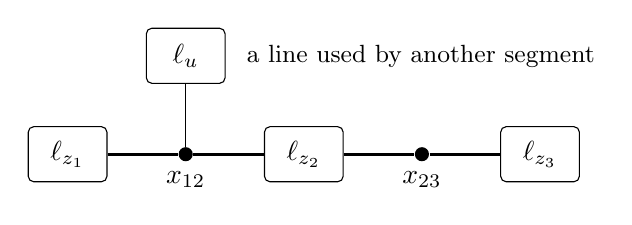
\begin{tikzpicture}[
  line vertex/.style={draw,rectangle,rounded corners=2pt,
                     minimum width=10mm,minimum height=7mm},
  point vertex/.style={circle,fill,inner sep=1.8pt}]
\node[line vertex] (l1) at (0,0) {$\ell_{z_1}$};
\node[point vertex,label=below:$x_{12}$] (p1) at (1.5,0) {};
\node[line vertex] (l2) at (3,0) {$\ell_{z_2}$};
\node[point vertex,label=below:$x_{23}$] (p2) at (4.5,0) {};
\node[line vertex] (l3) at (6,0) {$\ell_{z_3}$};
\node[line vertex] (l4) at (1.5,1.25) {$\ell_{u}$};
\draw[very thick] (l1)--(p1)--(l2)--(p2)--(l3);
\draw (p1)--(l4);
\node[anchor=west,font=\small] at (2.15,1.25)
  {a line used by another segment};
\end{tikzpicture}
\caption{A schematic incidence forest. Boxes are line vertices and dots
are projected transition points. The bold path is determined by its
two endpoint line vertices and recovers the run-label sequence
$z_1,z_2,z_3$. Edges represent incidence in the quotient space.}
\label{fig:q-forest-incidence}
\end{figure}

We describe explicitly a code for the whole column pattern.
\begin{enumerate}
\item Record imperfect positions, block boundaries, run boundaries,
and the omitted or regular status of each run.  These are binary
data on $O(k)$ positions and have $\exp(O(k))$ possibilities.
\item Record the equality partition among the omitted run-entries.
Its cost is at most $(2k)^{O(rB)}$.
\item Give the abstract forest, rooted and ordered in any manner,
with its line or point vertex types.  The parenthesis traversal of
a rooted ordered forest with at most $4k$ vertices, together with
the type bits, has $\exp(O(k))$ possibilities.  The traversal numbers
its vertices.
\item Give the ordered pair of line-vertex numbers for every regular
segment.  By the unique-path property this recovers its run sequence.
The cost is at most $(4k)^{O((2r+1)B)}$.
\item At every imperfect position, give a representative occurrence
of its label.  A label already represented in a perfect position
points to such a position; otherwise use its first imperfect
occurrence.  This costs at most $(2k)^I$.
\end{enumerate}
These data determine a unique equality partition.  Omitted labels
cannot equal regular labels.  Their recorded partition determines
all omitted equalities, while the forest vertices determine all
regular equalities.  The last step supplies every remaining equality.
Neither coordinates of transition points nor numerical coefficients
are needed in this decoding.

All constants in these code counts are absolute.  Their logarithms
sum to at most
\[
 C_0k+C_0L^{0.92}\log(4k)
       +C_0(S_1+U)\log(2k)\le Ck
\]
for an absolute $C$ and sufficiently large absolute $L$.  Here
$k=\lfloor L\rfloor$ and both exponents $0.92$ and $1/4$ are
strictly less than one.

The code universe just described depends only on the length and
the displayed numerical bounds.  Every realizable pattern, whatever
the coefficients, has a code in that same universe.  For example,
choose the first valid code in a fixed ordering; the decoder shows
that two different patterns cannot receive the same code.  Thus the
bound counts the union over all coefficients, not just the patterns
at one fixed coefficient choice.  Applying this universal bound in
each of the $J$ columns proves the last assertion.
\end{proof}

\subsection{Summing padding in a fixed residue environment}

The forest code has removed the dependence of the pattern count on
padding.  We can now sum all padding choices, keeping the departure
cut that bounds their mass at each site.  This summation uses one
shared residue environment; no independence between translated sites
is asserted.

\begin{lemma}[Padding sum]\label{q:padding-sum}
Fix an integer $m\ge1$, a bin $j$, tuples
$d_1,\ldots,d_m\in\mathcal D$, signs
$\varepsilon_1,\ldots,\varepsilon_m\in\{-1,1\}$, an initial site, and the entire
non-$P$ residue environment.  With successive sites defined by
$n_{i+1}=n_i+\varepsilon_i hq_i d_i$, one has
\begin{equation}\label{q:padding-product}
 \sum_{q_1,\ldots,q_m\in\mathcal Q}
 \prod_{i=1}^m
 \frac{Lu(q_i)}{w(n_i)}\1_{q_i\mid n_i}
 \1_{(d_i,q_i)\in\mathcal S_j}
 \1_{\rho_j(n_i,d_i)\le K/L}
 \le K^m.
\end{equation}
The bound is uniform over the fixed data and initial site.
\end{lemma}

\begin{proof}
Let $c_i(n,q)$ denote the $i$th factor in the product.  The definition
of $\rho_j$ allows all squarefree padding products in the bin; the
extra bound on $\omega(q)$ in $\mathcal S_j$ only reduces their sum.
Consequently, at every site $n$,
\[
 \sum_q c_i(n,q)
 \le L\rho_j(n,d_i)\1_{\rho_j(n,d_i)\le K/L}\le K.
\]
Set $F_{m+1}(n)=1$ and recursively define
\[
 F_i(n)=\sum_q c_i(n,q)
             F_{i+1}(n+\varepsilon_i hqd_i).
\]
Backward induction, using a bound uniform in the starting site at
each stage, gives $F_i(n)\le K^{m-i+1}$.  In particular
$F_1(n_1)\le K^m$.  The shifts caused by earlier padding choices
therefore introduce no additional factor.
\end{proof}

\subsection{Completion of the trace estimate}\label{q:trace-completion}

\begin{proof}[Proof of \Cref{q:trace}]
First work in the product residue law.  The contributions with
$U>L^{1/50}$, with a high-rank column, or with $S_1>L^{1/4}$ are
$o(1)$ in total by \Cref{q:many-unlit,q:rank,q:singletons}, including
the external dimension factors of the trace expansion.  We sum the
remaining contributions using \Cref{q:mixed-difference}.

By \Cref{q:forest-code}, the combined column patterns lie in a single
family of at most $\exp(CJk)$ possibilities, independently of all
padding choices.  Fix one such pattern, its numerical column labels,
the signs, and the lit or unlit designations.  Replace
$|\Delta G|$ by $2^{S_1}$ and retain just one reciprocal per distinct
column prime in $b_{\mathcal L}$.  Every nonsingleton provides at
least one such reciprocal: either it has a lit occurrence, or all
of its at least two occurrences are unlit.  Dropping the other
reciprocals and lit consistency enlarges the nonnegative majorant.

In $R$, drop closure, progression and block restrictions, arrival
cuts, and the low-$Q$ cuts.  Retain the padding divisibilities, bin
conditions, departure weights, and departure $\rho_j$ cuts.  The
closed-word identity for its denominators was established before
this enlargement.  Conditional on the non-$P$ environment,
\Cref{q:padding-sum} with $m=2k$ bounds the full padding sum by
$K^{2k}$.  All its factors are unchanged by the $P$-coordinate
overwrites, and the bound is uniform in the environment.  Taking
its expectation preserves that bound.

Let $m_i$ be the number of distinct labels in column $i$, and put
$m_P=\sum_i m_i$.  Among the $2kJ$ column occurrences, exactly $S_1$
belong to singleton labels and every other label occurs at least
twice.  Hence
\[
 2kJ\ge S_1+2(m_P-S_1),\qquad
 m_P\le Jk+S_1/2.
\]
After the uniform padding bound, the numerical label sum is at most
\begin{equation}\label{q:column-mass}
 \prod_{i=1}^J V_i^{m_i}
 \le (2W)^{Jk+S_1/2}
 \le (2W)^{Jk+L^{1/4}/2}.
\end{equation}
Here dropping distinctness among prime classes is simply an
enlargement of a positive reciprocal sum.  The classes are already
identified by their first occurrences, so no further permutation
factor is introduced.

There are at most $2^{2k}$ sign choices and $2^{2kJ}$ lit or unlit
designations.  The mixed difference contributes $2^{S_1}$.  The
external indices cost at most $|\mathcal D|^2M\le\exp(108L)$ for
large $L$, since $|\mathcal D|\le e^{2L}$ and
$M=\lceil e^{103L}\rceil$.  Combining these bounds with the forest
count and \eqref{q:column-mass} gives
\begin{equation}\label{q:trace-preconstant}
 \E\|H^k\|_{\mathrm{HS}}^2
 \le K^{2k}\exp(C_4Jk)(2W)^{Jk+L^{1/4}/2}+o(1),
\end{equation}
where $C_4$ is absolute.  The factor $\exp(108L)$ is absorbed here
using $J\ge1$ and $k\ge L/2$.

For every fixed $W$, once $L$ is sufficiently large,
$(2W)^{L^{1/4}/2}\le e^k$.  This changes the required lower threshold
on $L$, but not the absolute constant in the exponential.  An
absolute choice of $C_2$ therefore bounds the right-hand side of
\eqref{q:trace-preconstant} by
\[
 \bigl[K(C_2\sqrt W)^J\bigr]^{2k}.
\]
Finally, the finite-law comparison for the trace expansion changes
the expectation by at most $\exp(-L^9)$.  Increasing the same
absolute constant $C_2$ absorbs this error as well and proves the
integer-interval assertion of \Cref{q:trace}.  In particular,
$C_2$ is fixed before $W$ is selected; dependence on the fixed
parameters is confined to how large $X$ must be.
\end{proof}

\section{Spectral transfer and the bound at every scale}
\label{q:sec-spectral}

The moment bound for $H$ has only square-root dependence on each
prime supply's reciprocal mass. We now use it to control the retained
centered sums $C_j^\circ$. First we transfer control of $H$ to the
projected edge operator $E(\sum_d A_d)E$, then test against the
Liouville function with vertex weight $\sqrt w$. The factor $L$ in
the edge matrices yields a factor $1/L$ in the estimate for each bin,
compensating for the factor $L$ in the number $O(L/\eta)$ of bins.
After division by the retained mass $S_0\ge SV_*/2$, with $V_*\ge W^J$,
the spectral contribution will have the form
\[
 \frac K\eta\left(\frac C{\sqrt W}\right)^J
\]
for an absolute constant $C$. We prove the transfer and the required
finite-interval estimates before choosing $W$.

The use of a nonbacktracking operator to control an adjacency operator
is exemplified by the weighted Ihara--Bass formula in
\cite[Section~4.2]{Pilatte26}.  We prove the transfer needed here
directly for self-adjoint edge operators; distinct edge operators need
not commute.

\subsection{A transfer lemma for self-adjoint edge matrices}

\begin{lemma}\label{q:noncommuting}
Let $N\ge1$ and let $B_1,\ldots,B_N$ be self-adjoint operators on a finite-dimensional
complex Hilbert space $\mathcal H$, and let $P$ be an orthogonal
projection on $\mathcal H$. Define an operator $\mathscr B$ on
$\mathcal H^N$ by
\[
 \mathscr B_{i,j}=\1_{i\ne j}B_j.
\]
Suppose $a,b\ge0$, $\|B_i\|\le a$ for every $i$, and
\[
 \sum_{i=1}^N\|B_i v\|^2\le b^2\|v\|^2
 \qquad(v=Pv).
\]
Writing $\rho(\mathscr B)$ for its spectral radius, one has
\begin{equation}\label{q:noncommuting-bound}
 \left\|P\left(\sum_{i=1}^N B_i\right)P\right\|
 \le 3\max\{a,b,\rho(\mathscr B)\}.
\end{equation}
\end{lemma}

\begin{proof}
Put $m=\max\{a,b,\rho(\mathscr B)\}$. If $m=0$, all $B_i$ vanish.
Otherwise set $t=(2m)^{-1}$. For real $|u|\le t$, the operators
$I-u\mathscr B$ and $I+uB_i$ are invertible. Define
\[
 F(u)=I-\sum_{i=1}^N uB_i(I+uB_i)^{-1}.
\]
Each summand is self-adjoint, since $B_i$ commutes with its own
resolvent. If $F(u)v=0$, set $z_i=(I+uB_i)^{-1}v$. Then
\[
 (u\mathscr Bz)_i
 =\sum_{j\ne i}uB_jz_j
 =v-uB_i z_i=z_i.
\]
A nonzero $v$ would give a nonzero $z$, contradicting the invertibility
of $I-u\mathscr B$. Hence $F(u)$ is invertible throughout $[-t,t]$.
It is positive definite there by continuity, because $F(0)=I$.

The resolvent identity gives
\[
 F(u)=I-u\sum_i B_i+Q(u),\qquad
 Q(u)=u^2\sum_i B_i^2(I+uB_i)^{-1}.
\]
Since $|u|\|B_i\|\le1/2$, the inverses in the last expression are
positive and bounded above by $2I$. For $v=Pv$,
\[
 0\le\langle v,Q(u)v\rangle
 \le2u^2\sum_i\|B_i v\|^2
 \le2u^2b^2\|v\|^2.
\]
Positivity of $F(t)$ and $F(-t)$ therefore yields
\[
 \left|\left\langle v,\sum_i B_i v\right\rangle\right|
 \le \frac{1+2t^2b^2}{t}\|v\|^2
 \le3m\|v\|^2.
\]
Taking the supremum over unit vectors in the range of $P$ proves
\eqref{q:noncommuting-bound}. No step commutes two distinct $B_i$.
\end{proof}

\subsection{Weighted row bounds and the degree projection}

Fix a bin $j$ and one block of $M$ sites, with its matrices $A_d$, $H$
and projection $E$ from the trace construction. Define
\[
 a_d(n)=\prod_{p\mid d}\left|\1_{p\mid n}-\frac1p\right|.
\]
If $A_d(n,n')\ne0$, the difference $n'-n$ is a multiple of $d$.
Thus $a_d(n)=a_d(n')$ along every edge of $A_d$.

\begin{lemma}\label{q:weighted-rows}
On every block, in either the product model or the integer model,
\begin{align}
 \|A_d\|&\le2K,\label{q:single-operator}\\
 \sum_{d\in\mathcal D}\|A_d v\|^2
 &\le4K^2(8W)^J\|v\|^2\qquad(v=Ev).
 \label{q:square-operators}
\end{align}
\end{lemma}

\begin{proof}
For each of the two edge orientations, the weighted absolute row sum
at $n$ is at most
\[
 a_d(n)\sum_q\frac{Lu(q)}{w(n)}\1_{q\mid n}
 \1_{(d,q)\in\mathcal S_j}\1_{\rho_j(n,d)\le K/L}
 \le K a_d(n).
\]
Indeed the sum without the last indicator is at most
$L\rho_j(n,d)$. For an incoming edge, $q$ divides one endpoint if
and only if it divides the other. All the other edge restrictions can
be discarded in this nonnegative bound. Consequently
\begin{equation}\label{q:weighted-row}
 \sum_{n'}|A_d(n,n')|
       \frac{\sqrt{w(n')}}{\sqrt{w(n)}}\le2K a_d(n).
\end{equation}

The weighted Schur inequality for a real symmetric matrix $B$ follows
by applying
\[
 2|v_n v_{n'}|\le
 |v_n|^2\frac{\sqrt{w(n')}}{\sqrt{w(n)}}+
 |v_{n'}|^2\frac{\sqrt{w(n)}}{\sqrt{w(n')}}
\]
to its quadratic form. Apply it to $A_d$ on each level set of $a_d$;
these level sets are invariant under $A_d$. The resulting bound is
\begin{equation}\label{q:localized-square}
 \|A_d v\|^2\le4K^2\sum_n a_d(n)^2|v_n|^2.
\end{equation}
In particular, $a_d(n)\le1$ proves \eqref{q:single-operator}.

At a site retained by $E$, the total P-degree is at most $6WJ$.
Since $V_i\le2W$, the arithmetic-geometric mean inequality gives
\begin{align*}
 \sum_d a_d(n)^2
 &\le\sum_d a_d(n)
 \le\prod_{i=1}^J\bigl(\omega_{P_i}(n)+V_i\bigr)\\
 &\le\left(\frac{\omega_P(n)+\sum_iV_i}{J}\right)^J
 \le(8W)^J.
\end{align*}
Sum \eqref{q:localized-square} over $d$. This proves
\eqref{q:square-operators} without requiring $E$ to commute with $A_d$.
\end{proof}

\begin{proposition}\label{q:spectral}
There is an absolute constant $C_3$ with the following property.
For each bin $j$, average block origins over any integer interval to
which \Cref{q:trace} applies. Outside a fraction at most $e^{-2k}$ of
these origins,
\begin{equation}\label{q:compressed-norm}
 \left\|E\left(\sum_d A_d\right)E\right\|
 \le K(C_3\sqrt W)^J.
\end{equation}
\end{proposition}

\begin{proof}
For every finite matrix, $\rho(H)^{2k}\le\|H^k\|_{\mathrm{HS}}^2$.
Thus \Cref{q:trace} and Markov's inequality show that
\[
 \rho(H)\le eK(C_2\sqrt W)^J
\]
except on a fraction at most $e^{-2k}$ of the origins. On each remaining
block apply \Cref{q:noncommuting} with
\[
 a=2K,\qquad b=2K(8W)^{J/2},\qquad P=E.
\]
For $J\ge1$ and $W\ge10$, the choice
\begin{equation}\label{q:C3-choice}
 C_3=3\max\{2,2\sqrt8,eC_2\}
\end{equation}
gives \eqref{q:compressed-norm}. In particular, $C_3$ is independent of
$W,h,l$.
\end{proof}

\subsection{Testing and averaging overlapping blocks}

We now turn \eqref{q:compressed-norm} into an estimate for $C_j^\circ$,
the retained correlation in \Cref{q:cuts}. Its endpoint restrictions
are exactly those imposed by the $A_d$ and the projection $E$.

\begin{proposition}\label{q:testing}
For every bin $j$ and all sufficiently large $X$,
\begin{equation}\label{q:bin-estimate}
 |C_j^\circ|\ll \frac{S K(C_3\sqrt W)^J}{L}+e^{-L}.
\end{equation}
The threshold may depend on the fixed $h,l,W$, while $C_3$ is the
absolute constant in \eqref{q:C3-choice}.
\end{proposition}

\begin{proof}
Write $T=T_j$ and $N=\lfloor T\rfloor$, and average over blocks
$I_t=\{t+1,\ldots,t+M\}$, $0\le t<N$. For large $X$,
$N\ge\exp(L^A/2)$, so the interval of origins is admissible in
\Cref{q:finite-law,q:trace}. On each block put
\[
 f_t(n)=\sqrt{w(n)}\lambda(n)
             \1_{\omega_Q(n)\le400\log L},\qquad g_t=Ef_t.
\]
We first check the averaged norm needed for testing:
\begin{equation}\label{q:test-vector-norm}
 \frac1N\sum_{t=0}^{N-1}\|g_t\|^2
 \le\frac1N\sum_{t=0}^{N-1}\|f_t\|^2\le2MS.
\end{equation}
For each of the $M$ block positions, \Cref{q:truncated-weight}
applied to the corresponding translated interval of $N$ origins
bounds the average truncated weight by $2S$. Summing proves
\eqref{q:test-vector-norm}. This uses the truncated comparison
already established, without an untruncated integer moment of $w$.

On blocks satisfying \eqref{q:compressed-norm}, the averaged absolute
quadratic form is at most $2MSK(C_3\sqrt W)^J$. On every block,
including exceptional ones, \eqref{q:weighted-row} gives the
deterministic bound
\begin{equation}\label{q:deterministic-test}
 \left|\left\langle g_t,\sum_d A_d g_t\right\rangle\right|
 \le 2KM\,5^{400\log L}(8W)^J.
\end{equation}
Here we bound the form by its entrywise absolute value, use
$|g_t(n)|\le\sqrt{w(n)}$, and then sum the weighted row bounds at
sites satisfying both degree cutoffs. The right side divided by $M$
is a fixed power of $L$ for fixed $W$. Multiplication by the exceptional
fraction $e^{-2k}$ makes its contribution, after division by $2LM$,
at most $e^{-L}$ for large $L$. Therefore
\begin{equation}\label{q:averaged-form}
 \left|\frac1{2LMN}\sum_{t=0}^{N-1}
       \left\langle g_t,\sum_d A_d g_t\right\rangle\right|
 \ll \frac{S K(C_3\sqrt W)^J}{L}+e^{-L}.
\end{equation}

It remains to compare this form with the original prefix sum. Denote
by $c_j(n;d,q)$ the signed summand belonging to $(d,q)$ in
$T C_j^\circ$, including all its endpoint cutoffs. Use the same
formula to define it for every positive $n$, and put $r=hqd$. These cutoffs
are predicates of the ambient sites, independent of the choice of
block; restricting to a block only removes edges leaving it.
Testing an increasing matrix entry cancels its two square-root
weights and gives $L c_j(n;d,q)$; symmetry gives the same term in the
opposite orientation. Thus the form on the left of
\eqref{q:averaged-form}, before taking absolute values, is exactly
\begin{equation}\label{q:edge-multiplicity}
 \frac1{MN}\sum_{n,d,q}m_N(n,r)c_j(n;d,q),\qquad
 m_N(n,r)=
 \bigl[\min(N-1,n-1)-\max(0,n+r-M)+1\bigr]_+,
\end{equation}
where $[x]_+=\max(x,0)$. This is the number of blocks containing both
endpoints. All contributing $n$ are positive.

Let
\[
 R_L=h e^{100L+1},\qquad
 D_L=\frac KL\,5^{400\log L}(8W)^J.
\]
Every displacement is at most $R_L$, and the one-orientation row
bound proves $\sum_{d,q}|c_j(n;d,q)|\le D_L$ for every $n$.
For large $L$ we have $N\gg M>R_L$. If $M\le n\le N$, then
$m_N(n,r)=M-r$. The lower boundary and the extra sites $N<n<N+M$
contain at most $2M$ sites, and always $0\le m_N(n,r)\le M$.
Consequently the difference between \eqref{q:edge-multiplicity} and
$C_j^\circ=T^{-1}\sum_{n\le N,d,q}c_j(n;d,q)$ is at most
\begin{equation}\label{q:prefix-error}
 O\left(D_L\left(\frac{R_L}{M}+\frac MN+\frac1T\right)\right).
\end{equation}
The last term accounts for replacing $N^{-1}$ by $T^{-1}$.
Since $M=\lceil e^{103L}\rceil$, $T\ge X=e^{L^A}$ and $D_L$ is
polynomial in $L$, \eqref{q:prefix-error} is $O(e^{-L})$ for
sufficiently large $L$. This also bounds edges whose terminal endpoint
exceeds $T$ and the floor errors. Combining with
\eqref{q:averaged-form} proves \eqref{q:bin-estimate}.
\end{proof}

\subsection{Final choice of constants}

\begin{proof}[Proof of \Cref{q:progression}]
There are $O(L/\eta)$ bins. Sum \eqref{q:bin-estimate}, use
$S_0\ge SV_*/2$ and $V_*\ge W^J$, and then apply the centering and
deletion estimates of \Cref{q:center,q:cuts}. We obtain
\begin{align}
 |F(X)|\ll_{h,l,W}{}&
 \eta+\eta^{-1}2^J L^{-1/20}
 +2^J\bigl(K^{-1}+L^{-100}+e^{-2WJ}\bigr)\notag\\
 &+\frac K\eta\left(\frac{C_3}{\sqrt W}\right)^J
 +e^{-L^{0.9}}+X^{-1}.
 \label{q:finish}
\end{align}
The deletion error in \Cref{q:cuts} is already summed over the bins.
The new error $O((L/\eta)e^{-L})$ from \Cref{q:testing} is absorbed
by $e^{-L^{0.9}}$, because $L/\eta$ is polynomial in $L$ and $SV_*\ge1$.

Choose the absolute constants in the following order. First fix $A$
as required by \Cref{q:finite-law}; in particular $A\ge1000$ and
$A>C_1+20$, where $C_1$ is the absolute exponent in that comparison.
The trace proof gives an absolute $C_2$, and
\eqref{q:C3-choice} then gives an absolute $C_3$. Now choose $W\ge10$
so large that
\begin{equation}\label{q:W-choice}
 e^5 C_3/\sqrt W\le e^{-1}.
\end{equation}
Only after fixing these constants do we increase the threshold for
$X$, allowing it to depend on $h,l,W$.

Recall $\eta=e^{-J}$, $K=e^{4J}$ and
$J\le\delta\log L/(6W)$ with $\delta=1/200$.
The spectral term in \eqref{q:finish} is at most $e^{-J}$ by
\eqref{q:W-choice}. The other terms satisfy
\begin{align*}
 2^JK^{-1}&=e^{-(4-\log2)J}\le e^{-J},\\
 2^Je^{-2WJ}&=e^{-(2W-\log2)J}\le e^{-J},\\
 e^J2^J L^{-1/20}&\le e^{-J},\qquad
 2^J L^{-100}\le e^{-J}.
\end{align*}
For the last line, it is enough to note that
\[
 \frac{\delta(2+\log2)}{6W}<\frac1{20},\qquad
 \frac{\delta(1+\log2)}{6W}<100.
\]
Also $e^{-L^{0.9}}+X^{-1}\ll e^{-J}$ for large $X$. Hence
$|F(X)|\ll_{h,l}e^{-J}$. Finally,
\[
 e^{-J}\le e L^{-\delta/(6W)}
 =e(\log X)^{-c},\qquad c=\frac{\delta}{6WA}>0.
\]
All three constants $A,W,c$ are absolute. The argument applies to
every sufficiently large real $X$, with no excluded scales. On the
remaining bounded range $3\le X\le X_0(h,l)$, the estimate follows
from $|F(X)|\le1$ after enlarging the implied constant. This proves
\Cref{q:progression}.
\end{proof}

\section{The quantitative affine bound}\label{q:affine-transfer}

The progression estimate for Liouville gives the same logarithmic
exponent for every fixed affine pair. The finite initial interval
affects only the constant.

\begin{proof}[Proof of \Cref{thm:q-affine}]
Fix $a_1,a_2\ge1$ and $b_1,b_2\ge0$ with nonzero determinant, and
put
\[
 l=a_1a_2,\qquad c_0=\min(a_2b_1,a_1b_2),\qquad
 h=|a_1b_2-a_2b_1|>0.
\]
Multiplying the two affine arguments by $a_2$ and $a_1$, respectively,
and using complete multiplicativity gives
\begin{equation}\label{q:quant-affine-identity}
 \lambda(a_1n+b_1)\lambda(a_2n+b_2)
 =\lambda(l)\lambda(ln+c_0)\lambda(ln+c_0+h).
\end{equation}
Here $\lambda(l)^2=1$. For real $Y\ge0$ set
\[
 P(Y)=\sum_{1\le m\le Y}
       \lambda(m)\lambda(m+h)\1_{m\equiv c_0\pmod l}.
\]
The sum is empty for $Y<1$. Let $c>0$ be the absolute exponent in
\Cref{q:progression}. That estimate applies to the residue $c_0$
without any coprimality restriction and gives
\[
 |P(Y)|\ll_{l,h,c_0}\frac{Y}{(\log Y)^c}\qquad(Y\ge3).
\]
For every real $X\ge3$, the integers in the class $c_0\pmod l$
with $c_0<m\le lX+c_0$ are precisely $m=ln+c_0$ with
$1\le n\le X$. Consequently \eqref{q:quant-affine-identity}
gives the exact endpoint identity
\begin{equation}\label{q:affine-rate-endpoints}
 \sum_{1\le n\le X}\lambda(a_1n+b_1)\lambda(a_2n+b_2)
   =\lambda(l)\bigl(P(lX+c_0)-P(c_0)\bigr).
\end{equation}
This identity includes both determinant signs and noninteger cutoffs.
Since $lX+c_0\ge X\ge3$ and
$lX+c_0\le(l+c_0/3)X$, the first term satisfies
\[
 |P(lX+c_0)|
 \ll_{a_1,a_2,b_1,b_2}\frac{X}{(\log X)^c}.
\]
Also $|P(c_0)|\le c_0$, which is absorbed into the same bound:
the function $(\log X)^c/X$ is bounded on $[3,\infty)$.
The exponent has not changed and is independent of the affine
coefficients; only the implied constant depends on them. This proves
\Cref{thm:q-affine} for all real $X\ge3$.
\end{proof}

\part{Qualitative correlations of general multiplicative functions}
\noindent
We now prove \Cref{thm:elliott}. The graph in this part uses a different
normalization and a different order of limits. Its parameters and prime
sets are defined afresh; none of the choices of \(A,W,L,J,\eta\) in
Part~I is in force here. The functions and their nonpretentiousness
condition remain those of the introduction.
\section{The weighted divisor graph}\label{sec:graph-setup}

We begin the qualitative argument with the finite-scale graph estimate
that will rule out a correlation bias. Its test functions are arbitrary bounded sequences;
no multiplicativity enters its statement or proof. The arithmetic
application follows in \Cref{sec:analytic-transfer}.

Fix an integer $h\ge1$. Throughout the graph construction use
\begin{equation}\label{eq:graph-constants}
 \eps=10^{-4},\quad \eta=\eps/100,\quad \rho=1/20,\quad
 \kappa=400/\eta,\quad A=\exp(2\kappa),\quad c_*=\eps/100.
\end{equation}
The scale $B$ will be sufficiently large. Define two finite prime sets by
\begin{equation}\label{eq:prime-bands}
 \begin{split}
 \mathcal C&=\{p:B^{1-\eta}<\log p\le B\},\\
 \mathcal Z&=\{p:B^{1-\eps}<\log p\le B^{1-\eta}\},\qquad
 \mathcal S=\mathcal C\cup\mathcal Z,\quad P_0=\exp(B^{1-\eps}).
 \end{split}
\end{equation}
We refer to $\mathcal C$ as the core band and $\mathcal Z$ as the center
band. For $a\in\{C,Z\}$, set $\mathcal P_C=\mathcal C$ and
$\mathcal P_Z=\mathcal Z$, and put
\[
 v_a=\sum_{p\in\mathcal P_a}\frac1p,\qquad
 A_C=A,\quad A_Z=1,\quad \beta_a=(1+A_a)^{-1},\qquad
 \theta=\beta_Z^2=\tfrac14.
\]
Mertens' prime harmonic estimate gives
\[
 v_C=(\eta+o(1))\log B,\qquad
 v_Z=(\eps-\eta+o(1))\log B.
\]

Fix also $\tau\in(1,2)$, $C_0\ge1$, and $T>0$. An admissible divisor
family $\mathcal D$ is any collection of squarefree products of primes
in $\mathcal S$ such that
\begin{equation}\label{eq:divisor-family}
 \begin{gathered}
 d>1,\qquad H<d\le\tau H,\qquad 1\le H\le\exp(C_0B),\\
 \omega(d)\le J:=\lceil C_0\log B\rceil.
 \end{gathered}
\end{equation}
Here $\omega$ counts distinct prime factors. For any integer $x$, define
$\omega_a(x)=\#\{p\in\mathcal P_a:p\mid x\}$, and write
$d_C=\prod_{p\mid d,\ p\in\mathcal C}p$.
For each $d\in\mathcal D$, let $w_d:\Z\to[0,1]$ be any function of
all the residues $x\bmod p$, $p\in\mathcal C$, with support restricted by
\begin{equation}\label{eq:core-cutoff}
 w_d(x)=0\quad\hbox{unless}\quad
 k_d(x):=\#\{p\in\mathcal C:p\mid x,\ p\nmid d\}
       \ge v_C-T\sqrt{v_C}.
\end{equation}
The cutoff need not factor over primes.

For $y=x\pm hd$, define the real edge weight
\begin{equation}\label{eq:graph-kernel}
 g_d(x,y)=w_d(x)w_d(y)A^{\omega_C(d)}\1_{d_C\mid x}
       \prod_{\substack{p\mid d\\p\in\mathcal Z}}
             \left(\1_{p\mid x}-\frac\theta p\right).
\end{equation}
For each $p\mid d$, the residues of $x$ and $y$ agree modulo $p$.
Consequently $g_d(x,y)=g_d(y,x)$. The uncentered core factors enforce
$d_C\mid x$, whereas the center factors can have either sign.

The vertex weight and its mean are
\begin{equation}\label{eq:graph-weights}
 W(x)=\prod_{a\in\{C,Z\}}\beta_a^{-\omega_a(x)},\qquad
 L_0=\prod_{a\in\{C,Z\}}\prod_{p\in\mathcal P_a}(1+A_a/p).
\end{equation}
Let $Q_B=\prod_{p\in\mathcal S}p$. We use the uniform probability space
$\Z/Q_B\Z$, identified by the Chinese remainder theorem with the product
of the uniform spaces $\Z/p\Z$. Its expectation is denoted by $\E$;
$\E_U$ averages only coordinates indexed by $U\subseteq\mathcal S$.
For a uniform residue $n$,
\begin{equation}\label{eq:weight-moments}
 \E W(n)=L_0,\qquad
 \E W(n)^2
 =\prod_a\prod_{p\in\mathcal P_a}
        \left(1+\frac{\beta_a^{-2}-1}{p}\right)
 \le \exp\bigl((A^2+2A)v_C+3v_Z\bigr)=B^{O_A(1)}.
\end{equation}
Both identities follow by independence of the prime coordinates.
The exponent in the last bound is fixed, although large.

\begin{proposition}[Divisor graph estimate]\label{prop:graph-estimate}
Fix $h\ge1$, $1<\tau<2$, $C_0\ge1$, and $T>0$, and use
\eqref{eq:graph-constants}--\eqref{eq:graph-weights}. For every sufficiently
large $B$, every admissible family $\mathcal D$, all permitted cutoffs
$w_d$, all coefficients $|a_d|\le1$, and all functions
$F,G:\N\to\mathbb D$,
\begin{equation}\label{eq:graph-estimate}
 \limsup_{X\to\infty}\frac1X
 \left|\sum_{1\le x\le X}\sum_{d\in\mathcal D}
 a_dF(x)G(x+hd)g_d(x,x+hd)\right|
 \ll L_0 B^{-1-c_*/2}.
\end{equation}
The implied constant and the threshold for $B$ may depend on
$h,\tau,C_0,T$, and the fixed constants in \eqref{eq:graph-constants},
but not on $H,\mathcal D,w_d,a_d,F,G$. All graph parameters are fixed
when $X$ tends to infinity.
\end{proposition}

The proof occupies \Cref{sec:paths,sec:thinning,sec:cylinder-sieve,sec:trace-count,sec:localization}.
The two bands have different roles in that proof. The core weights and
cutoffs give savings from the short divisor interval and from the
lower bound on $k_d(x)$ in \eqref{eq:core-cutoff}.
The center factors provide further cancellation in closed-walk products,
where each edge weight is divided by $W$ at its starting vertex.
The relation $\theta=\beta_Z^2$ matches the
centering constant to that normalization; its precise use is established
in \Cref{sec:trace-count}, once the relevant walk configurations have
been defined.

The comparison scale is $L_0/B$. In the next section, one of $O(B)$
short multiplicative intervals captures enough divisor weight to turn
any persistent correlation bias into a sum of this size with ordinary
divisibility indicators. The extra factor $B^{-c_*/2}$ in
\eqref{eq:graph-estimate} will contradict that
bias once the analytic cost of centering has been bounded.

\section{Reduction to the graph estimate}\label{sec:analytic-transfer}

We now explain how \Cref{prop:graph-estimate} rules out a nonzero
multiplicative correlation. The first step produces a large sum with
ordinary divisibility indicators. We then state the estimate that permits
centering those indicators, and display the resulting contradiction.
The proof of the centering estimate occupies
\Cref{sec:analytic-centering}; the graph estimate itself will be proved
in \Cref{sec:localization}.

\subsection{Absolute-value defects and a biased sequence}

A multiplicative function satisfies $f(1)=f(1)^2$. If $f(1)=0$, then
$f(n)=f(n)f(1)=0$ for every $n$. We may therefore suppose that both
functions in \Cref{thm:elliott} take the value $1$ at $1$.
There is another case in which the conclusion follows without a graph.

\begin{lemma}\label{lem:analytic-absolute-defect}
Let $f\colon\N\to\C$ be multiplicative and $|f|\le1$. If
\[
 \sum_p\frac{1-|f(p)|}{p}=\infty,
\]
then $N^{-1}\sum_{n\le N}|f(n)|\to0$.
\end{lemma}
\begin{proof}
Write $v_p(n)$ for the exponent of $p$ in $n$. For a finite set
$\mathcal P$ of primes, multiplicativity gives
\[
 |f(n)|\le
 \prod_{\substack{p\in\mathcal P\\v_p(n)=1}}|f(p)|.
\]
The majorant is periodic modulo $\prod_{p\in\mathcal P}p^2$.
Its ordinary mean is
\[
 \prod_{p\in\mathcal P}
 \left(1-(1-|f(p)|)\left(\frac1p-\frac1{p^2}\right)\right).
\]
These products tend to zero as $\mathcal P$ increases through the primes:
the sum of the subtracted quantities diverges, whereas
$\sum_p p^{-2}<\infty$. First take the long average with $\mathcal P$
fixed, and then increase $\mathcal P$.
\end{proof}

A fixed translation affects only finitely many terms of a bounded
average. Thus, after translating by the smaller shift and ordering the
functions accordingly, it suffices to prove cancellation of
$f_1(m)f_2(m+h)$ for a fixed $h\ge1$.
By \Cref{lem:analytic-absolute-defect}, we may assume
\begin{equation}\label{eq:analytic-finite-defects}
 \sum_p\frac{1-|f_i(p)|}{p}<\infty\qquad(i=1,2).
\end{equation}
If the desired cancellation fails, there are $0<\gamma\le1$ and positive
integers $N_j\to\infty$ such that
\begin{equation}\label{eq:analytic-bias}
 \left|S(N_j)\right|\ge\gamma N_j,
 \qquad S(N)=\sum_{m\le N}f_1(m)f_2(m+h).
\end{equation}
We retain this same sequence throughout the argument.
The numbers $S(N_j)$ may have varying complex arguments.

Fix $1<\tau<2$ sufficiently close to $1$ in terms of $\gamma$, and then
fix $T$ sufficiently large in terms of $\gamma$. Choose
$\phi\in C_c^\infty(\R)$ with $0\le\phi\le1$, supported in $[-T,T]$
and equal to $1$ on $[-T/2,T/2]$. For every admissible divisor $d$, use
\begin{equation}\label{eq:analytic-cutoffs}
 w_d(x)=\phi\left(\frac{k_d(x)-v_C}{\sqrt{v_C}}\right).
\end{equation}
These cutoffs satisfy the support and residue-dependence requirements
of \Cref{prop:graph-estimate}.

\subsection{Capturing the bias in one divisor interval}

Recall that $\mathcal S=\mathcal C\cup\mathcal Z$ is the finite prime set
at scale $B$, and that a squarefree product $d$ of these primes has
weight $A^{\omega_C(d)}$. The normalizing factor $L_0$ has the exact
expansion
\begin{equation}\label{eq:raw-divisor-law}
 L_0=\sum_{\substack{d\ \mathrm{squarefree}\\p\mid d\Rightarrow p\in\mathcal S}}
       \frac{A^{\omega_C(d)}}d.
\end{equation}
The term $d=1$ is included here.

\begin{lemma}[A divisor interval carrying positive mass]
\label{lem:raw-bin}
Let $f_1,f_2\colon\N\to\C$ be $1$-bounded multiplicative functions
satisfying \eqref{eq:analytic-finite-defects} and $f_1(1)=f_2(1)=1$.
Fix $1<\tau<2$. There are constants $C_0\ge1$ and
$c>0$ such that, for every sufficiently large $B$, one can choose
$1\le H\le\exp(C_0B)$ and a family $\mathcal D$ of squarefree
$\mathcal S$-products satisfying
\begin{gather}
 H<d\le\tau H,\qquad d>1,\qquad
 \omega(d)\le J=\lceil C_0\log B\rceil,
 \qquad |f_1(d)f_2(d)|\ge\tfrac12,
 \label{eq:raw-selected-divisors}\\
 \sum_{d\in\mathcal D}\frac{A^{\omega_C(d)}}d
 \ge c\frac{L_0}{B}.
 \label{eq:raw-bin-mass}
\end{gather}
The constants are independent of $B$ and of the long averaging variable.
\end{lemma}
\begin{proof}
Normalize the summands of \eqref{eq:raw-divisor-law} to a probability
law on divisors, and denote its expectation and probability by
$\E_{\mathrm{div}}$ and $\Pbb_{\mathrm{div}}$. Each prime $p$ in band $a$
is included independently with
probability $A_a/(p+A_a)$. Prime harmonic estimates give
\[
 \E_{\mathrm{div}}\omega(d)\ll_A\log B,
 \qquad
 \E_{\mathrm{div}}\log d\le A\sum_{p\le e^B}\frac{\log p}{p}\ll_A B.
\]
Choose $C_0$ large enough that the probabilities of
$\omega(d)>\lceil C_0\log B\rceil$ and $\log d>C_0B$ are each at most
$1/8$, by Markov's inequality.

For $r_p=|f_1(p)f_2(p)|$, the inequality
$1-\prod_j r_j\le\sum_j(1-r_j)$, valid when $0\le r_j\le1$, gives
\begin{align*}
 \E_{\mathrm{div}}\bigl(1-|f_1(d)f_2(d)|\bigr)
 &\le A\sum_{p>P_0}\frac{1-|f_1(p)f_2(p)|}{p}\\
 &\le A\sum_{p>P_0}\frac{(1-|f_1(p)|)+(1-|f_2(p)|)}p=o(1).
\end{align*}
Here squarefreeness permits the use of multiplicativity.
Another application of Markov's inequality shows that the probability
of $|f_1(d)f_2(d)|<1/2$ tends to zero. Also
$\Pbb_{\mathrm{div}}(d=1)=L_0^{-1}\to0$.
Thus the remaining divisors carry at least $L_0/2$ of the unnormalized
mass for large $B$.

There are at most $1+C_0B/\log\tau$ intervals
$(\tau^r,\tau^{r+1}]$, $r\ge0$, meeting $(1,e^{C_0B}]$.
One of them carries at least $cL_0/B$ of that mass, for a fixed $c>0$.
Take its lower endpoint as $H$ and retain the divisors already satisfying
the preceding conditions.
\end{proof}

For any such divisor family, any coefficients $|a_d|\le1$, and the
cutoffs \eqref{eq:analytic-cutoffs}, define the raw and centered sums by
\begin{align}
 R_B(X)&=\sum_{x\le X}\sum_{d\in\mathcal D}
 a_d A^{\omega_C(d)}f_1(x)f_2(x+hd)
 w_d(x)w_d(x+hd)\1_{d\mid x},
 \label{eq:raw-sum}\\
 C_B(X)&=\sum_{x\le X}\sum_{d\in\mathcal D}
 a_df_1(x)f_2(x+hd)g_d(x,x+hd).
 \label{eq:analytic-centered-sum}
\end{align}
The first sum retains ordinary divisibility by all primes of $d$;
the second is the sum bounded by \Cref{prop:graph-estimate}.

\begin{lemma}[Raw lower bound]\label{lem:raw-lower-bound}
Let $f_1,f_2\colon\N\to\C$ be $1$-bounded multiplicative functions,
with $f_1(1)=f_2(1)=1$, satisfying \eqref{eq:analytic-bias} and
\eqref{eq:analytic-finite-defects}. Choose $1<\tau<2$ and $T>0$ with
$\tau-1\le\gamma/64$ and $32/T^2\le\gamma/64$, and use a cutoff
$\phi$ as in \eqref{eq:analytic-cutoffs}, equal to $1$ on
$[-T/2,T/2]$. With $\mathcal D,H$ supplied by \Cref{lem:raw-bin}, set
\[
 a_d=\overline{f_1(d)f_2(d)},\qquad X_j=HN_j.
\]
There is $c_\gamma>0$, independent of $B,j$, such that, for every
sufficiently large fixed $B$,
\begin{equation}\label{eq:raw-lower-bound}
 \liminf_{j\to\infty}\frac{|R_B(X_j)|}{X_j}
 \ge c_\gamma\frac{L_0}{B}.
\end{equation}
\end{lemma}
\begin{proof}
Put
\[
 V_{\mathcal D}=\sum_{d\in\mathcal D}A^{\omega_C(d)},\qquad
 K_{\mathcal D}=\sum_{d\in\mathcal D}
   |f_1(d)f_2(d)|^2A^{\omega_C(d)}\ge\tfrac14 V_{\mathcal D}.
\]
For a fixed $d$, write $x=dm$. Unless
$\gcd(d,m)>1$ or $\gcd(d,m+h)>1$, ordinary multiplicativity gives
\[
 a_df_1(dm)f_2(d(m+h))
   =|f_1(d)f_2(d)|^2f_1(m)f_2(m+h).
\]
The exceptional set has ordinary density at most
$2\sum_{p\mid d}p^{-1}\le2J/P_0$. At fixed $B$ there are only finitely
many $d$, so all associated residue-counting errors vanish as
$j\to\infty$.

For $p\in\mathcal C$ not dividing $d$, divisibility of $dm$ by $p$ is
equivalent to divisibility of $m$. Hence the mean and variance of
$k_d(dm)$ under uniform residues are
\[
 \mu_d=v_C-\sum_{\substack{p\mid d\\p\in\mathcal C}}\frac1p,
 \qquad
 \operatorname{Var}(k_d(dm))
 =\sum_{\substack{p\in\mathcal C\\p\nmid d}}
       \frac1p\left(1-\frac1p\right)\le v_C.
\]
The same formulas hold with $m+h$ in place of $m$. For large $B$,
$|\mu_d-v_C|\le J/P_0\le(T/4)\sqrt{v_C}$. Chebyshev's inequality and
a union bound show that the proportion on which either cutoff is not
$1$ is at most $32/T^2$. Independence of the two endpoints is not needed.

The length $X_j/d$ lies between $N_j/\tau$ and $N_j$. Comparing each
shorter sum with the sum up to $N_j$ therefore gives
\begin{equation}\label{eq:raw-comparison}
 \begin{split}
 |R_B(X_j)-K_{\mathcal D}S(N_j)|
 \le N_jV_{\mathcal D}\left(
 \tau-1+\frac{32}{T^2}+\frac{4J}{P_0}+o_{j\to\infty}(1)\right).
 \end{split}
\end{equation}
The factor $4J/P_0$ allows a difference of size at most $2$ on each
coprimality failure. The endpoint rounding errors are included in $o(1)$.

Choose $\tau-1\le\gamma/64$ and $32/T^2\le\gamma/64$, and then take
$B$ and $j$ large enough for the other two errors to be at most
$\gamma/64$ each. The reverse triangle inequality, valid for the
complex number $S(N_j)$, yields
\[
 |R_B(X_j)|\ge\frac\gamma8N_jV_{\mathcal D}.
\]
Finally,
$V_{\mathcal D}\ge H\sum_{d\in\mathcal D}A^{\omega_C(d)}/d
\ge cHL_0/B$. This proves the result with $c_\gamma=\gamma c/8$.
\end{proof}

\subsection{The centering estimate and the contradiction}

The remaining analytic task is to show that centering changes the raw
sum by less than its lower bound. Its statement does not require
\eqref{eq:analytic-finite-defects}.

\begin{proposition}[Analytic centering estimate]
\label{prop:analytic-centering}
Let $f_1,f_2\colon\N\to\C$ be multiplicative, with $|f_i|\le1$, and
suppose at least one is uniformly nonpretentious. Fix
$h\ge1$, $1<\tau<2$, $C_0\ge1$, $T>0$, and a smooth function
$0\le\phi\le1$ supported in $[-T,T]$.
For each sufficiently large $B$, let $\mathcal D,H,J$ satisfy
\eqref{eq:divisor-family}, let $|a_d|\le1$, and use
\eqref{eq:analytic-cutoffs}. Define $R_B,C_B$ by
\eqref{eq:raw-sum} and \eqref{eq:analytic-centered-sum}. Then
\begin{equation}\label{eq:analytic-centering-bound}
 \limsup_{X\to\infty}\frac{|R_B(X)-C_B(X)|}{X}
 \ll L_0\left(B^{-1-\eps}+\frac{J}{P_0}\right).
\end{equation}
The implied constant may depend on the fixed parameters and $\phi$,
but is independent of the divisor family and coefficients.
The long-variable limit is taken with $B$ fixed.
\end{proposition}

\begin{proof}[Reduction of \Cref{thm:elliott}]
We deduce \Cref{thm:elliott} from
\Cref{prop:graph-estimate,prop:analytic-centering}.
The zero-function and divergent-defect cases were settled above.
Otherwise suppose \eqref{eq:analytic-bias} holds. Choose
$\tau,T,\phi,C_0$ and, for each sufficiently large fixed $B$, the divisor
family of \Cref{lem:raw-bin}. Combining \Cref{lem:raw-lower-bound} with
the two propositions gives
\[
 c_\gamma\frac{L_0}{B}
 \le C L_0\left(B^{-1-c_*/2}+B^{-1-\eps}+\frac{J}{P_0}\right).
\]
After dividing by $L_0/B$, this reads
\begin{equation}\label{eq:analytic-contradiction}
 c_\gamma\le C\left(B^{-c_*/2}+B^{-\eps}
             +BJ\exp(-B^{1-\eps})\right),
\end{equation}
which is impossible for sufficiently large $B$.

In this comparison the functions, shift, and bias $\gamma$ are fixed
first; then $\tau,T,\phi,C_0$ are fixed. For each fixed $B$ the limit
is taken along the original sequence $N_j$, with $X_j=HN_j$.
Only after these inequalities hold does $B$ increase.
Thus the contradiction excludes every alleged biased sequence.
\end{proof}

\section{The analytic centering estimate}\label{sec:analytic-centering}

We prove \Cref{prop:analytic-centering}. Expanding the centered factors
leaves sums over integers with large prime factors. We shall bound the
Fourier multiplier of those integers and use short-interval cancellation
for whichever multiplicative function is nonpretentious. Combining short
exponential sums with a fourth-moment bound follows the centering
strategy in \cite[Appendix~C]{Pilatte26}; we prove the rough-number
estimates needed for the present weights. Throughout this section,
$\mathrm e(t)=\exp(2\pi it)$.

\subsection{Expansion and finite-prime twists}

A term other than the raw term in the expansion of the center-band
factors has $d=uw$, where $w>1$ is the product of the center primes
whose constant terms were selected. Thus $u,w$ are coprime squarefree
products, every core factor of $d$ belongs to $u$, and the coefficient
of the divisibility indicator $\1_{u\mid x}$ is
\[
 A^{\omega_C(u)}a_{uw}\frac{(-\theta)^{\omega(w)}}w.
\]
For each fixed $u$, put $c_w^{(u)}=a_{uw}(-\theta)^{\omega(w)}$ on
these admissible factorizations and set $c_w^{(u)}=0$ otherwise.
Then $|c_w^{(u)}|\le1$, and its support is independent of $x$.
Set $M=H/u$ and write $x=uz$. Whenever this support is nonempty,
its values of $w$ satisfy
\begin{equation}\label{eq:analytic-rough-range}
 M<w\le\tau M,\qquad
 \frac{P_0}{\tau}\le M\le e^{C_0B}.
\end{equation}
The lower bound follows because a nonempty term has $w>P_0$.
Every such $w$ has no prime factor below $P_0$; we call integers with
this property \emph{$P_0$-rough}.

Since $u$ and $d$ have exactly the same core factors, the first
cutoff becomes
\[
 w_{uw}(uz)=\phi\left(
 \frac{\displaystyle\sum_{\substack{p\in\mathcal C\\p\nmid u}}
              \1_{p\mid z}-v_C}{\sqrt{v_C}}\right).
\]
The second cutoff has the same expression with $z+hw$ in place of $z$.
Apart from
$\gcd(u,z(z+hw))>1$, multiplicativity gives
\[
 f_1(uz)f_2(u(z+hw))=f_1(u)f_2(u)f_1(z)f_2(z+hw).
\]
For a fixed $u,w$, the exceptional set has ordinary density at most
$2J/P_0$. Since
\begin{equation}\label{eq:analytic-sum-u}
 \sum_{M<w\le\tau M}\frac1w\ll_\tau1,
 \qquad
 \sum_{\substack{u\ \mathrm{squarefree}\\p\mid u\Rightarrow p\in\mathcal S}}
       \frac{A^{\omega_C(u)}}u=L_0,
\end{equation}
the total error, divided by $X$, has limsup $O(L_0J/P_0)$.
The case of an identically zero factor is immediate, so in this
factorization we may assume $f_1(1)=f_2(1)=1$.

For $\widehat\phi(t)=\int_{\R}\phi(s)\mathrm e(-ts)\,ds$,
Fourier inversion expresses each cutoff as an integral of constant
phases times twists
\begin{equation}\label{eq:analytic-twists}
 b_i(n)=f_i(n)\mathrm e\left(
 \frac{t_i}{\sqrt{v_C}}
 \sum_{\substack{p\in\mathcal C\\p\nmid u}}\1_{p\mid n}\right),
 \qquad t_i\in\R.
\end{equation}
For coprime integers the count in this exponent is additive. Hence
$b_i$ is multiplicative and $|b_i|\le1$. It need not be completely
multiplicative: the added factor has the same value at $p$ and $p^2$.
Its prime values agree with those of $f_i$ outside $\mathcal C$.
The two Fourier integrals have total absolute weight
$\|\widehat\phi\|_1^2$, a fixed finite constant.

It is therefore enough to show, uniformly in the twists
\eqref{eq:analytic-twists} and in $|c_w|\le1$ supported on
$P_0$-rough integers in $(M,\tau M]$, that
\begin{equation}\label{eq:analytic-rough-target}
 \limsup_{Y\to\infty}\frac1Y
 \left|\sum_{z\le Y}b_1(z)
       \sum_{M<w\le\tau M}\frac{c_w}{w}b_2(z+hw)\right|
 \ll B^{-1-\eps}.
\end{equation}
Here $Y=X/u$, and all graph parameters are fixed before $Y$ increases.

\subsection{The short-interval input}

We first justify the uniformity in the Fourier parameters. Finite
changes to prime values have only a bounded effect on the squared
distance defining nonpretentiousness.

\begin{lemma}[Stability under finitely many prime changes]
\label{lem:finite-prime-stability}
Let $f,b\colon\N\to\C$ be multiplicative and $1$-bounded. Suppose their
prime values agree outside a finite set $\mathcal P$. For every
Dirichlet character $\chi$, every real $t$, and $X\ge2$,
\begin{equation}\label{eq:analytic-distance-stability}
 \left|D(b,\chi n^{it};X)^2-D(f,\chi n^{it};X)^2\right|
 \le2\sum_{p\in\mathcal P}\frac1p.
\end{equation}
Consequently, if $f$ is uniformly nonpretentious, the same divergence
holds uniformly over all such $b$ and over every fixed finite family
of Dirichlet characters.
\end{lemma}
\begin{proof}
Outside $\mathcal P$ the summands in the squared distances coincide.
At a prime in $\mathcal P$ their difference has absolute value at most
$|b(p)-f(p)|/p\le2/p$. Sum this bound, and then take the infimum over
$|t|\le X$ and the minimum over the finite character family.
\end{proof}

For a $1$-bounded multiplicative function $b$, define
\[
 \mathcal M(b;X,Q)=
 \inf_{\substack{|t|\le X\\q\le Q,\ \chi\ ({\rm mod}\ q)}}
     D(b,\chi n^{it};X)^2.
\]
The following is the general exponential-sum theorem of
Matom\"aki, Radziwi\l\l, and Tao, in its corrected version
\cite[Theorem~1.7]{MRT15}.

\begin{theorem}[Averaged short exponential sums]\label{thm:mrt}
Let $X\ge D\ge10$ and let $b\colon\N\to\C$ be a $1$-bounded
multiplicative function. With
$Q=\min((\log X)^{1/125},(\log D)^5)$, one has
\begin{equation}\label{eq:mrt-input}
 \begin{split}
 \sup_{\alpha\in\T}\int_0^X
 \left|\sum_{y<m\le y+D}b(m)\mathrm e(\alpha m)\right|\,dy
 \ll DX\left(
 e^{-\mathcal M(b;X,Q)/20}
 +\frac{\log\log D}{\log D}
 +\frac1{(\log X)^{1/700}}\right).
 \end{split}
\end{equation}
The implied constant is absolute.
\end{theorem}

The interval endpoint convention does not affect the integral.
For fixed $B$ and $D$, the characters of moduli at most $(\log D)^5$
form a finite family. If $f_i$ is uniformly nonpretentious,
\Cref{lem:finite-prime-stability} with $\mathcal P=\mathcal C$ gives
$\mathcal M(b_i;Y,Q)\to\infty$ uniformly in the twists
\eqref{eq:analytic-twists}. It follows that
\begin{equation}\label{eq:mrt-fixed-length}
 \limsup_{Y\to\infty}\sup_{\alpha,t_i}
 \frac1{DY}\int_0^Y
 \left|\sum_{y<m\le y+D}b_i(m)\mathrm e(\alpha m)\right|\,dy
 \ll\frac{\log\log D}{\log D}.
\end{equation}
Both the prime cutoff and the allowed height in the distance are $Y$,
as in the hypothesis of \Cref{thm:elliott}. For real $Y$, apply
\Cref{thm:mrt} with $X=\lceil Y\rceil$ and enlarge the integral to
$[0,\lceil Y\rceil]$; the normalization changes by a factor tending
to $1$. Thus the hypothesis along integer scales is sufficient.
The frequency supremum in
\eqref{eq:mrt-fixed-length} is outside the integral. No bound with that
supremum inside the integral is used below.

\subsection{A rough-number Fourier multiplier}

To use \eqref{eq:mrt-fixed-length} for
\eqref{eq:analytic-rough-target}, define
\begin{equation}\label{eq:rough-multiplier}
 Q_M(\alpha)=\sum_{M<w\le\tau M}\frac{c_w}{w}\mathrm e(\alpha hw).
\end{equation}
We need its maximum and its fourth moment. The coefficients are
arbitrary; only their rough support will be used.

\begin{lemma}[Rough-number bounds]\label{lem:rough-multiplier}
Fix $C_0\ge1$, $1<\tau<2$, and an integer $h\ge1$. Let
$P_0=\exp(B^{1-\eps})$, where $\eps=10^{-4}$, and suppose
$P_0/\tau\le M\le\exp(C_0B)$. If $|c_w|\le1$ and $c_w=0$ unless
$w\in(M,\tau M]$ is $P_0$-rough, then, for all sufficiently large $B$,
\begin{align}
 \|Q_M\|_\infty&\ll B^{-1+\eps}\log B,
 \label{eq:rough-sup}\\
 \int_{\T}|Q_M(\alpha)|^4\,d\alpha
 &\ll M^{-1}B^{-4+4\eps}(\log B)^6.
 \label{eq:rough-fourth}
\end{align}
The constants are uniform in $M$ and the coefficients.
\end{lemma}
\begin{proof}
We give the sieve bounds including their counting errors. Put
\[
 s=2\lceil100\log B\rceil,\qquad z_0=P_0^{1/(100s)}.
\]
For every prime $p<z_0$, forbid $\nu_p$ residue classes, where
$0\le\nu_p\le2$. If $r(n)$ is the number of these prime conditions
satisfied by $n$, even inclusion-exclusion gives
\[
 \1_{r(n)=0}\le\sum_{j=0}^s(-1)^j\binom{r(n)}j.
\]
Indeed, for $r>0$ the sum on the right is $\binom{r-1}s\ge0$, and for
$r=0$ it is $1$.
Write $E_j((a_p))=\sum_{|\mathcal I|=j}\prod_{p\in\mathcal I}a_p$
for the elementary symmetric sum over subsets of the primes $p<z_0$.
The Chinese remainder theorem, applied on any interval $I$ of real
length $V$, now yields
\begin{equation}\label{eq:rough-brun}
 \begin{split}
 \#\{n\in I:n\text{ avoids the forbidden classes}\}
 \le V\sum_{j=0}^s(-1)^jE_j((\nu_p/p))
       +O\left(\sum_{j=0}^sE_j((\nu_p))\right).
 \end{split}
\end{equation}
The residue-counting error is independent of the position of $I$.
It is at most
\[
 (s+1)(2z_0)^s=(s+1)2^sP_0^{1/100}\le P_0^{1/5}
\]
for large $B$.

Let $\Lambda_0=\sum_{p<z_0}\nu_p/p$. Mertens' estimate gives
$\Lambda_0\le2\log\log z_0+O(1)\le3\log B$ for large $B$.
Since $E_j((\nu_p/p))\le\Lambda_0^j/j!$, the difference between the
truncated density in \eqref{eq:rough-brun} and its full Euler product
has absolute value at most
\[
 \sum_{j>s}\frac{\Lambda_0^j}{j!}
 \le\frac{(e\Lambda_0/(s+1))^{s+1}}{1-\Lambda_0/(s+2)}
 \le B^{-10}.
\]
Consequently the count in \eqref{eq:rough-brun} is at most
\begin{equation}\label{eq:rough-sieve-bound}
 V\left(\prod_{p<z_0}(1-\nu_p/p)+B^{-10}\right)+O(P_0^{1/5}).
\end{equation}

For one rough integer, take $\nu_p=1$. The product is
$O(1/\log z_0)=O(B^{-1+\eps}\log B)$. Thus the number $R$ of
$P_0$-rough integers in $(M,\tau M]$ satisfies
\begin{equation}\label{eq:rough-one-point}
 R\ll M B^{-1+\eps}\log B.
\end{equation}
Both error terms in \eqref{eq:rough-sieve-bound} are absorbed, since
$M\ge P_0/\tau$.

The one-point bound proves \eqref{eq:rough-sup}, because $w>M$.
To estimate the fourth moment, extend $a_w=c_w/w$ by zero outside its
support. Fourier orthogonality gives
\[
 \int_{\T}|Q_M(\alpha)|^4\,d\alpha
 =\sum_k\left|\sum_w a_{w+k}\overline{a_w}\right|^2.
\]
There is no factor depending on $h$: multiplication by the nonzero
integer $h$ preserves Haar measure on $\T$.
Let $R_k$ count pairs $w,w+k\in(M,\tau M]$ that are both
$P_0$-rough. Each inner absolute value is at most $R_k/M^2$.
We next bound $R_k$ for $k\ne0$; only $|k|\le2M$ can contribute.
The permitted interval for $w$ is an intersection of two intervals of
length less than $M$. Sieve out the residues $0,-k$ modulo $p<z_0$.
If $k$ is odd there are no pairs for large $B$, because both rough
integers must be odd. If $k$ is even, the density product is
\begin{align*}
 \frac12\prod_{3\le p<z_0}(1-2/p)
 \prod_{\substack{3\le p<z_0\\p\mid k}}
       \frac{1-1/p}{1-2/p}
 &\ll\frac1{(\log z_0)^2}
       \exp\left(\sum_{p\mid k}\frac1p+O(1)\right).
\end{align*}
Here $(1-2/p)/(1-1/p)^2=1-1/(p-1)^2\le1$ and
$\log((1-1/p)/(1-2/p))=1/p+O(p^{-2})$ for $p\ge3$.
The singular factor is uniformly $O_{C_0}(\log B)$: indeed
\[
 \sum_{p\mid k}\frac1p
 \le\sum_{p\le B}\frac1p+\frac{\log|k|}{B\log B}
 \le\log\log B+O_{C_0}(1),
\]
since $\log|k|\le C_0B+\log2$. Applying
\eqref{eq:rough-sieve-bound} proves
\begin{equation}\label{eq:rough-two-point}
 R_k\ll M B^{-2+2\eps}(\log B)^3\qquad(k\ne0).
\end{equation}

There are $O(M)$ nonzero differences, so their total contribution is
$O(M^{-1}B^{-4+4\eps}(\log B)^6)$ by
\eqref{eq:rough-two-point}. The term $k=0$ is at most
$(R/M^2)^2\ll M^{-2}$, which is smaller than the same bound because
$M\ge P_0/\tau$. This proves \eqref{eq:rough-fourth}.
\end{proof}

The fourth moment localizes the frequencies at which $Q_M$ is large.
On the remaining frequencies its maximum is already small enough.
We next put the target correlation into a form where these two facts
can be combined with \eqref{eq:mrt-fixed-length}.

\subsection{Two overlapping intervals and the frequency split}

Let
\[
 D_1=\lceil M\rceil,\qquad D_2=(1+2h)D_1,
\]
and define
\[
 A_y(\alpha)=\sum_{y<n\le y+D_1}b_1(n)\mathrm e(\alpha n),
 \qquad
 B_y(-\alpha)=\sum_{y<m\le y+D_2}b_2(m)\mathrm e(-\alpha m).
\]
For each term of $Q_M$, integration in $\alpha$ imposes $m=n+hw$.
Moreover $hw<2hD_1=D_2-D_1$, so
\[
 [n-D_1,n)\subseteq[n+hw-D_2,n+hw).
\]
Thus, if $L_Y(n)=|[0,Y]\cap[n-D_1,n)|$, orthogonality gives the exact
identity
\[
 \int_0^Y\int_{\T}Q_M(\alpha)A_y(\alpha)B_y(-\alpha)
                 \,d\alpha\,dy
 =\sum_w\frac{c_w}{w}\sum_{n\ge1}b_1(n)b_2(n+hw)L_Y(n).
\]
For $D_1\le n\le Y$ one has $L_Y(n)=D_1$. The difference from
$D_1\1_{1\le n\le Y}$ is supported on $O(D_1)$ integers at the two
ends and has total absolute mass $O(D_1^2)$. Since
$\sum_{M<w\le\tau M}1/w\ll1$, we obtain
\begin{equation}\label{eq:analytic-overlap}
 \begin{split}
 &\frac1{D_1Y}\int_0^Y\int_{\T}
        Q_M(\alpha)A_y(\alpha)B_y(-\alpha)\,d\alpha\,dy\\
 &\hspace{10mm}=
 \frac1Y\sum_{n\le Y}b_1(n)
       \sum_{M<w\le\tau M}\frac{c_w}{w}b_2(n+hw)
       +O(D_1/Y).
 \end{split}
\end{equation}
The endpoint error tends to zero because $D_1$ is fixed before $Y$.

Set $t_B=B^{-1-\eps}$ and
$E_B=\{\alpha\in\T:|Q_M(\alpha)|>t_B\}$.
By \Cref{lem:rough-multiplier},
\begin{equation}\label{eq:rough-large-frequencies}
 |E_B|\ll M^{-1}B^{8\eps}(\log B)^6,
 \qquad \|Q_M\|_\infty\ll B^{-1+\eps}\log B.
\end{equation}
On $\T\setminus E_B$, Parseval and Cauchy--Schwarz give, for each $y$,
\[
 \int_{\T\setminus E_B}|Q_M A_y B_y|\,d\alpha
 \le t_B\left(\int_{\T}|A_y|^2\right)^{1/2}
             \left(\int_{\T}|B_y|^2\right)^{1/2}
 \le t_B\sqrt{D_1D_2}.
\]
After integration in $y$ and division by $D_1Y$, the contribution is
$O_h(B^{-1-\eps})$.

On $E_B$, suppose first that $f_1$ is uniformly nonpretentious.
Use $|B_y|\le D_2$, integrate first in $y$, and apply
\eqref{eq:mrt-fixed-length} to $A_y$ at each fixed frequency. The
normalized limsup is at most
\begin{equation}\label{eq:analytic-large-bound}
 O\left(\|Q_M\|_\infty\,|E_B|\,D_2
                    \frac{\log\log D_1}{\log D_1}\right).
\end{equation}
If instead $f_2$ is the nonpretentious factor, use $|A_y|\le D_1$
and apply the same estimate to $B_y$; this replaces $D_1$ by $D_2$
inside the logarithms in \eqref{eq:analytic-large-bound}.
In both cases Fubini's theorem is followed by the bound for the
already integrated exponential sum, with a supremum over its fixed
frequency. The frequency supremum has not been moved inside a
short-interval integral.

The range \eqref{eq:analytic-rough-range} implies, for $i=1,2$,
\[
 \frac{D_i}{M}\ll_h1,
 \qquad
 \frac{\log\log D_i}{\log D_i}
 \ll_{C_0,h,\tau}B^{-1+\eps}\log B.
\]
Using \eqref{eq:rough-large-frequencies} in
\eqref{eq:analytic-large-bound}, the large-frequency contribution is
\[
 O\left(B^{-2+10\eps}(\log B)^8\right)
   =o(B^{-1-\eps}),
\]
since $11\eps<1$. Together with the small-frequency bound and
\eqref{eq:analytic-overlap}, this proves
\eqref{eq:analytic-rough-target}. The argument is uniform in the
Fourier twists, since \eqref{eq:mrt-fixed-length} is uniform in them.

\begin{proof}[Completion of \Cref{prop:analytic-centering}]
Apply \eqref{eq:analytic-rough-target} with $c_w=c_w^{(u)}$ to each fixed
$u$ in the expansion at the start of this section. Dividing its contribution by
$X$ contributes the factor $A^{\omega_C(u)}/u$; the extracted factors
$f_1(u)f_2(u)$ have modulus at most $1$.
The two Fourier inversions cost at most $\|\widehat\phi\|_1^2$.
At fixed $B$ all sums over $u,w$ are finite, and the uniform estimate
therefore gives, by \eqref{eq:analytic-sum-u}, a total limsup
$O(L_0B^{-1-\eps})$. Adding the earlier coprimality error
$O(L_0J/P_0)$ proves \eqref{eq:analytic-centering-bound}.
\end{proof}

The analytic comparison required for
\eqref{eq:analytic-contradiction} is now proved. It remains to establish
the graph estimate; the following sections develop its closed-line
bound and then pass from that bound to the long-average estimate.

\section{Forbidden paths and arithmetic savings}\label{sec:paths}

We now prove the graph estimate stated in
\Cref{prop:graph-estimate}.  Its main input is a bound for closed
walks after deleting a sparse periodic set of vertices.  In this
section we define that set and establish the arithmetic estimates
used to discard exceptional walks.  The parameters and kernels are
those of \Cref{sec:graph-setup}.  In the graph proof, $B$ tends to
infinity with $h,\tau,C_0,T$ fixed.

Deleting vertices that support short prohibited paths is part of the
divisibility-graph method of \cite[Section~4]{HR21}, developed for
composite labels in \cite[Sections~7 and~13.1]{Pilatte26}.
We use primitive specifications with an extra prime coordinate and prove
the resulting density and arithmetic bounds for the present graph.

Put
\begin{equation}\label{eq:trace-parameters}
 \ell=2\lfloor B\rfloor,\qquad
 L=\lfloor B^{1-\rho}\rfloor,\qquad
 t_0=\lceil B^{4\eps}\rceil.
\end{equation}
A \emph{closed line} is a list of signs and labels
$\boldsymbol d=((\varepsilon_i,d_i))_{i=1}^{\ell}$, where
$\varepsilon_i\in\{-1,1\}$, $d_i\in\mathcal D$, and the offsets
\[
 b_0=0,\qquad b_j=\sum_{i=1}^j\varepsilon_i h d_i
 \quad(1\le j\le\ell)
\]
satisfy $b_\ell=0$.  Repeated offsets are allowed.  Define its
normalized product by
\begin{equation}\label{eq:trace-kernel}
 K_{\boldsymbol d}(n)
   =\prod_{i=1}^{\ell}
     \frac{g_{d_i}(n+b_{i-1},n+b_i)}{W(n+b_{i-1})}.
\end{equation}
At each $B$, all residue expectations below are on the finite product
probability space of \Cref{sec:graph-setup}.

\subsection{The deleted vertices}

\begin{definition}[Path specifications]\label{def:primitive-specification}
A specification consists of a path with distinct integer offsets
$z_0=0,z_1,\ldots,z_m$, where $1\le m\le L$ and
\[
 z_i-z_{i-1}=\varepsilon_i h e_i,
 \qquad e_i\in\mathcal D,\quad \varepsilon_i\in\{-1,1\},
\]
an extra prime $p\in\mathcal S$ dividing none of the $e_i$, and an
index $i_0\in\{1,\ldots,m\}$ such that
$p\mid z_m-z_{i_0-1}$.  It \emph{qualifies at $x$} when
\[
 p\mid x,\qquad e_i\mid x+z_{i-1}\quad(1\le i\le m).
\]
Its prime support $\Pi$ is the union of $\{p\}$ and the prime factors
of all its edge labels.  Its \emph{cylinder} is the set of starting
integers $x$ satisfying these qualification conditions.  The cylinder
is either empty or fixes one residue at each prime in $\Pi$; in the
latter case its measure is $\prod_{q\in\Pi}q^{-1}$.

When testing a contiguous subpath as a specification, translate its
offsets to start at zero.  If it starts at $z_a$, test qualification
at $x+z_a$.  For the
reversed subpath, use the same convention with its new initial
vertex.  The extra prime may be any member of $\Pi$ absent from the
subpath's edge labels.  All these tests are constant as $x$ ranges
over a nonempty original cylinder, since they use only its fixed
prime coordinates.

A specification is \emph{primitive} if its cylinder is nonempty and
no shorter nonempty contiguous subpath, in either orientation, can
be made into a specification, with an extra prime from $\Pi$, that
qualifies at its own initial vertex for $x$ in that cylinder.  Set
\[
 Y=\{x\in\Z:\text{no primitive specification qualifies at }x\}.
\]
\end{definition}

The set $Y$ is periodic modulo $\prod_{p\in\mathcal S}p$.
For a path translated to start at $x$, a prime $q$ is \emph{active}
at its $i$th vertex when $q\mid x+z_i$.

\begin{lemma}[Descent to a primitive path]\label{lem:primitive-descent}
If a specification qualifies, a primitive specification using only
its prime support qualifies at one of its path vertices, along a
contiguous subpath in one of the two orientations.
\end{lemma}

\begin{proof}
Full edge divisibility survives reversal: $e\mid x$ and
$x'=x\pm he$ imply $e\mid x'$.  For a candidate subpath all residue
tests are constant on the original cylinder, since they involve only
its fixed prime coordinates.  If the current specification is not
primitive, take a shorter qualifying contiguous subpath in an allowed
orientation.  Its support is contained in the preceding support.
The positive length strictly decreases, so the procedure terminates.
\end{proof}

We shall prove the following estimate.  Its density assertion is
proved immediately; the closed-line bound is completed in
\Cref{sec:trace-count}.

\begin{theorem}[High trace]\label{thm:high-trace}
For the divisor family, cutoffs, and kernels of
\Cref{sec:graph-setup}, the periodic set $Y$ in
\Cref{def:primitive-specification} satisfies, as $B\to\infty$,
\begin{align}
 \Pbb(n\notin Y)&\le P_0^{-1+o(1)},\label{eq:deleted-density}\\
 \sum_{\boldsymbol d}
 \left|\E K_{\boldsymbol d}(n)
       \prod_{j=0}^{\ell}\1_Y(n+b_j)\right|
   &\le B^{-(1+c_*)\ell}.\label{eq:high-trace}
\end{align}
The sum is over all closed lines of length $\ell$.  The asymptotic
bounds are uniform over the admissible divisor families and cutoffs,
with $h,\tau,C_0,T$ fixed.
\end{theorem}

\begin{lemma}[Density of the deleted set]\label{lem:bad-density}
The set $Y$ satisfies \eqref{eq:deleted-density}.
\end{lemma}

\begin{proof}
It suffices to count all qualifying specifications.  For fixed edge
labels, signs, and suffix, its displacement $D=z_m-z_{i_0-1}$ is
nonzero because the path vertices are distinct, and
$|D|\le Lh\tau H$.  Sum the extra prime first, keeping these numerical
edge labels fixed.  Since $p>P_0$,
\[
 \sum_{\substack{p\in\mathcal S\,,\ p\mid D}}
       \frac1p
 \le \frac{\log(|D|+2)}{P_0\log 2}
 \ll \frac{\log(Lh\tau H+2)}{P_0}.
\]
The support weight for the remaining distinct edge primes is the
product of their reciprocals.  There are at most $LJ$ edge-prime
slots.  Choosing the length, signs, suffix, factor counts, and a
partition of these slots into equality classes costs
$\exp(O(LJ\log B))$.  Indeed a partition of at most $LJ$ slots has
at most $(LJ)^{LJ}$ descriptions.  Summing each remaining class over
its prime values costs at most $v_C+v_Z$, or $1+v_C+v_Z$ as a uniform
upper bound.  At this point we may drop all bin and distinctness
restrictions in those positive sums.  The resulting bound is
\[
 \Pbb(n\notin Y)
 \le P_0^{-1}
    \exp\bigl(O(LJ\log B)+O(LJ\log\log B)+O(\log B)\bigr).
\]
Since $LJ\log B=O(B^{1-\rho}\log^2B)=o(\log P_0)$, this proves
the assertion.
\end{proof}

The deletion also provides useful constraints on the labels of a
primitive path.  The next lemma identifies coefficients that remain
invertible even when a prime divides several edge labels.

\begin{lemma}[Prime intervals and the last constant block]
\label{lem:primitive-properties}
For sufficiently large $B$, let a primitive specification have edge
labels $e_1,\ldots,e_m$, extra prime $p$, and suffix ending at $m$.
Then the following statements hold.
\begin{enumerate}
\item For every edge prime $q$, the indices $i$ with $q\mid e_i$
form an interval of consecutive indices.
\item Let $b$ be the first index of the final maximal constant block
$e_b=\cdots=e_m$.  Then $b>1$, the signs on this block are constant,
and there exists $r\mid e_b$ with $r\nmid e_{b-1}$.  Every such $r$
occurs only in the constant tail.  In the specified suffix
displacement, its coefficient as a prime variable is nonzero modulo
$p$.  This coefficient assertion holds for any edge prime whose
occurrences are confined to that tail.
\item If $q$ occurs before $b$ and $r$ is as in the preceding part,
the coefficient of $q$ in $z_{b-1}-z_0$ is nonzero modulo $r$.
\end{enumerate}
Coefficients here are obtained by fixing all other distinct prime
values; squarefreeness makes each displacement linear in the prime
being varied.
\end{lemma}

\begin{proof}
Suppose successive occurrence blocks of $q$ are separated by edges
not containing $q$.  The intervening path begins and ends at active
vertices for $q$, since adjacent qualifying $q$-edges have divisible
endpoints.  It is a shorter simple $q$-free path with nonzero total
displacement divisible by $q$.  With extra prime $q$ and its whole
path as suffix, it contradicts primitivity.  This proves the first
part.

Within a constant-label block, an adjacent change of sign would
repeat a vertex, so all signs agree.  If $b=1$, the prescribed suffix
displacement is $\pm khe_m$ for some $1\le k\le L$.  The prime $p$
divides neither $e_m$ nor $h$, and $p>L$, so this is impossible.
Thus $b>1$.  The unequal squarefree labels $e_b,e_{b-1}$ lie in one
bin of ratio less than $2$.  If every prime of $e_b$ divided
$e_{b-1}$, their quotient would be an integer at least $2$, a
contradiction.  Choose $r\mid e_b$ absent from $e_{b-1}$.  By the
first part it is absent from the entire prefix.  Its coefficient in
the suffix is
\[
 \pm kh\frac{e_b}{r},\qquad 1\le k\le L.
\]
This is nonzero modulo $p$, because $p>h,L$ and $p$ divides none of
the edge labels.  The same reasoning applies to every prime confined
to the tail.

Finally, intersect the occurrence interval of $q$ with the prefix
$1,\ldots,b-1$.  The resulting nonempty interval is $i,\ldots,j$;
in particular, $j=b-1$ if $q$ also occurs in the tail.  The sum of
these prefix terms is $S=z_j-z_{i-1}\ne0$.  If $r\mid S$, reverse the path from
$z_{b-1}$ to $z_{i-1}$.  Its edges avoid $r$, it starts at a vertex
active for $r$, and its suffix from $z_j$ to $z_{i-1}$ has
displacement divisible by $r$.  Full divisibility survives reversal.
This shorter qualifying specification contradicts primitivity.
Since $q\ne r$ and $S$ is $q$ times the asserted coefficient, that
coefficient is invertible modulo $r$.
\end{proof}

\subsection{Absolute counts and triangular constraints}

We next record a deliberately coarse counting estimate.  It is used
only when an additional arithmetic saving makes an entire class
negligible.  The main contribution in \Cref{sec:trace-count} will
require a more economical enumeration.

For a line occurrence $(i,p)$, $p\mid d_i$, call it \emph{lit} if
$p\mid n+b_{i-1}$ and \emph{unlit} otherwise.  The condition is the
same at the arrival vertex.  We may attach a specification at a
line vertex $n+b_j$; qualification then refers to that starting
point.  A \emph{slot pattern} records the factor counts of all edge
labels, their signs, their bands, equality classes of prime slots,
and the lengths, attachments, extra-prime slots, and suffix indices
of attached specifications.  Distinct classes represent distinct
prime variables.  The pattern may also specify line occurrence
statuses and a tree on the visited vertices whose edges are recorded
line steps.

\begin{lemma}[Absolute reciprocal counting]\label{lem:crude-count}
Consider a line of length $\ell$ together with at most $2t_0$
attached qualifying specifications, each of length at most $L$.
Refine its slot pattern by recording the lit or unlit status of every
line occurrence.
There are $\exp(O(B\log^2B))$ slot patterns, including signs,
attachments, occurrence statuses, and recorded vertex identifications.
For each assigned pattern and its numerical prime values, let
$\mathfrak A$ be its attached specifications and let $E$ be any
residue event imposing the recorded occurrence statuses, possibly
with further restrictions.  Then
\begin{equation}\label{eq:absolute-pattern-majorant}
 \E\left[|K_{\boldsymbol d}(n)|\1_E(n)
     \prod_{\sigma\in\mathfrak A}
       \1_{\{\sigma\text{ qualifies at its assigned vertex}\}}\right]
 \le A^{\ell J}\prod_{p\text{ used}}\frac1p.
\end{equation}
If the recorded statuses include at least $t_0$ unlit occurrences
among center primes occurring at least twice on the line, this majorant has the additional
factor $P_0^{-t_0/2}$.  The total contribution of that class, summed
over all patterns and numerical assignments, is
$O(\exp(-B^{1+\eps/2}))$.
\end{lemma}

\begin{proof}
The number of slots is at most
\[
 \ell J+2t_0(LJ+1)=O(B\log B),
\]
since $4\eps<\rho$.  A partition of $R$ slots has at most $R^R$
descriptions.  All further indices have polynomially many choices
in $B$ per slot or per recorded vertex, giving the stated entropy.
Recording the destination of each step among at most $\ell+1$
vertices includes possible vertex identifications and any chosen
tree of recorded steps within the same bound.

Drop the cutoffs and $W^{-1}$, which lie in $[0,1]$.  The powers of
$A$ from core occurrences are at most $A^{\ell J}$.  A lit occurrence
of $p$, or qualification of any attached specification using $p$, fixes its
residue and supplies at most $1/p$.  In the absence of either, $p$
appears only on unlit line occurrences.  An unlit core occurrence
vanishes; each unlit center occurrence supplies $\theta/p$, so at
least one factor $1/p$ is still available.  The remaining conditions
may be discarded after taking these positive primewise bounds.
Independence of the prime residue coordinates proves
\eqref{eq:absolute-pattern-majorant}.

If a repeated center prime has a lit occurrence, every unlit
occurrence supplies an additional reciprocal beyond the residue
probability.  If all its $m\ge2$ line occurrences are unlit, they
supply $p^{-m}$, saving at least $p^{-(m-1)}$ beyond the displayed
majorant; here $m-1\ge m/2$.  Additional qualification conditions can
only improve the estimate.  At least $t_0$ repeated-unlit occurrences
therefore save $P_0^{-t_0/2}$.

For each unrestricted prime variable its reciprocal sum is at most
$1+v_C+v_Z=O(1+\log B)$.  Thus the total before the extra saving is
$\exp(O(B\log^2B))$, including $A^{\ell J}$.  The saving has
logarithm at most $-\frac12 B^{1+3\eps}$, which proves the last
assertion for sufficiently large $B$.
\end{proof}

The next lemma is the arithmetic alternative to having many unlit
occurrences.  Its ordering hypothesis is essential: all selected
prime values cannot be summed independently without examining their
dependencies.

\begin{lemma}[Triangular arithmetic saving]\label{lem:triangular-saving}
In the positive count of \Cref{lem:crude-count}, suppose every
configuration under consideration supplies at least $B^{2\eps}$
distinct prime variables $q_1,\ldots,q_k$ and tests with the following
properties.  Test $j$ uses only $q_j$, the earlier variables
$q_1,\ldots,q_{j-1}$, and nonselected variables, and is either
\begin{enumerate}
\item $q_j\mid D_j$, where $D_j\ne0$ is independent of $q_j$ and
$\log(|D_j|+2)=O(B\log B)$; or
\item $a_jq_j+c_j\equiv0\pmod{r_j}$, where $a_j,c_j,r_j$ are
independent of $q_j$, $r_j$ is an earlier or nonselected prime
variable, and $a_j\not\equiv0\pmod{r_j}$.
\end{enumerate}
Assume the choices of tests and their order have
$\exp(O(B\log^2B))$ descriptions.  Then their total absolute
contribution, also allowing the attached specifications in
\Cref{lem:crude-count}, is
\begin{equation}\label{eq:negligible-constraints}
 O\bigl(\exp(-B^{1+\eps/2})\bigr).
\end{equation}
The description bound applies in particular when each test uses a
bounded number of displacements along contiguous line or attached
paths, or along paths in a recorded tree of line steps, together with
one common specified integer offset of size $O(\ell H)$.
\end{lemma}

\begin{proof}
Fix the nonselected variables.  For the first type of test,
\[
 \sum_{\substack{q\in\mathcal S\,,\ q\mid D_j}}\frac1q
 \le \frac{\log(|D_j|+2)}{P_0\log 2}
 \ll \frac{B\log B}{P_0}.
\]
For the second type, invertibility leaves one residue class modulo
$r_j$.  Comparison with the integral of $1/x$ along that progression
gives, even when the sum is enlarged from primes to integers,
\[
 \sum_{\substack{P_0<n\le e^B\\ n\equiv a_0\pmod{r_j}}}\frac1n
 \le \frac1{P_0}+\frac{B-\log P_0}{r_j}
 \le \frac{1+B}{P_0}.
\]
The bound includes the zero residue class.

Sum the selected variables in the order $q_k,q_{k-1},\ldots,q_1$.
When summing $q_j$, every remaining earlier test is independent of
it, and its own test has one of the preceding uniform bounds.  The
conditions $D_j\ne0$ and $a_j\not\equiv0\pmod{r_j}$ are retained
through this elimination.  If either fails for fixed earlier data,
the admissible inner sum is zero.  Numerical distinctness may also
be retained; dropping it is unnecessary for the progression bound.
Backward induction therefore gives a factor
\[
 \left(\frac{O(B\log B)}{P_0}\right)^k.
\]
The other prime sums and all descriptions cost
$\exp(O(B\log^2B))$.  Since
$k\log P_0\ge B^{1+\eps}$, their product satisfies
\eqref{eq:negligible-constraints}.

We verify the final description convention.  There are
$O(B\log B)$ slots and polynomially many recorded positions or
vertices.  A bounded number of paths per test is specified by its
endpoints and type, together with a choice of prime variables and
order; choosing at most the number of slots many tests costs
$\exp(O(B\log^2B))$.  The common integer offset has
$O(\ell H+1)=\exp(O(B))$ possible values.  After fixing it we may
drop the equation that originally identifies it with a difference
of tree offsets, since we are taking an upper bound.  Each edge
product under arbitrary slot assignments is at most $e^{BJ}$.
Hence every indicated bounded sum of path displacements still has
logarithmic size $O(B\log B)$, even after the original divisor-bin
restrictions have been relaxed.  Nonzero and invertibility tests
are never relaxed.
\end{proof}

These estimates dispose of any class with sufficiently many
independent arithmetic restrictions.  We next use the tree formed
by first visits to find those restrictions and describe what remains.

\section{Connected activity on the first-visit tree}\label{sec:thinning}

We use the arithmetic estimates of \Cref{sec:paths} to simplify the
closed lines contributing to the high trace.  The restrictions will
depend only on the numerical line and a specified set of residue
coordinates.  They will leave the residue of every center prime
occurring only once on the line free for the later signed average.

\subsection{The first-visit tree and active vertices}

For a closed line $\boldsymbol d$, construct a rooted tree
$\mathscr T$ on its distinct offsets as follows.  Start at $b_0=0$.
Whenever a step reaches an offset not visited previously, add that
vertex and join it to the current vertex by the step just taken.
Every other step is a \emph{return}.  Write $r_*$ for the number
of returns, and $b(v)$ for the integer offset of a tree vertex $v$.
Thus $|E(\mathscr T)|=\ell-r_*$ and all $b(v)$ are distinct.
Tree edges inherit their labels and signs from their adding steps.
A \emph{tree prime} is a prime dividing a tree-edge label.
\Cref{fig:first-visit-tree} shows a six-step example.

\begin{figure}[htbp]
\centering
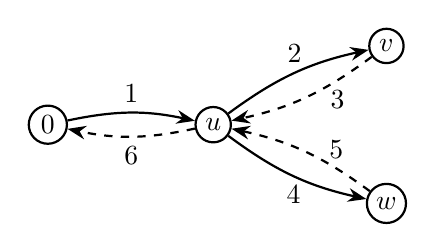
\begin{tikzpicture}[>=Stealth,thick,
  vertex/.style={circle,draw,inner sep=2pt},
  every edge/.style={font=\small}]
 \node[vertex] (o) at (0,0) {$0$};
 \node[vertex] (u) at (2.1,0) {$u$};
 \node[vertex] (v) at (4.3,1) {$v$};
 \node[vertex] (w) at (4.3,-1) {$w$};
 \draw[->] (o) to[bend left=12] node[above] {$1$} (u);
 \draw[->,dashed] (u) to[bend left=12] node[below] {$6$} (o);
 \draw[->] (u) to[bend left=12] node[above] {$2$} (v);
 \draw[->,dashed] (v) to[bend left=12] node[pos=.25,below] {$3$} (u);
 \draw[->] (u) to[bend right=12] node[below] {$4$} (w);
 \draw[->,dashed] (w) to[bend right=12] node[pos=.25,above] {$5$} (u);
\end{tikzpicture}
\caption{First visits (solid) and returns (dashed) in the walk
$0\to u\to v\to u\to w\to u\to0$.  Numbers give the chronological
step indices.  The three solid edges form the first-visit tree.
This diagram records only the walk topology.}
\label{fig:first-visit-tree}
\end{figure}

Recall that an occurrence $(i,p)$ is lit when
$p\mid n+b_{i-1}$.  Set
\begin{equation}\label{eq:fixed-line-labels}
 \mathcal F=\{p:\ p\text{ occurs on the line and either }
        p\in\mathcal C\text{ or }p\text{ occurs at least twice}\}.
\end{equation}
Write $n_{\mathcal F}$ for these residue coordinates.  We allow our
restrictions to depend on $n_{\mathcal F}$ and call the primes in
$\mathcal F$ the \emph{fixed labels}.  Here ``fixed'' refers to the
residues: the numerical line already specifies every prime value.
The set includes core primes occurring once on the line, but excludes
background core primes absent from it.  For a fixed tree prime $p$,
define its active vertices by
\[
 V_p=\{v\in V(\mathscr T):p\mid n+b(v)\}.
\]
The connected components of $V_p$ are those of the induced subgraph
on these vertices.  Adjacent active vertices force $p$ to divide
their edge label, since $p\nmid h$ for sufficiently large $B$.

A tree prime $p\notin\mathcal F$ is a center prime occurring on
exactly one step of the entire line.  Let $e_p$ denote its tree edge.
Call it \emph{corrupted} if a tree vertex other than the endpoints
of $e_p$ has an offset congruent to those endpoints modulo $p$.
This is a condition on the numerical line alone.

\begin{proposition}[Retained configurations]\label{prop:retained-lines}
For each closed line there is a predicate
$R_{\boldsymbol d}(n_{\mathcal F})\in\{0,1\}$ with the following
properties.  Whenever it equals one:
\begin{enumerate}
\item all core line occurrences are lit; no primitive specification
with support contained in $\mathcal F$ qualifies at a trace vertex;
and fewer than $t_0$ repeated center occurrences are unlit;
\item every fixed tree prime has $O(B^\rho)$ active components;
fewer than $B^{1-2\rho}$ fixed tree primes have more than one
active component;
\item fewer than $B^{1-2\rho}$ nonfixed tree primes are corrupted.
\end{enumerate}
The implicit constant is uniform in the line.  Moreover,
\begin{equation}\label{eq:retained-line-error}
 \sum_{\boldsymbol d}
  \E\left[|K_{\boldsymbol d}(n)|
       \prod_{j=0}^{\ell}\1_Y(n+b_j)
       (1-R_{\boldsymbol d}(n_{\mathcal F}))\right]
 \ll \exp(-B^{1+\eps/2}).
\end{equation}
The same exceptional estimates used in this proof remain valid
after adding the qualification indicators of at most $2t_0$
specifications and summing their recorded data, for the classes
discarded by an arithmetic saving.  Configurations excluded because
of a fixed forbidden specification instead vanish with the original
$Y$ factors.
\end{proposition}

We prove the proposition in three stages.  First we make active
sets connected on a small number of blocks.  Then a two-block
argument rules out many disconnected fixed labels.  Finally we
handle the accidental offset coincidences of singleton labels.

\subsection{Short gaps and connected blocks}

\begin{lemma}[Hitting paths in a forest]\label{lem:forest-path-hitting}
Let a finite forest carry a finite family of nonempty edge paths.
If the family has no $t$ pairwise edge-disjoint paths, some set of
fewer than $2t$ edges meets every path in the family.
\end{lemma}

\begin{proof}
Root each component.  The top of a path is its vertex nearest that
root.  Choose a path whose top has maximum depth, and mark its one
or two edges incident with the top.  Every path sharing an edge
with the chosen path must contain a marked edge.  Indeed, a path
sharing an edge below a mark and avoiding that mark remains wholly
in the component below it; its top would be strictly deeper.
Remove the paths hit by the marks and repeat.  The paths chosen at
successive stages are pairwise edge-disjoint.  There are fewer than
$t$ stages, so fewer than $2t$ marked edges suffice.
\end{proof}

\begin{lemma}[Connected activity on blocks]\label{lem:activity-blocks}
Except for configurations of zero contribution in
\eqref{eq:retained-line-error} or total absolute contribution
$O(\exp(-B^{1+\eps/2}))$, one can cut $O(t_0)$ edges of the
first-visit tree and cover the resulting forest by $O(B^\rho)$
connected blocks of diameter at most $L$.  The blocks cover every
remaining edge and every vertex of the original tree.  In each block,
the active set of every fixed tree prime is connected or empty.
Consequently each fixed tree prime has $O(B^\rho)$ whole-tree active
components.
\end{lemma}

\begin{proof}
An unlit core occurrence makes $K_{\boldsymbol d}=0$.  A primitive
specification supported on $\mathcal F$ and qualifying at a trace
vertex makes the corresponding $Y$ factor zero for every remaining
coordinate assignment.  Discard these configurations.  By
\Cref{lem:crude-count}, those with at least $t_0$ unlit repeated
center occurrences have the asserted negligible total.  Each of
these decisions uses only the line and $n_{\mathcal F}$.

Cut every tree edge having an unlit fixed occurrence.  There are
fewer than $t_0$ such edges.  In the remaining forest a \emph{gap
for $p$} is a path of length at most $L$ with active endpoints and
at least one interior vertex, all interior vertices being inactive,
for a fixed tree prime $p$.  Such a gap has no $p$-edge: an active
endpoint of a $p$-edge forces its
other endpoint to be active, while a $p$-edge with inactive
endpoints was cut.

Every gap contains a nonfixed prime label.  Otherwise all its
edge labels are fixed and lit, so the path is fully divisible.
Its nonzero total displacement is divisible by $p$, and its edges
avoid $p$.  Taking extra prime $p$ and the whole path as suffix
gives a qualifying specification.  By
\Cref{lem:primitive-descent}, a primitive one with fixed support
qualifies at a vertex of that tree path.  Every tree vertex is a
trace vertex, contrary to the preceding exclusion.

If there are $t_0$ edge-disjoint gaps, choose a nonfixed prime $q$
on each.  Each chosen prime occurs once on the full line, hence
nowhere on the other selected gaps.  The displacement of its gap
is linear in $q$ modulo the corresponding fixed prime $p$, with
coefficient $\pm h$ times the other prime factors of that edge.
This coefficient is invertible modulo $p$, since the gap is
$p$-free and $p\nmid h$.  The selected constraints do not involve
one another's variables.  Their paths and variables have the
description cost of \Cref{lem:triangular-saving}, which discards
this class.  The inequality $t_0\ge B^{2\eps}$ holds for large $B$.

Otherwise \Cref{lem:forest-path-hitting} supplies fewer than
$2t_0$ further cuts meeting every gap.  For each remaining piece
traverse every edge twice and split that traversal into segments
of at most $L$ steps.  The edges and vertices in a segment form
a connected subtree of diameter at most $L$; include a singleton
block for a piece with no edges.  There are
\[
 O(\ell/L+t_0+1)=O(B^\rho)
\]
blocks.  They may overlap.  Any two active vertices in a block
have their joining path inside that block.  An inactive portion
on it would give a surviving short gap, impossible after the cuts.
Thus activity is connected or empty on each block.  Each block
meets at most one whole-tree active component, and every such
component has a vertex in a block.  This proves the component bound.
\end{proof}

\subsection{Comparing two blocks}

The active sets are now connected within each block.  To compare
different components for a fixed prime $p$, suppose blocks $1$ and
$2$ meet those components.  Choose a root $c_j$ in block $j$ and an
active representative $x_p^j$ there.  Since the representatives have
distinct integer offsets,
\begin{equation}\label{eq:two-block-constraint}
 p\mid K+\bigl(b(x_p^2)-b(c_2)\bigr)
           -\bigl(b(x_p^1)-b(c_1)\bigr)\ne0,
 \qquad K=b(c_2)-b(c_1).
\end{equation}
To apply the divisibility case of \Cref{lem:triangular-saving}, we
seek roots and representatives for which both local paths contain
no edge label divisible by $p$.  For many selected primes at once,
we also need a common order in which every selected prime appearing
on either path comes earlier than $p$.  Once $K$ is specified separately, these
conditions give the required triangular dependence.  The next lemma
supplies the choices.

\begin{lemma}[Rerooting two blocks]\label{lem:reroot-constraints}
Let two connected blocks of a tree and $m$ distinct prime indices
$p$ be given.  For each index let $V_p$ be a vertex subset, and let
$A_p^j$ be its intersection with block $j$.  Suppose these
intersections are nonempty and connected.  Edges have labels
containing at most $J$ prime factors.  In either block, an edge has
both endpoints in $A_p^j$ if and only if its label contains $p$.
Assume also that $A_p^1$ and $A_p^2$ lie in distinct components of
the subgraph induced by $V_p$ in the whole tree.

There are roots $c_j$ in block $j$, a set of
$\gg m^{1/8}/(2J+1)$ retained indices, and an order on those indices
with the following property.  If $x_p^j$ is the nearest vertex of
$A_p^j$ to $c_j$, both paths from $c_j$ to $x_p^j$ avoid $p$, and
any retained prime label on either path occurs earlier in the order.
The two representatives $x_p^1,x_p^2$ are distinct.
\end{lemma}

\begin{proof}
Start with arbitrary roots.  A connected vertex set in a tree
contains the entire path between any two of its vertices.  It
therefore has a unique nearest vertex to a chosen root.  The
root-to-$x_p^j$ path avoids $p$-edges.  If a retained label $q$
occurs on this path, both ends of its edge lie in $A_q^j$;
the nearest vertex $x_q^j$ is then a strict ancestor of $x_p^j$.
Thus dependencies are contained in the two strict ancestor orders.
Indices with equal nearest points are incomparable.

Every finite partially ordered set with $u$ elements has a chain
or an antichain of size at least $\sqrt u$: partition its elements
by the length of a longest chain ending there.  Apply this to the
first ancestor order.  If an antichain is obtained, there are no
dependencies from block 1 among its indices, so depth order in
block 2 suffices.  Otherwise apply the same argument in block 2
on the selected chain.  An antichain there similarly suffices.
In the remaining case we have chains in both blocks with at least
$m^{1/4}$ indices.  The Erd\H{o}s--Szekeres monotone-subsequence theorem
\cite[p.~467]{ErdosSzekeres1935} shows that two total orders have a
common agreeing or reversed subsequence of size at least the square
root of their length.  To recall the elementary argument, assign to each position the lengths
of the longest increasing and decreasing subsequences ending
there.  Two positions have different pairs, so if both lengths
are less than $\sqrt u$ there cannot be $u$ positions.  We thus
retain at least a constant times $m^{1/8}$ indices.  Agreeing
orders already give the conclusion.

Suppose the orders are reversed.  In block 2 take the segment
from its root to the farthest selected $x_p^2$.  The intersection
of each $A_p^2$ with that segment is a closed vertex interval
beginning at $x_p^2$; these left endpoints are distinct.  At a
vertex of the segment, each positive-length interval containing
it contains an incident segment edge.  Each of the at most two
such edges has at most $J$ prime factors.  At most one interval
can consist of that vertex alone.  Hence at most $2J+1$ intervals
overlap at a vertex.  Greedily coloring closed intervals in order
of their left endpoints uses at most $2J+1$ colors: an existing
color is available only if its preceding right endpoint is
strictly earlier than the new left endpoint.  One color retains
at least a $1/(2J+1)$ fraction of pairwise vertex-disjoint intervals.

Reroot block 2 at the far end of the segment.  The nearest point
of $A_p^2$ is now the right endpoint of its interval.  Indeed, for
any vertex of $A_p^2$ off the segment, its projection onto the
segment lies in that interval, because the path from $x_p^2$ to
the vertex lies in $A_p^2$.  The path from the new root first
reaches $A_p^2$ at the right endpoint.  This also proves that
off-segment branches cannot change the nearest point.

The right endpoints of vertex-disjoint intervals have the same
order as their left endpoints along the original segment.  Seen
from its other end, that order reverses.  The two block orders
therefore agree after rerooting.  The first paragraph applies to
the new root as well and proves the dependency assertion.  Each
representative stayed in the same whole-tree component for its
prime, so the two representatives for that prime are still distinct.
\end{proof}

\begin{lemma}[Few disconnected fixed labels]\label{lem:few-disconnected}
Among the configurations retained by \Cref{lem:activity-blocks},
those with at least $B^{1-2\rho}$ fixed tree primes having multiple
active components have total absolute contribution
$O(\exp(-B^{1+\eps/2}))$.
\end{lemma}

\begin{proof}
For every such prime choose two blocks meeting distinct whole-tree
active components.  There are $O(B^{2\rho})$ ordered block pairs,
so one pair serves $m\gg B^{1-4\rho}$ primes.  Inside each block,
the active set is nonempty and connected.  Every edge carrying a
fixed prime has active endpoints after the earlier cuts, and the
converse follows from $p\nmid h$.  Apply
\Cref{lem:reroot-constraints} and then specify the common integer
\[
 K=b(c_2)-b(c_1),\qquad |K|=O(\ell H).
\]
Each retained prime gives the test \eqref{eq:two-block-constraint}.
The expression is independent of $p$, since both local paths
avoid it.  It involves only earlier retained variables by the
lemma.  Its nonvanishing follows from distinctness of the two
representatives and the distinct integer offsets of tree vertices.
The number of tests is
\[
 \gg \frac{B^{(1-4\rho)/8}}{J}
   =\frac{B^{1/10}}{O(\log B)}>B^{2\eps}
\]
for large $B$.

Roots, endpoints, and prime choices can be recorded with the
entropy allowed in \Cref{lem:triangular-saving}.  Choose $K$ only
after the rerooting; its $O(\ell H+1)$ possibilities cost
$\exp(O(B))$.  Although its original value depends on the labels,
fixing it and dropping that defining equation enlarges a positive
sum.  The local path expressions then have the required triangular
dependence.  Retain their nonzero tests under this enlargement and
apply \Cref{lem:triangular-saving}.
\end{proof}

\subsection{Accidental coincidences of singleton labels}

The preceding argument concerned fixed residue coordinates.  A
nonfixed tree prime requires a different test: its residue must
remain free, so we use only numerical coincidences between offsets.

\begin{lemma}[Few corrupted singleton labels]\label{lem:few-corrupted}
Lines having at least $B^{1-2\rho}$ corrupted nonfixed tree primes
have total absolute contribution
$O(\exp(-B^{1+\eps/2}))$.
\end{lemma}

\begin{proof}
For every corrupted prime choose a witnessing vertex outside its
edge endpoints, and put $D=\lfloor B^{1-3\rho}\rfloor$.  Distance
from a vertex to an edge means its minimum tree distance to the two
endpoints.  Suppose first that at least half the selected witnesses have distance at
most $D$ from their prime edge.  Use the path from the nearer edge
endpoint to its witness.  This path avoids the prime's sole edge,
so its nonzero displacement is independent of that prime and is
divisible by it.  The expression contains at most $JD$ other
prime labels.

On the selected primes draw a directed dependency edge $p\to q$
if the test for $p$ contains $q$.  Its outdegree is at most $JD$.
Every induced subgraph of the underlying undirected graph has
average degree at most $2JD$.  Successively choose a vertex of
degree at most $2JD$ and delete its neighbors.  The resulting
independent set has size at least a constant times
\[
 \frac{B^{1-2\rho}}{JD+1}\gg\frac{B^\rho}{J}>B^{2\eps}.
\]
Its tests have no selected-variable dependencies.  They are
covered by \Cref{lem:triangular-saving}.

Otherwise at least half the witnesses have distance greater than
$D$.  Cover the full tree by $O(\ell/D+1)=O(B^{3\rho})$ connected
traversal blocks of diameter at most $D$, as in the earlier
construction.  Assign each prime edge to a block containing that
edge and its witness to a block containing that vertex.  One
ordered pair serves $\gg B^{1-8\rho}$ primes.  No selected prime
edge has an endpoint in the second block: its corresponding
witness lies there, so that would put it at distance at most $D$.
Consequently paths inside the second block contain no selected
prime label.

Root the two blocks at $c_1,c_2$.  In block 1 let $x_p^1$ be the
nearer endpoint of the prime edge; in block 2 let $x_p^2$ be its
witness.  The first local path avoids $p$.  If it contains a
selected prime $q$, the nearer endpoint of the $q$-edge is a
strict ancestor of $x_p^1$.  Thus the tests
\eqref{eq:two-block-constraint}, after specifying the common root
offset, are triangular in the depths of the first-block
endpoints.  The second local paths introduce no selected
variables.  Each tested displacement is nonzero because its
witness differs from the chosen edge endpoint.  Since
$1-8\rho=3/5>2\eps$, there are more than enough tests for
\Cref{lem:triangular-saving}.  All choices of witnesses, blocks,
roots, and paths fit its description bound.
\end{proof}

\begin{proof}[Proof of \Cref{prop:retained-lines}]
Define $R_{\boldsymbol d}$ by retaining the conditions obtained
in \Cref{lem:activity-blocks,lem:few-disconnected,lem:few-corrupted}.
Every activity and occurrence status of a fixed label is determined
by $n_{\mathcal F}$; fixed forbidden qualifications use only those
coordinates; corruption uses only numerical offsets.  Covers and
witnesses can be chosen by fixed finite ordering whenever they
exist.  Thus $R_{\boldsymbol d}$ depends on no free center residue.

The zero exclusions vanish with $K_{\boldsymbol d}\prod_j\1_Y$.
The other excluded classes have the stated absolute contribution
by the three lemmas, yielding \eqref{eq:retained-line-error}.
Their proofs used precisely the majorants of
\Cref{lem:crude-count,lem:triangular-saving}, which allow up to
$2t_0$ attached specifications.  Their retained tests depend only
on the numerical line and fixed residues, and are unchanged when
qualification indicators are added.  This proves the additional assertion as well.
\end{proof}

We may therefore impose the retained predicate before estimating
the remaining conditional averages.  This preserves the residue
coordinates of singleton center labels.  The next section deals
with the remaining dependence of the factors $\1_Y$ on those
coordinates by expanding them into short lists of qualification
conditions.

\section{A conditional cylinder sieve}\label{sec:cylinder-sieve}

The restrictions $n+b_j\in Y$ still involve the residue coordinates
outside the fixed set $\mathcal F$.  We replace their product by a sum
of conditions from short lists of primitive specifications.  In each
term the remaining coordinates are averaged before taking an absolute
value; this preserves the cancellation needed in the trace estimate.
The error will contain many specifications with distinct private prime
coordinates, which supply enough arithmetic constraints to apply
\Cref{lem:triangular-saving}.

The intersection rank and the extraction of constraints from its
witnesses adapt Pilatte's construction
\cite[Definition~13.3 and Lemmas~13.4 and~13.6]{Pilatte26}.
The associated truncation belongs to the composite-modulus sieve
developed in \cite[Section~3]{HR21} and
\cite[Appendix~B]{Pilatte26}.  We prove the finite-cylinder statement
and its application here, including the effect of conditioning.

\subsection{Truncating an intersection poset}

Let $\Omega=\prod_{p\in P}\Omega_p$ be a finite product, with
$|\Omega_p|\ge2$ for every $p$.  An \emph{exact cylinder} specifies one
value at each coordinate in a subset of $P$ and imposes no condition at
the other coordinates.  Its \emph{support} is the set of specified
coordinates, and its \emph{width} is the size of that support.

Let $\mathscr E$ be a finite family of proper, nonempty exact cylinders.
Identify duplicate cylinders.  Let $\mathscr P$ consist of the nonempty
intersections of subfamilies of $\mathscr E$, including the empty-family
intersection $\widehat0=\Omega$.  Order $\mathscr P$ by reverse inclusion:
$I\le J$ means $I\supseteq J$.  For $I\in\mathscr P$, define
\begin{equation}\label{eq:cylinder-rank}
 \operatorname{rk}(I)=
 \max\left\{|\mathscr A|:\begin{array}{l}
   \mathscr A\subseteq\{E\in\mathscr E:I\subseteq E\},\\
   \text{each }E\in\mathscr A\text{ has a support coordinate}\\
   \text{absent from every other member of }\mathscr A
 \end{array}\right\}.
\end{equation}
The empty family is allowed in this maximum.  A coordinate as in
\eqref{eq:cylinder-rank} is called \emph{private} to its member of
$\mathscr A$.  All events in such a family have compatible prescribed
values because they contain the nonempty intersection $I$.

Write $\mu(\widehat0,I)$ for the M\"obius coefficients of this finite
poset, characterized by
\[
 \sum_{I\le J}\mu(\widehat0,I)=\1_{J=\widehat0}.
\]
Their role is inclusion--exclusion with equal intersections collected
into one term.  This is M\"obius inversion in the incidence algebra of a
finite poset; see \cite[Section~3]{Rota1964}.  The chain expansion used
below is the one in \cite[Section~3, Proposition~6]{Rota1964}.

\begin{lemma}[Finite-cylinder truncation]\label{lem:cylinder-truncation}
Suppose that the cylinders in $\mathscr E$ have width at most $w\ge1$.
For an integer $t\ge1$, put $M=tw$, and let
\[
 \mathscr H_t=\{J\in\mathscr P:\operatorname{rk}(J)\ge t,
       \ J\text{ is generated by at most }t\text{ members of }\mathscr E\}.
\]
Then the rank is nondecreasing on $\mathscr P$, every $I\in\mathscr P$
is generated by at most $\operatorname{rk}(I)$ events, and
\begin{equation}\label{eq:cylinder-width}
 |\operatorname{supp}(I)|\le w\operatorname{rk}(I).
\end{equation}
For every $x\in\Omega$,
\begin{equation}\label{eq:cylinder-truncation}
 \left|\1_{x\notin\bigcup_{E\in\mathscr E}E}
       -\sum_{\operatorname{rk}(I)<t}\mu(\widehat0,I)\1_I(x)\right|
 \le 2^M\max(1,M^{M+1})\sum_{J\in\mathscr H_t}\1_J(x).
\end{equation}
Every coefficient retained in the sum on the left has absolute value
at most $\max(1,M^{M+1})$.  Every intersection on the right has width
at most $M$, even if its rank is greater than $t$.
\end{lemma}

\begin{proof}
If $I\le J$, every event containing $I$ also contains $J$.  Thus every
family admitted for the maximum defining $\operatorname{rk}(I)$ is
admitted for $\operatorname{rk}(J)$, proving monotonicity.
Choose an inclusion-minimal family generating $I$.  Each member must
have a private coordinate: otherwise all its prescribed values already
follow from the other members, since the prescriptions are compatible,
and it can be removed.  Its size is therefore at most
$\operatorname{rk}(I)$, proving \eqref{eq:cylinder-width} as well.

Fix $J\in\mathscr P$ and let $m=|\operatorname{supp}(J)|$.  An element
of the interval $[\widehat0,J]$ is determined by its support: its values
must be the corresponding restrictions of those prescribed by $J$.
Consequently this interval has at most $2^m$ elements.  Along a strict
chain from $\widehat0$ to $J$, supports grow strictly, so there are at
most $m$ steps.  A chain of $k$ steps is specified by recording, for
each coordinate of $\operatorname{supp}(J)$, the step at which it
enters.  There are at most $k^m$ such chains.  Expanding the inverse of
the poset's upper triangular incidence matrix, or applying the M\"obius
recursion repeatedly, gives the alternating sum over these chains.
Thus, for $m\ge1$,
\begin{equation}\label{eq:cylinder-mobius}
 |\mu(\widehat0,J)|\le\sum_{k=1}^m k^m\le m^{m+1};
\end{equation}
the coefficient at $\widehat0$ is $1$.  This proves the asserted
coefficient bound for intersections of rank below $t$.

For $x\in\Omega$, let $J_x$ be the intersection of all events satisfied
at $x$, with $J_x=\widehat0$ if none are satisfied.  An intersection
$I\in\mathscr P$ contains $x$ if and only if $I\le J_x$.  Indeed any
family generating $I$ then consists of events satisfied at $x$.
It follows that
\begin{equation}\label{eq:cylinder-full-sum}
 \sum_{I\in\mathscr P}\mu(\widehat0,I)\1_I(x)
    =\sum_{I\le J_x}\mu(\widehat0,I)
    =\1_{J_x=\widehat0}.
\end{equation}
Since no forbidden event is the whole space, the last expression is
precisely the avoidance indicator in \eqref{eq:cylinder-truncation}.

If $\operatorname{rk}(J_x)<t$, monotonicity shows that the truncated
sum contains the entire interval $[\widehat0,J_x]$, so it is exact.
Suppose instead that $\operatorname{rk}(J_x)\ge t$.  Given any
$I\le J_x$ of rank below $t$, successively intersect it with events
satisfied at $x$ until reaching $J_x$.  Let $K$ be the first intersection
whose rank is at least $t$, and let $K^-$ be its immediate predecessor.
Replace the generating family for $K^-$ by an inclusion-minimal one.
It has at most $t-1$ members.  Adjoining the event that produces $K$
shows that $K$ is generated by at most $t$ events.  Thus
\[
       I\le K\le J_x,\qquad K\in\mathscr H_t,
       \qquad |\operatorname{supp}(K)|\le M.
\]
This argument allows the rank to jump by more than one.  The
re-minimization of the predecessor, rather than the length of the
successive list, bounds the number of generators.

Every satisfied low-rank $I$ is therefore below a satisfied member of
$\mathscr H_t$.  For any one such member there are at most $2^M$
possible predecessors $I$, by the interval bound already proved.
The exact avoidance indicator is zero in the present case.  Bounding
each retained coefficient by \eqref{eq:cylinder-mobius} now gives
\eqref{eq:cylinder-truncation}.
\end{proof}

\subsection{Applying the truncation after conditioning}

Return to a fixed numerical line $\boldsymbol d$.  Its fixed prime set
$\mathcal F$ consists of its core labels and its repeated labels, as in
\Cref{sec:thinning}.  In particular, core primes absent from the line
are not added to $\mathcal F$.  Write
$R_{\boldsymbol d}(n_{\mathcal F})$ for the indicator of the conditions
retained in \Cref{prop:retained-lines}.

Condition on $n_{\mathcal F}$ with $R_{\boldsymbol d}=1$.  At every
$n+b_j$, take the primitive forbidden specifications compatible with
these fixed residues.  Omit their fixed-coordinate tests, leaving
exact cylinders on the coordinates $\mathcal S\setminus\mathcal F$.
Each has width at most $LJ+1$.  There is no whole-space event: such an
event would be a qualifying primitive specification using only fixed
primes, excluded by the retained conditions.  Avoiding these residual
events is exactly the condition $n+b_j\in Y$ for every $j$.

For a list $\mathfrak L$ of primitive specifications attached at line
indices $0,\ldots,\ell$, let $I_{\mathfrak L}(n)$ be the indicator that
all its specifications qualify, including their fixed-coordinate
tests.  The empty list has indicator $1$.  Let
$\mathscr L_{<t_0}(\boldsymbol d)$ denote all ordered such lists of length
less than $t_0$.  These are finite families at the fixed graph
parameters.  We will use the bound
\begin{equation}\label{eq:cylinder-budget}
 M_0=t_0(LJ+1)=O(B^{1-\rho+4\eps}\log B),\qquad
 M_0\log B=o(B).
\end{equation}
In particular, the coefficient and error factors in
\Cref{lem:cylinder-truncation} are $\exp(O(M_0\log B))$.

A low-rank intersection is generated by fewer than $t_0$ residual
events.  Choose one realizing primitive specification for each event.
The conjunction of their full qualification indicators equals the
intersection indicator at the conditioned residues.  Different
intersections cannot have the same chosen generating list, since that
list determines its intersection.  We may therefore bound their sum
by the sum over $\mathscr L_{<t_0}(\boldsymbol d)$ without a multiplicity
loss.

For an intersection in $\mathscr H_{t_0}$, choose at most $t_0$
generating events and exactly $t_0$ events witnessing its rank.  The
latter may be selected from a larger irredundant family; deleting other
members preserves their private coordinates.  The witnessing events
contain the intersection.  Consequently adjoining them to the
generating list leaves its indicator unchanged.  After choosing
realizing primitive specifications, each witness has a prime outside
$\mathcal F$ that occurs in none of the other witness specifications.
These choices may depend on $n_{\mathcal F}$, which is harmless:
the preceding assertions and the uniform coefficient bounds apply
pointwise at each fixed-coordinate assignment.

We have thus reduced the truncation error to jointly qualifying lists
of at most $2t_0$ specifications, including $t_0$ witnesses with private
primes outside $\mathcal F$.  The next lemma shows that these error
lists impose many triangular constraints on their numerical prime
labels.

\begin{lemma}[Constraints from private primes]\label{lem:cylinder-witnesses}
Let $\boldsymbol d$ be a numerical closed line, and let $\mathcal F$ contain
its core prime labels and all labels occurring at least twice on the
line.  Suppose $t_0$ primitive specifications attached at line vertices
qualify simultaneously.  Suppose that each has a prime outside
$\mathcal F$ absent from every other specification in this family.
For sufficiently large $B$, their numerical labels satisfy a triangular
system on at least $B^{2\eps}$ distinct selected prime variables of the
kind in \Cref{lem:triangular-saving}.  Each constraint uses one intrinsic
suffix displacement, or the difference of two witness prefixes and a
line segment.  Its nonzero expressions have logarithmic size
$O(B\log B)$ even when numerical label-size restrictions are dropped.
\end{lemma}

\begin{proof}
Order the witnesses by nondecreasing attachment indices
$k_1,\ldots,k_{t_0}$; break ties arbitrarily.  For witness $j$, choose a
private prime $q_j\notin\mathcal F$, write $p_j$ for its extra prime,
and choose a tail prime $r_j$ as in
\Cref{lem:primitive-properties}.  Thus $r_j$ occurs only in its final
constant block.  That lemma supplies two coefficient facts:
\begin{enumerate}[label=(\roman*)]
\item the intrinsic suffix displacement divisible by $p_j$ is linear
in a tail-only prime, with coefficient nonzero modulo $p_j$;
\item if a prime occurs before the constant tail, its coefficient in
the prefix displacement immediately preceding that tail is nonzero
modulo $r_j$.
\end{enumerate}
All private primes $q_j$ are distinct.  Each occurs at most once as a
label on the original line, because it is outside $\mathcal F$.
We divide into three cases to control every dependence on another
selected variable.

\paragraph{Private primes in intrinsic suffix constraints.}
Suppose at least $t_0/10$ witnesses have $q_j=p_j$ or have $q_j$
occurring only in the constant tail.  In the first situation $q_j$
divides the intrinsic suffix displacement, which is nonzero by
simplicity and does not involve $q_j$.  In the second situation use
that suffix constraint as a linear congruence in $q_j$ modulo $p_j$;
its coefficient is nonzero by (i).  The private-prime property excludes
every other selected $q$ from the witness, including from its modulus.
These constraints have no dependencies on the other selected
variables and hence form a triangular system.

\paragraph{Tail primes first or last appearing among the witnesses.}
Suppose at least $t_0/10$ witnesses have $r_j$ absent from every earlier
witness.  Select these tail primes in increasing witness order.  They
are distinct: equality between two would make the latter prime occur
in an earlier witness.  Use the intrinsic suffix congruence for each
selected $r_j$.  No later selected tail prime occurs in this witness,
by its defining absence property.  This also excludes later selected
variables from the modulus $p_j$.  Thus each constraint uses only its
own variable, earlier selected variables, and nonselected variables,
and its coefficient is nonzero modulo $p_j$ by (i).
If instead at least $t_0/10$ witnesses have $r_j$ absent from every later
witness, the same argument in decreasing witness order applies.

\paragraph{Comparing two activities of a shared tail prime.}
If none of these cases applies, fewer than $3t_0/10$ witnesses have
been excluded by their three respective conditions.  Retain at least
$t_0/2$ witnesses for which $q_j$ occurs before the tail and $r_j$
appears in both an earlier and a later witness.  Since $q_j$ occurs
at most once on the original line, it is absent either from all steps
$1,\ldots,k_j$ or from all steps $k_j+1,\ldots,\ell$.  At least
$t_0/4$ of the retained witnesses satisfy the same one of these two
absence conditions.

First consider the family absent from steps $1,\ldots,k_j$, ordered
increasingly by attachment index.  For its witness $j$, choose an
earlier witness $i=i(j)$ using $r_j$.  In witness $i$, choose a vertex
at which $r_j$ is active: its starting vertex if $r_j$ is its extra
prime, or the origin of an edge carrying $r_j$ otherwise.  Let $T_i$
be this vertex's offset relative to that witness's start.  Let $P_j$
be the prefix displacement of witness $j$ immediately preceding its
constant tail.  Joint qualification implies
\begin{equation}\label{eq:cylinder-comparison}
 b_{k_j}-b_{k_i}+P_j-T_i\equiv0\pmod{r_j}.
\end{equation}
The coefficient of $q_j$ in this congruence is exactly its coefficient
in $P_j$: privateness excludes it from witness $i$, and the selected
absence condition excludes it from the line segment between
$k_i$ and $k_j$.  This coefficient is nonzero modulo $r_j$ by (ii).

Now take a later selected private variable $q_s$.  It occurs in
neither witness $i$ nor witness $j$, by privateness.  Moreover
$k_s\ge k_j$, and its own absence condition excludes it from every
line step through $k_s$, hence from the segment in
\eqref{eq:cylinder-comparison}.  Thus no later selected variable occurs
in that congruence.  The modulus $r_j$ is not any selected private
prime: it differs from $q_j$ because $q_j$ occurs before the tail,
and it differs from all other $q_s$ by privateness.  This proves
triangularity in increasing order.  Equal attachment indices merely
make the corresponding line segment empty.

For the family absent from steps after $k_j$, order the witnesses
decreasingly and compare witness $j$ to a later witness containing
$r_j$.  Equation \eqref{eq:cylinder-comparison} has the same form, now
with its line segment after $k_j$.  A later selected variable in this
decreasing order has attachment $k_s\le k_j$ and is absent from all
steps after $k_s$, so it is absent from that segment.  Privateness
excludes it from the two witness prefixes.  Fact (ii) again supplies
the nonzero coefficient.  This gives a triangular system in decreasing
order.  The attained comparison displacement may equal zero; that
causes no difficulty, since we use an invertible linear congruence,
not a divisibility constraint with the selected prime as modulus.

Every case provides at least $t_0/20$ selected variables for sufficiently
large $B$, allowing for integer parts.  This is greater than
$B^{2\eps}$.  Each label is a squarefree product of at most $J$ primes
at most $e^B$, so its logarithm is at most $BJ=O(B\log B)$ even without
the divisor-bin restrictions.  A suffix or a comparison above uses
$O(\ell+L)$ such terms.  Every nonzero expression consequently has
logarithmic size $O(B\log B)$.  The constraint choices are specified
by witness and line positions and prime slots, within the enumeration
allowed in \Cref{lem:triangular-saving}.  All its hypotheses are now
verified.
\end{proof}

\begin{proposition}[Reduction to short qualification lists]
\label{prop:cylinder-reduction}
For the retained line and fixed-coordinate data of
\Cref{prop:retained-lines}, there is a factor
$\mathfrak C_B=\exp(O(M_0\log B))$ such that
\begin{align}
 &\sum_{\boldsymbol d}\E_{\mathcal F}
   \left[R_{\boldsymbol d}
     \left|\E_{\mathcal S\setminus\mathcal F}
          K_{\boldsymbol d}(n)\prod_{j=0}^{\ell}\1_Y(n+b_j)\right|\right]
       \notag\\
 &\quad\le \mathfrak C_B\sum_{\boldsymbol d}\E_{\mathcal F}
   \left[R_{\boldsymbol d}
     \sum_{\mathfrak L\in\mathscr L_{<t_0}(\boldsymbol d)}
       \left|\E_{\mathcal S\setminus\mathcal F}
                      K_{\boldsymbol d}(n)I_{\mathfrak L}(n)\right|\right]
       +O\!\left(e^{-B^{1+\eps/2}}\right).
       \label{eq:cylinder-reduction}
\end{align}
Here each sum runs over numerical closed lines, $\mathcal F$ is the
fixed prime set of that line, and every list indicator imposes full
qualification of its specifications.
\end{proposition}

\begin{proof}
At fixed $\boldsymbol d,n_{\mathcal F}$ with $R_{\boldsymbol d}=1$, apply
\Cref{lem:cylinder-truncation} to the residual cylinders with
$t=t_0$ and $w=LJ+1$.  Multiply the identity with its pointwise error
bound by $K_{\boldsymbol d}$ and integrate the residual coordinates.
For the low-rank sum, take the absolute value after each such integral
and use the generating lists already constructed.  The coefficient
bound gives the main term on the right of
\eqref{eq:cylinder-reduction}.

For the error, take the absolute value of $K_{\boldsymbol d}$ inside the
integral and use the generating and witnessing lists described above.
After integrating the fixed coordinates, their indicators require
joint qualification of at most $2t_0$ specifications, including the
$t_0$ witnesses with private primes outside $\mathcal F$.
We may drop the retained-data restriction in this positive bound.
\Cref{lem:cylinder-witnesses} supplies at least $B^{2\eps}$ triangular
constraints for each nonzero contribution.

Refine the error count by the lit or unlit status of every line
occurrence.  Joint qualification fixes one residue for each distinct
prime used by the specifications, or is inconsistent and contributes
zero.  For each refinement, \Cref{lem:crude-count} gives
$A^{\ell J}\prod_p p^{-1}$, with the product over distinct prime labels,
rather than charging a shared residue repeatedly.  The line and lists
have at most
\[
       \ell J+2t_0(LJ+1)=O(B\log B)
\]
prime slots.  Their equality patterns, occurrence statuses and all
choices of witness constraints have cost $\exp(O(B\log^2 B))$.
These are exactly the
positive majorant and description budget required by
\Cref{lem:triangular-saving}.  Its reverse elimination applies to the
system just supplied by \Cref{lem:cylinder-witnesses} and gives
$O(e^{-B^{1+\eps/2}})$.
The additional factor $\mathfrak C_B$ is absorbed by the same estimate, since
\eqref{eq:cylinder-budget} gives $\log \mathfrak C_B=o(B)$ whereas the saving
before this final simplification is $\exp(-\Omega(B^{1+\eps}))$.
This proves the proposition.
\end{proof}

The reduction has preserved a signed average at the unfixed coordinates.
For its use in the next section, it is useful to distinguish
$\mathcal C'=\mathcal C\setminus\mathcal F$ and
$\mathcal Z'=\mathcal Z\setminus\mathcal F$.  For each list,
\begin{equation}\label{eq:cylinder-core-order}
 \left|\E_{\mathcal S\setminus\mathcal F}
              K_{\boldsymbol d}I_{\mathfrak L}\right|
 \le \E_{\mathcal C'}
       \left|\E_{\mathcal Z'}K_{\boldsymbol d}I_{\mathfrak L}\right|.
\end{equation}
This is only Fubini's theorem and the triangle inequality.  In the
inner average all core coordinates are held fixed, so the cutoffs are
fixed there; the free center coordinates still retain their signs.
The core coordinates can subsequently be integrated against positive
bounds.  In particular, \eqref{eq:cylinder-core-order} does not enlarge
$\mathcal F$ or change the private-coordinate rank used in the sieve.

\section{Summing the trace}\label{sec:trace-count}

We now prove the high-trace estimate.  The input from
\Cref{prop:retained-lines} is a description of the activities of the fixed
primes on the first-visit tree.  The input from
\Cref{prop:cylinder-reduction} replaces vertex deletion by short lists of
qualifying primitive specifications.  The remaining task is to sum the
resulting conditional averages without losing a constant for every prime
occurrence.  An exact identity for weighted subtrees makes this possible.

We retain the notation $\mathscr T$, $b(v)$ and $r_*$ for the first-visit
tree, its integer offsets and the number of returns.  In this section a
subtree is a connected subgraph of $\mathscr T$; its \emph{top} is its
vertex nearest the root.  Put
\[
 s(v)=\#\{\text{children of }v\},\qquad
 M_0=t_0(LJ+1),\qquad N_{\mathrm{exc}}=B^{1-\rho/2}.
\]
We call a tree edge $u\longrightarrow v$ \emph{good} if
$s(u)=s(v)=1$, $u$ is not the root, and neither endpoint belongs to any
return step.  Write $\mathcal G$ for the set of good edges.  These
conditions ensure that an uncorrupted prime occurring just on such an
edge has exactly two normalization factors on its lit residue.

For all but a small exceptional set of good edges, we will obtain the
factor $B^{-1+\eta}$ from a core-prime restriction to the divisor interval,
or a stronger penalty from a core cutoff.  Returns receive a cutoff
penalty as well.  Signed center-prime averages provide the further saving
needed in the high-trace estimate.  The weighted-subtree identity below
will let us sum the prime labels without losing these gains.

\subsection{Tree geometry and weighted subtrees}

\begin{lemma}\label{lem:trace-topology}
For a closed line of length $\ell$ with $r_*$ returns, the topology of first
visits and returns, together with all step signs, has at most
$4^\ell(\ell+1)^{r_*}$ possibilities.  Its tree satisfies
\begin{equation}\label{eq:trace-bad-edges}
 |E(\mathscr T)\setminus\mathcal G|\le 10(r_*+1),\qquad
 \ell=|E(\mathscr T)|+r_*.
\end{equation}
Once the labels of the tree edges and this topology are specified, every
return label is determined.
\end{lemma}

\begin{proof}
At each step record whether its destination is new and record its sign.
At each return record one of at most $\ell+1$ previously visited vertices.
These data give the stated bound.  A tree-edge label and its sign specify
the difference of its endpoint offsets; all offsets are consequently
determined, and a return label must be the absolute endpoint difference
divided by $h$.  We retain only assignments for which the abstract vertices
have distinct offsets and all these return labels belong to $\mathcal D$.
There is no independent choice of a return label.

Let $q$ be the number of leaves and $b$ the number of vertices with at
least two children.  The adding steps occur in at most $r_*+1$ runs,
each a downward path, so $q\le r_*+1$.  Also $b\le q-1$ and
\[
 \sum_{s(v)\ge2}s(v)=q+b-1.
\]
The number of edges incident with a leaf or such a branch vertex is
therefore at most $4q$.  There are at most $2r_*$ endpoints of return
steps.  An endpoint that has not already been counted is unary and is
incident with at most two tree edges, giving at most $4r_*$ further
edges.  The root adds at most one edge unless it was already counted as a
branch vertex.  These bounds imply \eqref{eq:trace-bad-edges}.
\end{proof}

For $a\in\{C,Z\}$ and a subtree $Q$ with at least one edge define
\begin{equation}\label{eq:subtree-weights}
 u_a(Q)=A_a^{|E(Q)|}\prod_{v\in V(Q)}\beta_a^{s(v)},\qquad
 S_a(\mathscr T)=\sum_{v\in V(\mathscr T)}(1-\beta_a^{s(v)}).
\end{equation}
The degrees in this definition are those of the full tree.

\begin{lemma}\label{lem:subtree-weight}
For every finite rooted tree and every $A_a>0$ with
$\beta_a=(1+A_a)^{-1}$,
\begin{equation}\label{eq:subtree-identity}
 \sum_{Q:\,|E(Q)|\ge1}u_a(Q)=S_a(\mathscr T)\le |V(\mathscr T)|.
\end{equation}
\end{lemma}

\begin{proof}
Start at a prescribed vertex $v$.  At every reached vertex include each
child edge independently with probability $A_a\beta_a$ and exclude it
with probability $\beta_a$.  The resulting connected subtree has top
$v$.  A particular outcome $Q$ has probability
\[
 (A_a\beta_a)^{|E(Q)|}
 \beta_a^{\sum_{w\in V(Q)}s(w)-|E(Q)|}=u_a(Q).
\]
The outcome with no edges has probability $\beta_a^{s(v)}$.
Sum the other probabilities, then sum over the possible tops $v$.
\end{proof}

The exact sum in \eqref{eq:subtree-identity} will cancel the background
exponential in the primewise estimate below.  To retain the additional
center-prime saving, we also use modified weights.  These anticipate the
primewise bounds proved in \Cref{lem:trace-integration}: the reduction on
a single good edge comes from a signed average, while the increase on
other single edges permits an absolute bound.
Set $\widetilde u_C=u_C$.  In the center
band keep $\widetilde u_Z(Q)=u_Z(Q)$ unless $Q$ consists of one edge;
for a single good edge set $\widetilde u_Z(Q)=\theta/2$, and for a single
nongood edge set $\widetilde u_Z(Q)=u_Z(Q)+\theta$.  Since both endpoint
degrees of a good edge are one, its original weight is
$\beta_Z^2=\theta$.  Thus
\begin{equation}\label{eq:modified-subtree-sum}
 \sum_Q\widetilde u_Z(Q)-S_Z(\mathscr T)
 =-\frac\theta2|\mathcal G|
       +\theta|E(\mathscr T)\setminus\mathcal G|.
\end{equation}

\subsection{Recording prime labels}

Fix a retained line and a list $\mathfrak L$ of fewer than $t_0$
primitive specifications attached at its vertices, as supplied by
\Cref{prop:cylinder-reduction}.  Write $I_{\mathfrak L}$ for their joint
qualification indicator.  Recall that a \emph{tree prime} occurs in
a tree-edge label.  As before, the fixed label set $\mathcal F$ consists
of the core primes occurring on the line and all primes occurring at
least twice on the line.  A fixed prime is active at $v$ when
$p\mid n+b(v)$.  Active components include isolated vertices.

Tag a tree prime if it satisfies at least one of the following conditions:
\begin{enumerate}[label=(\roman*),nosep]
 \item it occurs among the primes of $\mathfrak L$;
 \item it is fixed and has several active components, or has an unlit
 occurrence anywhere on the line;
 \item it is nonfixed and corrupted in the sense of
 \Cref{prop:retained-lines}.
\end{enumerate}
These decisions depend only on the line, the list and the fixed
coordinates $n_{\mathcal F}$.

We record tree labels by the following finite data, called \emph{tokens}.
For a tagged fixed prime, record one subtree token for each active
component having an edge, and one single-edge token for each unlit tree
occurrence.  The latter is called a ghost token and is assigned weight
$2$.  A subtree token of band $a$ and shape $Q$ has weight $u_a(Q)$.
For a tagged nonfixed prime, record its sole tree occurrence by a ghost
token.  Tokens belonging to the same tagged prime are grouped together,
and the group is assigned that prime value.

Every untagged tree prime receives a single token.  If it is fixed, its
active set is connected and all its occurrences are lit; the token is
the subtree formed by its tree occurrences.  If it is nonfixed, its token
is its single tree edge.  An untagged token of band $a$ and shape $Q$
has weight $\widetilde u_a(Q)$.  List prime slots, including the extra
modulus prime of each specification, are recorded along with their
equalities to each other and to tagged groups.  An untagged prime occurs
in no such group or slot.

\begin{lemma}\label{lem:trace-token-record}
For retained data, these records have the following properties.
\begin{enumerate}[label=(\roman*)]
 \item They recover every tree-edge label.  Together with the topology
 and the list data they consequently recover the full line and list.
 \item The total number of tagged tokens and list prime slots is at
 most $N_{\mathrm{exc}}$, for sufficiently large $B$.
 \item An untagged fixed center prime cannot have a single good edge
 as its token.
\end{enumerate}
\end{lemma}

\begin{proof}
If adjacent vertices are active for $p$, their difference $\pm hd$ is
divisible by $p$.  Since $p\nmid h$, the intervening label contains $p$.
Conversely, a lit occurrence has both endpoints active.  Thus the
nontrivial active components record exactly the lit tree occurrences.
Ghosts record the other occurrences; isolated active vertices create no
label.  Multiplying the distinct prime values of the tokens covering an
edge recovers its label, proving (i).

By \Cref{prop:retained-lines}, the fixed primes with several active
components contribute $O(B^{1-2\rho}B^\rho)=O(B^{1-\rho})$ subtree
tokens.  Unlit fixed occurrences contribute $O(t_0)$ ghosts and at most
that many newly tagged connected labels.  Corrupted nonfixed primes
contribute $O(B^{1-2\rho})$ ghosts.  Lists contribute $O(M_0)$ slots
and at most one new token per newly tagged connected tree prime:
disconnected primes and primes with unlit occurrences have already been
counted.  Since
\[
 M_0=O(B^{1-\rho+4\eps}\log B),\qquad
 1-\rho+4\eps<1-\rho/2,
\]
the sum of these bounds is at most $N_{\mathrm{exc}}$ eventually.

For (iii), such a prime is repeated on the line and all its occurrences
are lit.  If its tree token consists of a single edge, its connected
active set contains only the two endpoints of that edge.  A further
occurrence cannot be another tree edge, and hence must be a return
touching these endpoints.  This contradicts goodness.  An active return
endpoint elsewhere would give another active component and would have
tagged the prime.
\end{proof}

We will use the divisor interval at a good edge by restricting the prime
value of an untagged core token whose top is its origin.  First set aside
the tagged core tops: skip every good edge whose origin is the top of a
tagged core subtree token.  At most $N_{\mathrm{exc}}$ edges are skipped.
Among the remaining good edges, let $\mathcal U$ be the set of origins
at which no untagged core token has its top.  Thus no core subtree token
has top $u\in\mathcal U$, and $s(u)=1$.  At these origins we will use
a cutoff penalty instead.  The next estimate retains this penalty;
the subsequent sum over prime assignments will use the divisor interval
at the other non-skipped good origins.

For a fixed numerical line and list, group the retained fixed-coordinate
configurations according to their complete assigned token records.
Within a group the token shapes, prime values and groupings are fixed;
unrecorded isolated activities may still vary.  Order components and
tokens by any deterministic rule, so that these groups form a
partition, rather than a choice of representations for each residue
configuration.  We next bound the integral of each such group.  This is
the point at which the normalization of the graph produces cancellation.

\subsection{Primewise integration}

For an assigned record $R$, let $\1_R(n_{\mathcal F})$ denote its group
indicator.  Its contribution to the conditional expression is
\[
 \mathcal I(R)=
 \E_{\mathcal F}\left[
  \1_R\left|
   \E_{\mathcal S\setminus\mathcal F}
       K_{\boldsymbol d}(n)I_{\mathfrak L}(n)
       \right|\right].
\]
Empty or incompatible groups have contribution zero.  Products over
tagged tokens below use the weights just defined, including weight $2$
for ghosts.

\begin{lemma}\label{lem:trace-integration}
Uniformly over retained lines, lists and assigned records,
\begin{align}
 \mathcal I(R)
 &\le
 \exp\left\{
 o(1)-\kappa(v_C-T\sqrt{v_C})(r_*+|\mathcal U|)\right\}
 \notag\\
 &\quad\times\exp\left\{
 -v_CS_C(\mathscr T)-v_ZS_Z(\mathscr T)
 +v_C\beta_C(e^\kappa-1)|\mathcal U|\right\}
 \notag\\
 &\quad\times\prod_{\substack{p\text{ distinct}\\
                  p\text{ in tree or list}}}\frac1p
 \prod_{\text{tagged tokens}}\mathrm{weight}
 \prod_{\substack{\text{untagged tokens}\\(a,Q)}}\widetilde u_a(Q).
 \label{eq:trace-integration}
\end{align}
Primes occurring only on returns need not appear in the product over
tree or list primes.  The $o(1)$ tends to zero as $B$ tends to infinity,
uniformly in the line, list and record, with $h,\tau,C_0,T$ and the
constants in \eqref{eq:graph-constants} fixed.
\end{lemma}

\begin{proof}
\emph{Order of integration.}
The set $\mathcal F$ does not contain every core prime.  Put
$\mathcal C'=\mathcal C\setminus\mathcal F$ and
$\mathcal Z'=\mathcal Z\setminus\mathcal F$.  At fixed
$n_{\mathcal F}$ use exactly the inequality
\begin{equation}\label{eq:trace-fubini}
 \left|\E_{\mathcal C'}\E_{\mathcal Z'}
             K_{\boldsymbol d}I_{\mathfrak L}\right|
 \le \E_{\mathcal C'}
       \left|\E_{\mathcal Z'}
             K_{\boldsymbol d}I_{\mathfrak L}\right|.
\end{equation}
In the inner average hold \emph{all} core coordinates as parameters.
The cutoffs can depend on the background core coordinates in
$\mathcal C'$, but never on $\mathcal Z'$.  Apart from these cutoffs,
the kernel and each compatible list cylinder separate by prime.
The inner center-prime averages therefore factor, with their signs
intact.  We will subsequently use positive majorants in the other
coordinates.  No enlargement of the fixed set in the cylinder
construction is involved.

\emph{Charging the cutoffs.}
Use the origin cutoff at each return step.  For each $u\in\mathcal U$,
use the endpoint cutoff at $u$ of its incoming tree edge, which exists
because a good origin is not the root.  These are distinct cutoff
occurrences: vertices of $\mathcal U$ touch no return, and an incoming
tree edge has a unique child.  A charged cutoff with label $d$ is at
most
\[
 \exp\{-\kappa(v_C-T\sqrt{v_C})\}
 \exp\left\{\kappa
    \sum_{\substack{p\in\mathcal C\\p\nmid d}}
           \1_{p\mid n+b(u)}\right\}.
\]
This inequality holds also off its support.  The other cutoff factors
are at most one.  The constant parts give the first negative term in
the exponent of \eqref{eq:trace-integration}.

For a return, allocate the normalization at its origin to that return.
For a core prime its multiplier is $A\beta_C$ when the prime is in the
label and lit, zero when it is in the label and unlit, and at most
$\max(1,\beta_Ce^\kappa)=1$ otherwise.  Both
$A\beta_C<1$ and $\beta_Ce^\kappa<1$ follow from $A=e^{2\kappa}$.
Center-prime return multipliers also have absolute value at most one.
These bounds will be used except when integrating a good singleton,
where we retain the return factors until its signed average has been
taken.

\emph{Fixed tree primes.}
After removing the bounded return factors, the core tree factors for
an active component $Q$ containing an edge are
\[
 A^{|E(Q)|}\prod_{v\in V(Q)}\beta_C^{s(v)}=u_C(Q).
\]
At a charged vertex $u\in\mathcal U$, activity in such a component
either continues through the incoming label, in which case that prime
is excluded from this charge, or begins a subtree token at $u$, which
is excluded by the definition of $\mathcal U$.  Thus an additional
$e^\kappa$ can occur only at an isolated active vertex there.  Its
normalization is $\beta_C^{s(u)}e^\kappa=\beta_Ce^\kappa\le1$.
Other isolated activities also contribute at most one.  The remaining
bound is the product of the core subtree weights.

A core tree prime has a lit occurrence.  Choose one deterministically
from its tokens and retain its activity indicator.  This is one
specified residue modulo $p$ and supplies the factor $1/p$ upon
integration.  For a fixed center tree prime, the same argument gives
the product of its active-subtree weights; lit factors $1-\theta/p$
are at most one, and ghost occurrences are bounded absolutely.  If
there is a lit tree occurrence, retain one such residue indicator.
If there is none, at least one unlit tree occurrence supplies
$\theta/p\le1/p$ directly, without a residue restriction.  Ghost
weight $2$ bounds all the remaining ghost factors.  These constructions
are positive primewise majorants on the assigned group.

\emph{Nonfixed tree primes.}
A tagged nonfixed tree prime has one occurrence.  Its absolute
integral is at most $2/p$: the lit residue contributes at most $1/p$
and the other residues at most $\theta/p$.  If the list fixes its
residue, the bound only improves.  An untagged nonfixed prime on a
nongood edge $Q$ contributes at most
\[
 \frac{u_Z(Q)}p+\frac\theta p
       =\frac{\widetilde u_Z(Q)}p.
\]
Indeed its lit residue includes the normalizations of both endpoints,
and any additional activities can only reduce their product.

Now let $p$ be an untagged nonfixed prime on a good edge $Q=(u,v)$.
It occurs nowhere else on the line and in no list.  On its lit residue,
noncorruption says that no other tree vertex is active.  Each endpoint
has exactly one tree departure and no return incidence.  Its entire
prime multiplier, including return factors, is therefore exactly
\[
 (1-\theta/p)\beta_Z^2=\theta(1-\theta/p).
\]
Let $a_0$ be its lit residue, and for $a\in\Z/p\Z$ define
\[
 \nu_p(a)=\#\{0\le i<\ell:a+b_i\equiv0\pmod p\}.
\]
This counts departures with multiplicity, including return departures.
We have $\nu_p(a_0)=2$.  On every other residue the entire prime
multiplier is exactly $-\theta\beta_Z^{\nu_p(a)}/p$.  Consequently its
signed average is exactly
\begin{align*}
 &\frac\theta p(1-\theta/p)
  -\frac\theta{p^2}\sum_{a\ne a_0}\beta_Z^{\nu_p(a)}\\
 &\qquad=\frac\theta{p^2}\left(
  1-\theta+
  \sum_{\substack{a\ne a_0\\\nu_p(a)>0}}
       (1-\beta_Z^{\nu_p(a)})\right).
\end{align*}
There are at most $r_p-1$ terms in the last sum, where
$r_p\le\ell+1$ is the number of residue classes represented by tree
vertices.  The displayed quantity is nonnegative and at most
\[
 \frac{\theta r_p}{p^2}
 \le\frac{\theta(\ell+1)}{p^2}
 \le\frac{\theta}{2p}
 =\frac{\widetilde u_Z(Q)}p
\]
for sufficiently large $B$.  Thus $\theta=\beta_Z^2$ cancels the
terms of order $1/p$ before any absolute value is taken.
Removing return factors by an absolute estimate before taking this
average would not justify the calculation on the no-activity residues;
here they have been retained throughout.

\emph{List primes and background primes.}
For a list prime absent from the tree, qualification supplies one
specified residue.  All other factors, including charged factors,
are bounded by one: any activity in the tree is isolated, and at a
vertex of $\mathcal U$ its factor is again $\beta_Ce^\kappa\le1$.
This yields $1/p$ for that prime.

For any remaining prime, discard return factors by the absolute bounds
already proved.  The positive tree multiplier is
\[
 \prod_{v\text{ active}}\beta_a^{s(v)}
 \exp\{\kappa\1_{a=C}\#(\mathcal U\cap\{v\text{ active}\})\}
 \le1.
\]
If the tree offsets are pairwise distinct modulo $p$, its integral is
exactly
\begin{equation}\label{eq:trace-background}
 1-\frac{S_a(\mathscr T)
       -\1_{a=C}\beta_C(e^\kappa-1)|\mathcal U|}{p}.
\end{equation}
For offset collisions we use the bound one.  A prime occurring only on
a return divides the nonzero difference between that return's two
distinct vertices, so is automatically one of these collision primes.
It entails no independently chosen prime slot.

The omitted background primes are tree or list primes, or divide one
of the $O(\ell^2)$ nonzero differences of size $O(\ell H)$.
There are $O(B\log B)$ tree and list slots.  Since every prime is
at least $P_0$ and $\log(\ell H+2)=O(B+\log B)$, their reciprocal
mass, multiplied by $\ell+1$, is $o(1)$, uniformly in the valid
assignment.  For example each nonzero difference has at most
$\log(O(\ell H)+2)/\log P_0$ prime divisors from $\mathcal S$.
Using $1-x\le e^{-x}$ in \eqref{eq:trace-background} and restoring
the omitted harmonic masses gives the remaining exponent in
\eqref{eq:trace-integration}, with an $o(1)$ error.  The numerator in
\eqref{eq:trace-background} is nonnegative, since at every charged
vertex $\beta_C e^\kappa\le1$.

Finally, the grouping does not assert independence of conditioned
coordinates.  After \eqref{eq:trace-fubini} and the signed free-center
integrations, use the positive majorants above on the group.  Whenever
a used-prime probability $1/p$ is claimed, its chosen activity or list
residue indicator is retained.  Drop all other group restrictions and
integrate the resulting product over the remaining coordinates.  This
is an enlargement of a nonnegative integral and hence is valid despite
any dependencies within the original group.  It yields one bound per
assigned record, not one bound for each individual fixed-coordinate
configuration.  Combining the primewise bounds proves the lemma.
\end{proof}

\subsection{Prime assignments, factorials and scale constraints}

We have bounded a record by a product of token weights and reciprocal
prime values.  We now sum these products.  The exact subtree identity
will cancel their background exponential.  We must retain the factorials
for equal token types in order for this cancellation to remain exact.

For a fixed topology, record the tagged tokens in an ordered list and
record all list metadata: lengths, signs, attachments, suffix choices,
band choices, prime-slot sizes and equalities.  Apart from the token
shapes and prime values themselves, this costs
\begin{equation}\label{eq:trace-exceptional-entropy}
 \exp(O(N_{\mathrm{exc}}\log B)).
\end{equation}
Indeed there are at most $N_{\mathrm{exc}}$ objects and slots; each
positional index has at most a fixed power of $B$ choices, and their
equality pattern has at most
$N_{\mathrm{exc}}^{N_{\mathrm{exc}}}$ possibilities.  Multiple tagged
tokens may share a prime, and each resulting group has one prime
variable.  None of these variables is shared with an untagged token.

For the untagged tokens specify multiplicities $j_{a,Q}\ge0$ for their
types $(a,Q)$.  The actual prime values of one type form an unordered
set of $j_{a,Q}$ distinct primes.  Replace it temporarily by named
slots $1,\ldots,j_{a,Q}$ and divide the sum by
\begin{equation}\label{eq:trace-factorial}
 \prod_{a,Q}j_{a,Q}!.
\end{equation}
Every valid prime assignment has exactly this number of named
realizations.  Permuting values within one type preserves every tree
label, hence all return labels, the numerical line and the list.
In particular every bin condition is preserved.  After obtaining this
identity, we may enlarge the nonnegative sum by dropping distinctness
and other compatibility conditions.  Such an enlargement is a formal
sum of the established numerical majorants; it is not an application
of \Cref{lem:trace-integration} to new lines with coincident prime slots.

\begin{lemma}\label{lem:trace-pivots}
Fix the topology, token shapes, tagged/list groupings and untagged
multiplicities.  For every non-skipped good origin $u\notin\mathcal U$
choose deterministically one named core slot whose token has top $u$.
When summing prime assignments, the bin conditions on these edges give
an extra factor $O(B^{-1+\eta})$ for each chosen slot, while retaining
the unrestricted harmonic factor $v_a$ for every prime variable.
Together with the charge exponent and its correction in
\eqref{eq:trace-integration}, these savings are bounded by
\begin{equation}\label{eq:trace-pivot-saving}
 B^{-100r_*}\exp(O(\ell))
       B^{-(1-\eta)(|\mathcal G|-N_{\mathrm{exc}})}.
\end{equation}
\end{lemma}

\begin{proof}
Choose one eligible type at each origin using any fixed order, and
then choose its first named slot.  Distinct origins choose different
slots.  Because $s(u)=1$, a nontrivial subtree with top $u$ contains
the edge leaving $u$.

Fix all other prime values and order the selected slots ancestor-first
by their tops.  If the token of a selected slot occurs on the edge
leaving $u$, its top is $u$ or an ancestor of $u$.  Thus that edge's
product contains its selected prime and only earlier selected primes.
The bin requirement has the form
\[
 H<p_i D_i(p_1,\ldots,p_{i-1})\le\tau H,
\]
where $D_i$ is positive and all its other factors have been fixed.
The harmonic sum of a core prime in such an interval is
$O(B^{-1+\eta})$, uniformly in its position.  To see this, write the
interval as $(x,\tau x]$.  If it meets the core band, then
$x\ge \exp(B^{1-\eta})/\tau$, and the prime-counting upper bound gives
\[
 \sum_{\substack{x<p\le\tau x\\p\in\mathcal C}}\frac1p
 \le\frac{\pi(\tau x)}x
 \ll_\tau\frac1{\log x}\ll B^{-1+\eta}.
\]
Eliminate the selected variables in \emph{reverse} ancestor order.
Each bound is uniform in the remaining earlier values, so induction
gives one such factor per selected slot.  Since $v_C\ge1$ for large
$B$, each bound is also $O(B^{-1+\eta})v_C$.  All unselected variables
keep their unrestricted harmonic sums.  This choice of named pivots
requires no enumeration of possible pivots, and the bin condition
holds for every slot permutation counted in \eqref{eq:trace-factorial}.

The charge contribution is
\[
 -\kappa(v_C-T\sqrt{v_C})r_*
 -\bigl[\kappa(v_C-T\sqrt{v_C})
           -v_C\beta_C(e^\kappa-1)\bigr]|\mathcal U|.
\]
Both bracketed coefficients exceed $100\log B$ for large $B$:
$v_C=(\eta+o(1))\log B$, $\kappa\eta=400$, and
$\beta_C(e^\kappa-1)<1$.  Every non-skipped good edge therefore pays
either its pivot saving or the stronger factor $B^{-100}$ from its
origin in $\mathcal U$.  At most $N_{\mathrm{exc}}$ good edges were
skipped.  Absorbing the constants for at most $\ell$ pivots gives
\eqref{eq:trace-pivot-saving}.
\end{proof}

\begin{lemma}\label{lem:trace-summation}
For sufficiently large $B$, the total conditional main term supplied
by \Cref{prop:cylinder-reduction}, including its
$\exp(O(M_0\log B))$ prefactor, is at most
$B^{-(1+2c_*)\ell}$.
\end{lemma}

\begin{proof}
First apply \Cref{lem:trace-integration,lem:trace-pivots} to valid
assigned records.  The pivot bound is uniform in the detailed record
and may be factored out for each topology.

For the tagged/list groups, unrestricted prime sums cost at most
$(1+v_C+v_Z)^{O(N_{\mathrm{exc}})}$.  A tagged subtree shape can be
summed with its weight using \eqref{eq:subtree-identity}, at a cost
at most $\ell+1$; a ghost has at most $\ell$ possible edges and weight
$2$.  Ignoring compatibility between token shapes increases these
positive sums.  Thus all these shape costs are
$(O(\ell+1))^{O(N_{\mathrm{exc}})}$.  Together with
\eqref{eq:trace-exceptional-entropy}, the lost skipped-edge savings
and the cylinder prefactor, their logarithm is
\begin{equation}\label{eq:trace-small-costs}
 O(N_{\mathrm{exc}}\log B+M_0\log B)=o(\ell).
\end{equation}

For the untagged tokens, retain \eqref{eq:trace-factorial} and sum
over unrestricted multiplicities.  Their total is at most
\begin{align*}
 \prod_{a,Q}\sum_{j\ge0}
       \frac{(v_a\widetilde u_a(Q))^j}{j!}
 &=\exp\left\{\sum_a v_a\sum_Q\widetilde u_a(Q)\right\}.
\end{align*}
These are finite products of positive convergent series.  They cancel
the unmodified background terms
$-v_CS_C(\mathscr T)-v_ZS_Z(\mathscr T)$ in
\eqref{eq:trace-integration}.  By
\eqref{eq:modified-subtree-sum}, the remaining exponential is
\[
 \exp\left\{-\frac\theta2v_Z|\mathcal G|
              +\theta v_Z|E(\mathscr T)\setminus\mathcal G|\right\}
 \le B^{-(\eps/10)|\mathcal G|
                +\eps|E(\mathscr T)\setminus\mathcal G|}
\]
for large $B$, since
$(\theta/2)(\eps-\eta)>\eps/10$ and
$\theta(\eps-\eta)<\eps$.

It remains to check the numerical margin including the topology count.
Write $g=|\mathcal G|$, $b=|E(\mathscr T)\setminus\mathcal G|$ and
$r=r_*$.  Then $\ell=g+b+r$ and $b\le10(r+1)$.
Set $\delta=\eps/10-\eta=9\eta$.  Combining the preceding bounds,
\eqref{eq:trace-pivot-saving} and the count in
\Cref{lem:trace-topology}, the negative base-$B$ exponent is at least
\[
 (1+\delta)g+(99-o(1))r-\eps b-o(\ell).
\]
Here $4^\ell$ and the fixed constants per pivot contribute
$O(\ell/\log B)=o(\ell)$, and
$(\ell+1)^r=B^{(1+o(1))r}$.  Substitution of $g=\ell-b-r$ and
$b\le10(r+1)$ gives the lower bound
\[
 (1+\delta)\ell
 +(88-11\delta-10\eps-o(1))r
 -10(1+\delta+\eps)-o(\ell).
\]
The coefficient of $r$ is positive, and
$\delta-2c_*=7\eta>0$.  The slack absorbs the fixed last term, the
displayed $o(\ell)$ terms, and the sum over at most $\ell+1$ possible
values of $r$.  This proves the claimed bound.
\end{proof}

\begin{proof}[Completion of the proof of \Cref{thm:high-trace}]
The density assertion is \Cref{lem:bad-density}.  Apply
\Cref{prop:retained-lines} to split the trace sum into retained and
discarded configurations.  For the retained part, the triangle
inequality bounds the absolute full expectation by
$\E_{\mathcal F}R_{\boldsymbol d}
 |\E_{\mathcal S\setminus\mathcal F}
 K_{\boldsymbol d}\prod_j\1_Y(n+b_j)|$.
Now apply \Cref{prop:cylinder-reduction}.  Their discarded
contributions are $O(\exp(-B^{1+\eps/2}))$.  The retained conditional
main term is bounded by \Cref{lem:trace-summation}.  Since
$\ell=2\lfloor B\rfloor$,
\[
 B^{-(1+2c_*)\ell}+O(\exp(-B^{1+\eps/2}))
 \le B^{-(1+c_*)\ell}
\]
for sufficiently large $B$.  This proves the trace assertion and
completes the theorem.
\end{proof}

\section{From high traces to the graph estimate}\label{sec:localization}

We now prove \Cref{prop:graph-estimate} from \Cref{thm:high-trace}.
The latter controls averages over a finite residue space. The present
step converts those averages into a bound for arbitrary test sequences
on long intervals, including complex coefficients $a_d$.

Choose a power of two $D_0$ with
\[
 B^{10}H\le D_0<2B^{10}H,
\]
and partition the positive integers into blocks
$I_k=\{kD_0+1,\ldots,(k+1)D_0\}$, $k\ge0$.
For large $B$, all primes in $\mathcal S$ are odd, so
$\gcd(D_0,Q_B)=1$. Let $Y$ be the periodic vertex set from
\Cref{thm:high-trace}. On the coordinates of $I_k$, define the matrix
\[
 M_k(x,y)=
 \begin{cases}
 \displaystyle\1_Y(x)\1_Y(y)
 \frac{a_dg_d(x,y)}{\sqrt{W(x)W(y)}},
       &y=x+hd,\quad d\in\mathcal D,\\[5pt]
 0,&\text{otherwise}.
 \end{cases}
\]
This is a directed matrix and need not be self-adjoint. We therefore
use a moment of its singular values.

\subsection{Averaging the singular-value moment}

Set $m=\ell/2$. With $y_m=y_0$, matrix multiplication gives exactly
\begin{equation}\label{eq:localization-trace}
 \operatorname{Tr}\bigl((M_k^*M_k)^m\bigr)
 =\sum_{y_0,\ldots,y_{m-1}\in I_k}\ 
   \sum_{x_1,\ldots,x_m\in I_k}
   \prod_{j=1}^m\overline{M_k(x_j,y_{j-1})}M_k(x_j,y_j).
\end{equation}
A nonzero term describes the closed line
\[
 y_0,x_1,y_1,x_2,y_2,\ldots,x_m,y_0,
\]
with alternating negative and positive steps of lengths $hd_i$.
Its scalar coefficient is
$\prod_{j=1}^m\overline{a_{d_{2j-1}}}a_{d_{2j}}$, of modulus at most one.
Symmetry and reality of $g_d$ identify its edge numerator with that of
$K_{\mathbf d}$ in \eqref{eq:trace-kernel}. For the successive vertices
$v_0,\ldots,v_\ell=v_0$, its denominator satisfies
\[
 \prod_{i=1}^{\ell}\sqrt{W(v_{i-1})W(v_i)}
       =\prod_{i=0}^{\ell-1}W(v_i).
\]
Repeated vertices are counted with multiplicity in this identity.
The indicator factors reduce to $\prod_{i=0}^\ell\1_Y(v_i)$.

Fix the initial position $r\in\{1,\ldots,D_0\}$ and write
$v_i=kD_0+r+b_i$. The block restrictions are precisely
$1\le r+b_i\le D_0$ for all $i$; they depend only on $r$ and the
ordered line. As $k$ runs modulo $Q_B$, the starting point $kD_0+r$
is uniform modulo $Q_B$. Averaging \eqref{eq:localization-trace} over
this period, and taking absolute values after each line's residue
average, gives
\begin{align}
 0\le\frac1{Q_B}\sum_{k\bmod Q_B}
 \operatorname{Tr}\bigl((M_k^*M_k)^m\bigr)
 &\le D_0\sum_{\mathbf d}
       \left|\E K_{\mathbf d}(n)
             \prod_{i=0}^{\ell}\1_Y(n+b_i)\right|\notag\\
 &\le D_0 B^{-(1+c_*)\ell}.\label{eq:localization-moment}
\end{align}
A starting position and its ordered signed line determine all indices
in \eqref{eq:localization-trace}, so no further multiplicity occurs.

Call a block exceptional if
$\|M_k\|>B^{-1-c_*/2}$, where the norm is the Euclidean operator norm.
Since $\|M_k\|^\ell\le\operatorname{Tr}((M_k^*M_k)^m)$, its fraction
$\delta$ among one period of blocks satisfies
\begin{equation}\label{eq:exceptional-blocks}
 \delta\le D_0B^{-c_*\ell/2}
       =\exp\bigl(-\Omega(B\log B)\bigr).
\end{equation}
Here $\log D_0\le C_0B+10\log B+O(1)$ and $\ell\sim2B$.
The threshold for this estimate may depend on $C_0$.

\subsection{Discarded edges}

We must control the weight on deleted vertices, exceptional blocks and
block boundaries before applying the operator norm. A common absolute
degree bound handles all three. Dropping cutoffs and extending the
sum to every squarefree product of primes in $\mathcal S$ gives,
separately for either sign,
\begin{align}
 \sum_{d\in\mathcal D}|g_d(x,x\pm hd)|
 &\le\prod_{p\in\mathcal C}(1+A\1_{p\mid x})
    \prod_{p\in\mathcal Z}
       \left(1+\left|\1_{p\mid x}-\frac\theta p\right|\right)
 \le W(x)e^{\theta v_Z}.\label{eq:absolute-degree}
\end{align}
For $p\in\mathcal Z$ dividing $x$, its factor is $2-\theta/p\le2$;
otherwise it is at most $e^{\theta/p}$. The same bound applies to
incoming edges at their terminal vertex, since the residues of both
endpoints agree at every prime in their divisor label.

All parameters are now fixed. Periodic averages over the integers equal
the corresponding residue averages as $X\to\infty$. By
\Cref{thm:high-trace} and \eqref{eq:weight-moments}, the total absolute
edge weight incident to $Y^c$, divided by $X$, has limsup at most
\[
 2e^{\theta v_Z}\E\bigl(W\1_{Y^c}\bigr)
 \le 2e^{\theta v_Z}(\E W^2)^{1/2}\Pbb(Y^c)^{1/2}
 \le B^{O_A(1)}P_0^{-1/2+o(1)}.
\]
The fixed extension of the interval to $X+\tau hH$ does not affect this
limsup. The last expression is smaller than every fixed negative power
of $B$.

Let $E$ be the union of exceptional blocks. It has period $D_0Q_B$ and
density $\delta$. Cauchy--Schwarz over that full period gives
\[
 \lim_{X\to\infty}\frac1X\sum_{x\le X}W(x)\1_E(x)
 \le (\E W^2)^{1/2}\delta^{1/2}.
\]
There is no independence assertion between the exceptional-block event
and the prime residues. By \eqref{eq:absolute-degree}, the within-block
terms in $E$ cost at most
\[
 e^{\theta v_Z}(\E W^2)^{1/2}\delta^{1/2}
 \le B^{O_A(1)}D_0^{1/2}B^{-c_*\ell/4}
 =\exp\bigl(-\Omega(B\log B)\bigr)
\]
after normalization by $X$ and passage to the limsup.

A forward edge crossing a block boundary begins in the last
$\lceil\tau hH\rceil$ positions of its block. Position modulo $D_0$
and residue modulo $Q_B$ are independent over a full period $D_0Q_B$.
Consequently the crossing cost is at most
\[
 \frac{\lceil\tau hH\rceil}{D_0}L_0e^{\theta v_Z}
 \ll_h B^{-10}L_0e^{\theta v_Z}
 =o\bigl(L_0B^{-1-c_*/2}\bigr).
\]
In the first two estimates we may also compare with this target, since
$L_0\ge1$. Thus all three discarded contributions are negligible.

\subsection{The bilinear estimate}

Use the standard complex inner product, conjugate-linear in its first
argument, and define
\[
 u(x)=\overline{F(x)}\sqrt{W(x)}\1_{1\le x\le X},\qquad
 v(y)=G(y)\sqrt{W(y)}\1_{1\le y\le X+\tau hH}.
\]
Then $\langle u|_{I_k},M_kv|_{I_k}\rangle$ is exactly the desired
unnormalized sum over edges in $I_k$ with endpoints in $Y$.
On nonexceptional blocks, Cauchy--Schwarz in the block index yields
\begin{align*}
 \left|\sum_{k\ \mathrm{nonexceptional}}
      \langle u|_{I_k},M_kv|_{I_k}\rangle\right|
 &\le B^{-1-c_*/2}
       \left(\sum_{x\le X}W(x)\right)^{1/2}
       \left(\sum_{y\le X+\tau hH}W(y)\right)^{1/2}\\
 &=(L_0+o_{X\to\infty}(1))X B^{-1-c_*/2}.
\end{align*}
The source cutoff in $u$ also handles the last partially used block.
Adding back the three negligible edge classes proves
\Cref{prop:graph-estimate}. This closes the deferred graph input in
\Cref{sec:analytic-transfer}, and hence completes the proof of
\Cref{thm:elliott}.

\part{Progressions and affine forms}
\section{Local factors and affine correlations}
\label{sec:affine-corollaries}

We now deduce correlations on arbitrary fixed progressions and affine
forms from \Cref{thm:elliott}. The main point is to handle the primes
dividing a progression modulus or a dilation without assuming complete
multiplicativity. A finite expansion at these primes will suffice.

\subsection{Stability and finite local expansions}

We first extend \Cref{lem:finite-prime-stability} to character twists
and complex conjugation.

\begin{lemma}[Character twists and conjugation]
\label{lem:affine-stability}
Let $f,G\colon\N\to\mathbb D$ be multiplicative, let $\psi$ be a
fixed Dirichlet character, and let $S$ be a finite set of primes.
If $G(p)=f(p)\psi(p)$ for every $p\notin S$, then for every Dirichlet
character $\chi$, every real $t$, and every $X\ge2$,
\begin{equation}
 \left|D(G,\chi n^{it};X)^2
       -D(f,(\chi\overline\psi)n^{it};X)^2\right|
 \le 2\sum_{p\in S}\frac1p.
 \label{eq:affine-stability}
\end{equation}
Thus uniform nonpretentiousness of $f$ implies that of $G$.
Complex conjugation also preserves uniform nonpretentiousness.
\end{lemma}

\begin{proof}
The product $\chi\overline\psi$ is a Dirichlet character modulo the
least common multiple of the two moduli. At every prime outside $S$,
\[
 G(p)\overline{\chi(p)p^{it}}
 =f(p)\overline{(\chi\overline\psi)(p)p^{it}}.
\]
This identity holds also at primes where a character vanishes. Each
prime in $S$ contributes at most $2/p$ to the difference of squared
distances, proving \eqref{eq:affine-stability}. Take the infimum over
exactly $|t|\le X$ on both sides of the resulting lower bound. For each
fixed $\chi$, the character $\chi\overline\psi$ is fixed, and the
bounded error cannot prevent divergence to infinity.
For conjugation the exact identity is
\[
 D(\overline f,\chi n^{it};X)^2
 =D(f,\overline\chi n^{-it};X)^2.
\]
The interval $|t|\le X$ is unchanged by $t\mapsto-t$.
\end{proof}

A multiplicative function is either identically zero or has value one
at $1$: apply multiplicativity to $(1,n)$. Zero factors give zero
correlations, so in the following local construction we may work with
normalized functions. Write $v_p(m)$ for the exponent of $p$ in $m$.

\begin{lemma}[A finite expansion for dilation]
\label{lem:affine-dilation}
Let $a\ge1$ be an integer and let $f\colon\N\to\mathbb D$ be
multiplicative with $f(1)=1$. Define
\begin{equation}
 F_{a,f}(m)=
 \begin{cases}
 f(m/a),&a\mid m,\\
 0,&a\nmid m.
 \end{cases}
 \label{eq:affine-dilation-function}
\end{equation}
Then $F_{a,f}$ is a signed sum of $2^{\omega(a)}$ normalized,
$1$-bounded multiplicative functions, each agreeing with $f$ at every
prime power whose prime does not divide $a$. If $f$ is uniformly
nonpretentious, every function in this sum is uniformly nonpretentious.
\end{lemma}

\begin{proof}
Let $P(a)$ be the set of prime divisors of $a$. For $p\in P(a)$ set
$\alpha_p=v_p(a)$ and define
\begin{equation}
 A_p(k)=
 \begin{cases}
 0,&0\le k<\alpha_p,\\
 f(p^{k-\alpha_p}),&k\ge\alpha_p.
 \end{cases}
 \label{eq:affine-local-sequence}
\end{equation}
Factorization into pairwise coprime prime powers gives the exact identity
\begin{equation}
 F_{a,f}(m)=
 \prod_{p\in P(a)}A_p(v_p(m))
 \prod_{\substack{p\mid m\\p\notin P(a)}}f(p^{v_p(m)}).
 \label{eq:affine-local-product}
\end{equation}
No identity between $f(p^k)$ and $f(p)^k$ is used.

The obstruction to multiplicativity in this product is that
$A_p(0)=0$. Resolve it by setting
\begin{equation}
 B_p(0)=C_p(0)=1,\qquad
 B_p(k)=A_p(k),\quad C_p(k)=0\quad(k\ge1).
 \label{eq:affine-b-minus-c}
\end{equation}
Then $A_p=B_p-C_p$ at every nonnegative exponent. For
$E\subseteq P(a)$ put
\[
 f_{a,E}(m)=
 \prod_{p\in E}C_p(v_p(m))
 \prod_{p\in P(a)\setminus E}B_p(v_p(m))
 \prod_{\substack{p\mid m\\p\notin P(a)}}f(p^{v_p(m)}).
\]
All local factors have modulus at most one and value one at exponent
zero. If $u$ and $v$ are coprime, at most one of $v_p(u),v_p(v)$ is
positive at each prime; hence $f_{a,E}(uv)=f_{a,E}(u)f_{a,E}(v)$.
Expanding the finite product in \eqref{eq:affine-local-product} yields
\begin{equation}
 F_{a,f}(m)=
 \sum_{E\subseteq P(a)}(-1)^{|E|}f_{a,E}(m).
 \label{eq:affine-dilation-expansion}
\end{equation}
Each summand agrees with $f$ at prime powers outside $P(a)$, so
\Cref{lem:finite-prime-stability} proves the last assertion.
\end{proof}

For $a=1$ the expansion has just one term, namely $f$. For $a>1$
and $m=1$, its signed sum is
$\sum_{E\subseteq P(a)}(-1)^{|E|}=0$, as required. Thus the expansion
also handles the value at $1$, despite normalizing every summand there.

\begin{lemma}[Every residue class]
\label{lem:affine-residue}
Let $l\ge1$ and $0\le b<l$ be integers, and set
\[
 d=\gcd(b,l),\qquad q=l/d,\qquad c=b/d.
\]
For every positive integer $m$,
\begin{equation}
 \1_{m\equiv b\pmod l}
 =\frac1{\varphi(q)}\sum_{\chi\bmod q}
       \overline{\chi(c)}F_{d,\chi}(m).
 \label{eq:affine-character-expansion}
\end{equation}
Each $F_{d,\chi}$ is a signed sum of $2^{\omega(d)}$ normalized,
$1$-bounded multiplicative functions agreeing with $\chi$ at all prime
powers outside $d$. For $q=1$, the character in the formula is the
constant function one, including at the residue $c=0$, and
$\varphi(1)=1$.
\end{lemma}

\begin{proof}
If $d\nmid m$, both sides vanish. If $d\mid m$, the congruence on
the left is equivalent to $m/d\equiv c\pmod q$. When $q>1$, the
residue $c$ is a unit modulo $q$, so character orthogonality on
$(\Z/q\Z)^\times$ gives
\[
 \1_{m/d\equiv c\pmod q}
 =\frac1{\varphi(q)}\sum_{\chi\bmod q}
       \overline{\chi(c)}\chi(m/d).
\]
For a nonunit $m/d$ every character on the right vanishes. The case
$q=1$ is the trivial identity with the stated convention. The finite
expansion now follows from \Cref{lem:affine-dilation}.
\end{proof}

In particular, if $p\mid d$ and $\alpha=v_p(d)$, the local sequence
in this application is
\[
 A_p(k)=0\quad(k<\alpha),\qquad
 A_p(k)=\chi(p)^{k-\alpha}\quad(k\ge\alpha),
 \qquad 0^0=1.
\]
If $p$ also divides $q$, then $\chi(p)=0$ and this sequence is one
at $k=\alpha$ and zero elsewhere. No character value is divided out.
When $b=0$ we have $d=l$ and $q=1$, so the same formula expands
$\1_{l\mid m}$; it includes $l=1$ and $m=1$.

\subsection{Progressions and the affine deduction}

The two expansions just proved reduce the desired averages to finitely
many applications of \Cref{thm:elliott}. We first incorporate a
progression restriction, placing its weight at the argument of a
nonpretentious factor.

\begin{proposition}[Correlations on fixed progressions]
\label{prop:affine-progression}
Let $f_1,f_2\colon\N\to\mathbb D$ be multiplicative, with at least
one uniformly nonpretentious. For fixed distinct nonnegative integers
$h_1,h_2$, an integer $l\ge1$, and any integer $b$,
\begin{equation}
 \frac1X\sum_{1\le n\le X}
 f_1(n+h_1)f_2(n+h_2)\1_{n\equiv b\pmod l}
 \longrightarrow0
 \qquad(X\longrightarrow\infty).
 \label{eq:affine-progression-limit}
\end{equation}
The limit holds through all real $X$, including nonunit residue classes.
\end{proposition}

\begin{proof}
We may assume both functions are nonzero. Choose $j\in\{1,2\}$ for
which $f_j$ is uniformly nonpretentious. Since
\[
 \1_{n\equiv b\pmod l}
 =\1_{n+h_j\equiv b+h_j\pmod l},
\]
\Cref{lem:affine-residue}, using the least nonnegative representative
of $b+h_j$ modulo $l$, expands the indicator as a function of
$m=n+h_j$ into finitely many bounded multiplicative functions, each
agreeing with a fixed Dirichlet character outside a fixed finite prime
set. Their products with $f_j$ are uniformly nonpretentious by
\Cref{lem:affine-stability}. Apply \Cref{thm:elliott} to each product
at shift $h_j$ and the unchanged other factor at its distinct shift,
and sum the finitely many conclusions. This proves
\eqref{eq:affine-progression-limit} at integer $X$.
For real $X$, replacing the normalization $X$ by $\lfloor X\rfloor$
changes the average by at most $1/X$, proving the assertion.
\end{proof}

\begin{proof}[Proof of \Cref{cor:affine}]
Zero factors again give an immediate conclusion. Otherwise set
\begin{equation}
 \Delta=a_1b_2-a_2b_1,\qquad
 l=a_1a_2,\qquad
 c_0=\min(a_2b_1,a_1b_2),\qquad h=|\Delta|\ge1.
 \label{eq:affine-parameters}
\end{equation}
For $\Delta>0$ put
$U=F_{a_2,f_1}$ and $V=F_{a_1,f_2}$; for $\Delta<0$ put
$U=F_{a_1,f_2}$ and $V=F_{a_2,f_1}$. In either case,
\begin{equation}
 U(ln+c_0)V(ln+c_0+h)
 =f_1(a_1n+b_1)f_2(a_2n+b_2).
 \label{eq:affine-exact-identity}
\end{equation}
Indeed, when $\Delta>0$ the two arguments on the left are
$a_2(a_1n+b_1)$ and $a_1(a_2n+b_2)$; when $\Delta<0$ their order
is reversed.

Expand $U$ and $V$ by \Cref{lem:affine-dilation}. Each pair of
multiplicative components has a uniformly nonpretentious factor,
inherited from the corresponding original function. Applying
\Cref{prop:affine-progression} termwise with shifts $0,h$ gives
\begin{equation}
 \frac1X\sum_{1\le m\le X}
 U(m)V(m+h)\1_{m\equiv c_0\pmod l}\longrightarrow0.
 \label{eq:affine-expanded-limit}
\end{equation}
Put $T(m)=U(m)V(m+h)\1_{m\equiv c_0\pmod l}$ and $X=lN+c_0$.
The integers in this class satisfying $c_0<m\le X$ are precisely
$ln+c_0$, $1\le n\le N$. Therefore
\begin{align}
 \frac1N\sum_{n=1}^N f_1(a_1n+b_1)f_2(a_2n+b_2)
 &=\frac XN\left(\frac1X\sum_{1\le m\le X}T(m)\right)
   -\frac1N\sum_{1\le m\le c_0}T(m).
 \label{eq:affine-endpoints}
\end{align}
The first term tends to zero because $X/N\to l$ and
\eqref{eq:affine-expanded-limit} holds. The second has modulus at most
$c_0/N$ and is empty when $c_0=0$. This proves the corollary, including
zero intercepts and coefficients with common factors.
\end{proof}

\subsection{Liouville and M\"obius correlations}

To apply the preceding conclusions to the Liouville function, we verify
the nonpretentiousness hypothesis over its full growing height interval.
The required uniform estimate is supplied by
Matom\"aki, Radziwi{\l}{\l}, and Tao's version of an argument of
Granville and Soundararajan \cite[Appendix~C]{MRT15}.

\begin{lemma}[Uniform nonpretentiousness of Liouville]
\label{lem:affine-liouville-unp}
For every fixed Dirichlet character $\chi$,
\begin{equation}
 \inf_{|t|\le X}D(\lambda,\chi n^{it};X)
 \ge \frac14\sqrt{\log\log X}-O_\chi(1)
 \qquad(X\ge100).
 \label{eq:affine-liouville-unp}
\end{equation}
In particular, $\lambda$ is uniformly nonpretentious.
\end{lemma}

\begin{proof}
For a real $1$-bounded multiplicative function $f$,
\cite[Lemma~C.1]{MRT15} gives
\begin{equation}
 D(f,\chi n^{it};X)
 \ge\frac14\sqrt{\log\log X}-O_\chi(1)
 \quad(1\le|t|\le X).
 \label{eq:affine-real-large-height}
\end{equation}
When $\chi^2$ is nonprincipal the same bound holds throughout
$|t|\le X$. Thus taking $f=\lambda$ proves the assertion for nonreal
$\chi$ and handles $1\le|t|\le X$ for all $\chi$.
For real $\chi$, the other part of the cited lemma gives
\begin{equation}
 D(\lambda,\chi n^{it};X)
 \ge\frac13D(\lambda,\chi;X)-O(1)
 \quad(|t|\le1).
 \label{eq:affine-real-small-height}
\end{equation}
It remains to estimate the distance at $t=0$ for these real characters.

If $\chi$ is nonprincipal, the prime number theorem in arithmetic
progressions for its fixed modulus yields, for some $c_\chi>0$,
\[
 A_\chi(u):=\sum_{p\le u}\chi(p)\log p
 =O_\chi\bigl(u\exp(-c_\chi\sqrt{\log u})\bigr).
\]
Partial summation gives
\[
 \sum_{p\le X}\frac{\chi(p)}p
 =\frac{A_\chi(X)}{X\log X}
   +\int_2^X A_\chi(u)
     \frac{\log u+1}{u^2(\log u)^2}\,du
 =O_\chi(1),
\]
since the integral converges absolutely as $X\to\infty$.
As $\lambda(p)=-1$, Mertens' estimate now gives
\[
 D(\lambda,\chi;X)^2
 =\sum_{p\le X}\frac{1+\chi(p)}p
 =\log\log X+O_\chi(1).
\]
If instead $\chi$ is principal modulo $q$, then
\[
 D(\lambda,\chi;X)^2
 =2\sum_{p\le X}\frac1p
  -\sum_{\substack{p\mid q\\p\le X}}\frac1p
 =2\log\log X+O_q(1).
\]
In both cases \eqref{eq:affine-real-small-height} is at least
$\frac13\sqrt{\log\log X}-O_\chi(1)$. Combining this with
\eqref{eq:affine-real-large-height} proves
\eqref{eq:affine-liouville-unp} on the entire interval $|t|\le X$.
\end{proof}

Thus $\lambda$ satisfies the exact hypothesis of the qualitative theorem.
Applying \Cref{prop:affine-progression,cor:affine} with
$f_1=f_2=\lambda$ independently recovers ordinary cancellation in
every fixed residue class and along every fixed nonproportional affine
pair. \Cref{q:progression,thm:q-affine} establish these conclusions
with an absolute power-of-logarithm saving.

The qualitative theorem also applies to the M\"obius function, defined by
\[
 \mu(n)=
 \begin{cases}
 \lambda(n),&n\text{ is squarefree},\\
 0,&n\text{ is not squarefree}.
 \end{cases}
\]
This function is multiplicative and has $\mu(p)=\lambda(p)=-1$ at
every prime. Since the distance uses only prime values,
\[
 D(\mu,\chi n^{it};X)=D(\lambda,\chi n^{it};X)
\]
for every Dirichlet character $\chi$, real $t$, and $X\ge2$.
The preceding lemma therefore proves uniform nonpretentiousness of
$\mu$ with the same growing twist range. The conclusions of
\Cref{prop:affine-progression,cor:affine} hold for any choice
$f_1,f_2\in\{\lambda,\mu\}$. This proves ordinary cancellation for two-point M\"obius
and mixed M\"obius--Liouville correlations in every fixed
residue class and along every fixed nonproportional affine pair.
For products containing a M\"obius factor, this deduction gives
convergence without a quantitative rate.

\begingroup\small
\bibliographystyle{alpha}
\bibliography{refs}
\endgroup
\end{document}
